% siminos/spatiotemp/chapter/CL18blog.tex
% $Author: predrag $ $Date: 2021-12-24 01:25:20 -0500 (Fri, 24 Dec 2021) $

\section{Kittens' CL18blog}
\label{s:CL18blog}

Internal discussions of \refref{CL18} edits:
Move good text not used in \refref{CL18} to this file, for possible
reuse later.

\bigskip

Tentative title:    ``Is there anything cats cannot do?"

\begin{description}

\item[2016-11-18 Predrag]
A theory of turbulence that has done away with \emph{dynamics}?
We rest our case.

\item[2016-10-05 Predrag]
My approach is that this is written for field theorists, fluid dynamicists
etc., who do not see any reason to look at cat maps, so I am trying to be
pedagogical, motivate it as that chaotic counterpart of the harmonic
oscillator, something that field theorists fell comfortable with (they should
not, but they do).

\item[2016-11-13 Predrag]
The next thing to rethink: Green's functions for periodic lattices are in
ChaosBook sections D.3 Lattice derivatives and on, for the Hermitian
Laplacian and $s=2$. For real $s>2$ cat map, the potential is inverted
harmonic oscillator, the frequency is imaginary (Schr\"odinger in
imaginary time), eigenvectors real - should
be a straightforward generalization. Have done this already while studying
Ornstein-Uhlenbeck with Lippolis and Henninger - the eigenfunctions are
Hermite polynomials times Gaussians.

\item[2016-11-13 Predrag]
{\bf Potential inserts, varied temptations}

B. Fernandez and P. Guiraud\rf{FerGui04}
\\
B. Fernandez and M. Jiang\rf{FerJia04}
\\
W. Just\rf{Just98,Just01}

\bigskip

the cat map is linear and the trivial trajectory located at the origin can be
regarded as distinguished

\item[2016-11-13 Predrag]
We write \refeq{OneCat} {\sPe} as
\begin{equation}
(\Box +2 - s)\ssp_{t} =\Ssym{t}
%    \,,  \qquad
% \Box\,\ssp_{t}:= \ssp_{t-1}-2\ssp_{t} +\ssp_{t+1}
\,,
\label{OneCatB2}
\end{equation}
Percival and Vivaldi\rf{PerViv} write their Eq.~(3.6)
\beq
(\Box +2 - s) \ssp_{t} = -b_t
\ee{PerViv3.6B2}
so their ``stabilising impulses'' $b_t$ (defined on interval
$x\in[-1/2,1/2)$) have the opposite sign to our ``winding numbers'' $\Ssym{t}$
(defined on $\ssp\in[0,1)$).

Did not replace Arnol'd
by PerViv choice.
\beq
A = \left (
\begin{array}{cc}
0 & 1 \\
-1 & s \\
\end{array}
\right )
\,,
% \qquad\det A= 1 \,,
\ee{PerViv2.10c}

\bea
 \coord_{t+1} &=&  p_t            \quad (\mbox{mod}\;1)
    \continue
 p_{t+1} &=& -x_t +  s\,p_t               \quad (\mbox{mod}\;1)
\label{eq:CatMapPspace2}
\eea

Predrag's formula, removed by Boris 2017-01-15:
\bea
\begin{array}{ccl}
  x_{t+1} &=& (s-1)\,x_t + p_t     \\
  p_{t+1} &=& (s-2)\,x_t + p_t
\end{array}
            \quad (\mbox{mod}\;1)
\,,
\label{eq:CatMapPspace3}
\eea

Predrag's formula, removed by Boris 2017-01-15:
\\
 As the 3-term
discretization of the second time derivative ${d^2}/{dt^2}$
(central difference operator) is
\(
\Box\, \ssp_t \equiv \ssp_{t+1} - 2\ssp_{t} + \ssp_{t-1}
\)
(with the time step set to $\Delta\zeit= 1$), the {\em temporal} cat map
\refeq{eq:CatMapInt1} can be rewritten as the discrete time Newton equation
for inverted harmonic potential,
\beq
(\Box +2 - s)\, \ssp_{t} = \Ssym{t}
\,.
\ee{eq:CatMapNewton4}

%Predrag's formula, replaced by a more abstract form by Boris 2017-01-15:
%\\
a $d$\dmn\ {\spt} pattern
\(
\{\ssp_{z}\} = \{\ssp_{n_1 n_2 \cdots n_d}\}
\)
requires {\em $d$\dmn} {\spt} {\brick}
\(
\{\m_{z}\} = \{\m_{n_1 n_2 \cdots n_d}\}
\,,
\)

%for
%definiteness written as
%\beq
%A = \left (
%\begin{array}{cc}
%2 & 1 \\
%1 & 1 \\
%\end{array}
%\right )
%\,,
%% \qquad\det A= 1 \,,
%\ee{ArnoldCat1}

\item[2016-08-20 Predrag]
``
The fact that even Dyson\rf{DysFal92} counts cat map periods should give
us pause - clearly, some nontrivial number theory is afoot.
''

Not sure whether this is related to cat map symbolic dynamics that we use,
    dropped for now: ``
Problems with the discretization of Arnol'd cat map were pointed out in
\refrefs{Blank97,BlaKel98}. \refRef{BlaKel98} discusses two partitions of
the cat map unit square.
    ''

``
and resist the
siren song of the Hecke operators\rf{KurRud00,Mezzadri02}
''
%\bigskip
%While stability multipliers depend only on the trace $s$, the \statesp\
%eigenvectors depend on the explicit matrix $A$, and so do ``winding numbers''
%$\Ssym{t}$ (which also depend on the defining interval $x\in[-1/2,1/2)$, Percival
%and Predrag choice, or Boris choice $x\in[0,1)$.
%Time-reversed has different eigenvectors (orthogonal to the forward-time
%ones), so I am not even sure how time reversed $\Ssym{t}$ look.

\item[2016-05-21 Predrag]
Behrends\rf{Behrends98,BehFie98} {\em The ghosts of the cat} is fun - he
uncovers various regular patterns in the iterates of the cat map.

\item[2016-09-27 Boris]
{\bf Cat maps and \catlatt s}

In the {\catlatt}, ``particles'' (\ie, a cat map at each  periodic lattice
site) are coupled by the next-neighbor coupling rules:
\[
q_{n, t+1}=p_{n\zeit}+(s-1)q_{n\zeit} - q_{n+1,t} - q_{n-1,t} - {m}^q_{n,t+1}
\]
\[
p_{n,t+1}= p_{n\zeit} + (s-2) q_{n\zeit} - q_{n+1,t} - q_{n-1,t} - {m}^p_{n,t+1}
\]
The symbols of interest can be found by:
\[
\Ssym{n\zeit} = q_{n,t+1} + q_{n,t-1} + q_{n+1,t} + q_{n-1, t} -  s \, q_{n\zeit}
\,.
\]

\item[2016-10-27 Boris]
Gutkin and Osipov\rf{GutOsi15} write:
``In general, calculating periodic orbits of a  non-integrable  system  is a
non-trivial  task.   To  this  end  a  number  of  methods have  been
developed,'' and then,  for a mysterious reasons, they refer to
\refref{baranger88}.

%%%%%%%%%%%%%%%%%%%%%%%%%%%%%%%%%%%%%%%%%%%%%%%%%%%%%%%%%%%%%%%%%%%%%%%%
\item[2016-11-07 Predrag]

The dynamical systems literature tends to focus on \emph{local} problems:
bifurcations of a single time-invariant solution (\eqv, \reqv, \po\ or
\rpo) in low\dmn\ settings (3-5 coupled ODEs, 1\dmn\ PDE).
The problem that we face is \emph{global}: organizing and relating
\emph{simultaneously} infinities of unstable \rpo s in
$\infty$\dmn\\ state spaces, orbits that are presumed to form the
skeleton of turbulence (see \refref{GibsonMovies} for a gentle
introduction) and are typically not solutions that possess the symmetries
of the problem. In this quest we found the standard equivariant
bifurcation theory literature not very helpful, as its general focus is
on bifurcations of solutions, which admit all or some of the symmetries
of the problem at hand.
%%%%%%%%%%%%%%%%%%%%%%%%%%%%%%%%%%%%%%%%%%%%%%%%%%%%%%%%%%%%%%%%%%%%%%%%

%%%%%%%%%%%%%%%%%%%%%%%%%%%%%%%%%%%%%%%%%%%%%%%%%%%%%%%%%%%%%%%%%%%%%%%%
    \PC{2016-11-15} {
{\bf Homework for all cats}:
Write the correct \refeq{cycleIgnorant} for an $n$-cycle. For inspiration:
check ChaosBook.org discussion of the kneading theory, where such formula is
written down for unimodal maps. Might require thinking.

Hint: the answer is in the paper:)
%(2) (bonus points, not need for this paper)
%Rewrite ChaosBook.org mapping from temporal sequences to spatial ordering as
%a \HREF{http://www.nature.com/nphys/journal/v2/n10/full/nphys411.html}
%{Green's function}. In the book I do it just by thinking, no explicit
%statement that the tent-map code is a linear code.
    }
%%%%%%%%%%%%%%%%%%%%%%%%%%%%%%%%%%%%%%%%%%%%%%%%%%%%%%%%%%%%%%%%%%%%%%%%

\item[2016-11-17 Boris]
Unlike the systems studied in \refref{BunSin88}, \catlatt\ cannot be
conjugated to a product of non-interacting  cat maps; a way to see that is to
compare the numbers of \po s in the two cases -- they differ.

%%%%%%%%%%%%%%%%%%%%%%%%%%%%%%%%%%%%%%%%%%%%%%%%%%%%%%%%%%%%%%%%%%%%%%%%
\item[2016-11-17 Predrag] The cat map partitions the \statesp\ into $|\A|$ regions, with borders defined
by the condition that the two adjacent labels $k,k+1$ simultaneously satisfy
\refeq{OneCat},
\beq
\ssp_{1} -s\ssp_{0} + \ssp_{-1} - \epsilon =k
\,,
\ee{OneCat1a}
\beq
\ssp_{1} -s\ssp_{0} + \ssp_{-1} + \epsilon =k+1
\,,
\ee{OneCat2a}
\beq
\ssp_{2} -s\ssp_{1} + \ssp_{0}=\Ssym{1}
\,,
\ee{OneCat3a}
\beq
\ssp_{1} -s\ssp_{0} + \ssp_{-1} =\Ssym{0}
\,,
\ee{OneCat4a}

\[
  (\ssp_{0},\ssp_{1}) = (0,0) \to (0,0)
  \,,\quad
  (1,0) \to (0,-1)
  \,,\quad
  (0,1) \to (1,s)
  \,,\quad
  (1,1) \to (1,s-1)
\]


%%%%%%%%%%%%%%%%%%%%%%%%%%%%%%%%%%%%%%%%%%%%%%%%%%%%%%%%%%%%%%%%%%%%%%%%

\item[2016-11-05 Predrag] Dropped this:
\\
Note the two  symmetries of the dynamics\rf{Keating91a}:
%
%\subsection{Cat maps and their symmetries}
%\label{s:catMsymms}
%
The calculations generalize directly to any cat map invariant
under time reversal\rf{KeaMez00}.

\item[2016-11-11 Boris]
{\bf ``Deeper insight'' into $d=2$ symbolic dynamics}
Information comes locally (both in space and time). Allows to understand
correlations between {\twots}. Connection with field theories.

\item[2016-12-12 Predrag]

Predrag text, recycle: ``
Here the piecewise linearity of the {\catlatt} enables us to go far analytically.
Essentially, as the cat map stretching is uniform, distinct {\admissible} symbol
\brick s count all \brick s of a given shape (they all have the same
stability, and thus the same dynamical weight), and that can be accomplished
by linear, Green's function methods.
''

%%%%%%%%%%%%%%%%%%%%%%%%%%%%%%%%%%%%%%%%%%%%%%%%%%%%%%%%%%%%%%%%%%%%%%%%
    \PCpost{2017-08-28} {
``Average state'' depends on {\bcs}. Average state
GHJSC16.tex eq.~{catMapAverCoord} is computed for
the very unphysical Dirichlet {\bcs} $\ssp_z=0$ for $z\in \R$
which breaks translation invariance.
If one takes the much gentler, translationally invariant doubly periodic b.c.,
the ``average state'' $\bar{x}_z$ is the \twot\ periodic point, a
more natural choice.
    }
%%%%%%%%%%%%%%%%%%%%%%%%%%%%%%%%%%%%%%%%%%%%%%%%%%%%%%%%%%%%%%%%%%%%%%%%

%%%%%%%%%%%%%%%%%%%%%%%%%%%%%%%%%%%%%%%%%%%%%%%%%%%%%%%%%%%%%%%%%%%%%%%%
\item[2017-08-28 Predrag]
% was in siminos/cats/censored.tex
Probably lots of repeats with existing text:

% was \subsection{\catLatt}
%     \label{sect:introCats}

Consider a linear, area preserving map of a 2-torus onto itself
    \PC{2019-10-31}{
compare with \refeq{catMap}
    }
\beq
 \left(\begin{array}{c}
   x_{t+1}  \\
   p_{t+1}
  \end{array} \right )=
  A \left(\begin{array}{c}
   x_t  \\
   p_t
  \end{array} \right )\quad (\mbox{mod}\;1)
\,,\qquad
A = \left (
\begin{array}{cc}
s-1 & 1 \\
s-2 & 1 \\
\end{array}
    \right )
\,,
\ee{eq:CatMapInt1}
where both $x_t$ and $p_t$ belong to the unit interval.  For integer
$s=\tr{A} > 2$ the map is referred to as a cat map\rf{ArnAve}. It is a
fully chaotic Hamiltonian dynamical system, which, rewritten as a
second-order difference equation in $(\ssp_{t},\ssp_{t-1})$ takes a
particularly simple form \refeq{eq:CatMapNewt} with a unique integer
``winding number'' $\Ssym{t}$  at every time step $t$ ensuring that
$\ssp_{t+1}$ lands in the unit interval\rf{PerViv}.  While the dynamics
is linear, the nonlinearity comes through the $(\mod 1)$ operation,
encoded in $\Ssym{t}\in  \A$, where  \A\ is finite alphabet of possible
values for $\Ssym{t}$.

A generalization to the {\em spatiotemporal} cat map is now immediate.
Consider a 1\dmn\ spatial lattice, with field $\ssp_{n,t}$  (the angle of
a kicked rotor ``particle'' at instant $t$)  at site $n$. If each site
couples only to its nearest neighbors $\ssp_{n\pm1,t}$, and if we require
(1) invariance under spatial translations, (2) invariance under spatial
reflections, and (3) invariance under the space-time exchange, we arrive
at the 2\dmn\ Euclidean cat map lattice  \refeq{CatMap2d}.
Note that both equations \refeq{eq:CatMapNewt},
\refeq{CatMap2d} can be brought into uniform notation  and
generalized  to $d$ dimensions by converting the spatialtemporal
differences to discrete derivatives. This yields the Newton (or Lagrange)
equation for the $d$\dmn\ {\em \catlatt} \refeq{dDCatsT}
where $\Box$ is the discrete $d$\dmn\ Euclidean space-time Laplacian,
given by $\Box\, \ssp_t \equiv \ssp_{t+1} - 2\ssp_{t} + \ssp_{t-1}$,
$\Box \ssp_{n,t+1}\equiv \ssp_{n,t+1} + \ssp_{n,t-1} - 4 \, \ssp_{n,t} +
\ssp_{n+1,t} + \ssp_{n-1, t}$  in $d=1$ and $d=2$ dimensions,
respectively.  The key insight (an insight that applies to all
coupled-map lattices, and all PDEs modeled by them, not only the system
considered here) is that a $d$\dmn\ spatiotemporal pattern
\(
\{\ssp_{z}\} = \{\ssp_{z},  z\in \integers^{d}  \}
\)
is described by the corresponding {\em $d$\dmn} spatiotemporal
symbols {\brick}
\(
\{\m_{z}\} = \{\m_{z}, z\in \integers^{d}\}
\,,
\)
rather than a \emph{single} temporal symbol sequence (as one is tempted
to do when describing a finite coupled $N^{d-1}$-``particle'' system).

the cat map
% \refeq{eq:CatMapNewton1}
in one dimension (temporal dynamics of a single
``particle'') and for the \catlatt\ \refeq{dDCatsT} in $d$~dimensions
(temporal dynamics of a ($d$-1)\dmn\ spatial lattice of $N^{d-1}$
interacting ``particles,'' $N\to\infty$).
Linearity of \refeq{dDCatsT} enables us to solve for $\{\ssp_{z}\}$ given
$\{\Ssym{z}\}$ by lattice Green's function methods. However, dependence
on the parameter $s$ introduces an infinite set of grammar rules for
{\admissible} itineraries $\{\Ssym{z}\}$.
In this paper we focus on the $d=1$ case (introduced in \refref{PerViv}), and
the $d=2$ case (introduced in \refref{GutOsi15}).
% end of 2017-08-28  %%%%%%%%%%%%%%%%%%%%%%%%%%%%%%%%%%%%%%%%%%%%


    \PCpost{2018-11-16} {
some potential verbiage for abstract, introduction:

% predrag/lectures/DD19/abstract.txt                2018-11-16
Recent advances in fluid dynamics reveal that the recurrent patterns
observed in turbulent flows result from close passes to unstable
invariant solutions of Navier-Stokes equations. While hundreds of such
solutions been computed, they are always confined to small computational
domains, while the flows of interest (pipe, channel, plane flows), are
flows on infinite spatial domains. To describe them, we recast the
Navier-Stokes equations as a spacetime theory, with all infinite
translational directions treated on equal footing.

We illustrate this by solving what is arguably the simplest classical
field theory, the discretized {\sPe}, or the
"{\spt} cat", and describe its repertoire of {\admissible}
{\spt} patterns. We encode these by {\spt} symbol
dynamics (rather than a single temporal string of symbols).

In the {\spt} formulation of turbulence there are no periodic
orbits, as there is no time evolution. Instead, the theory is formulated
in terms of unstable spacetime tori, which are minimal tilings of
spacetime. The measure concept here is akin to the statistical mechanics
understanding of the Ising model - what is the likelihood of occurrence
of a given spacetime configuration?

\bigskip

Herding cats

In the {\spt} formulation of turbulence the zeta functions
(Fredholm determinants) are presumably 2-d or (1+3)-d
Laplace/Fourier transforms of trace formulas, one dimension for
each continuous symmetry: one Laplace transform for time, and one
Fourier transform for each infinite spatial direction.

We have not written either the trace or the determinant formulas
yet. The \catlatt\ periodic points (invariant 2-tori)
counting suggests a way, so far unexplored.

We sketch how these are
to be encoded by {\spt} symbol dynamics, in terms of
minimal exact coherent structures. To determine these, radically
different kinds of codes will have to be written, with space and
time treated on equal footing.

\begin{itemize}
  \item review cat map in damped Poisson formulation
  \item explain solution for {\templatt}
  \item show few plots of 2D solutions
  \item future: computational literature that advocates for {\spt} computations
\end{itemize}
    }

    \PCpost{2018-02-16}{
We need a simple explanation for why the 2\dmn\ $1-A^n$ and the
linearization of the \po\ $2n$\dmn\ {\jacobianOrb} give the same
multipliers. (DONE since)
    }


    \HLpost{2019-05-20} {
My action of cat map is different from Keating's action \rf{Keating91} by
two constant terms, which do not affect the computation.
    }

    \HLpost{2019-05-23}{
I rewrote the section of {\FPoper}s and \po s theory of
cat maps and moved the original version here.
    }

    \PCpost{2018-02-16}{Dropped this:
``
, both for the cat map
\refeq{eq:CatMapNewt} in one dimension (temporal dynamics of a single
``particle'') and for the \catlatt\ \refeq{dDCatsT} in $d$~dimensions
(temporal dynamics of a ($d$-1)\dmn\ spatial lattice of $N^{d-1}$
interacting ``particles,'' $N\to\infty$).
Given a set of $\{\Ssym{z}\}$, the linearity of \refeq{dDCatsT}
enables us to find solution  for $\{\ssp_{\zeit}\}$ by lattice Green's
function methods.

However, for our purposes, \AW\ codes still have one fatal shortcoming,
and are therefore not used in this paper:
for $L$ coupled cat maps the size of the alphabet $|\A|$ (the number of
partitions of the \statesp, a $2L$\dmn\ unit hypercube) grows exponentially
with $L$.
    }

\PC{2018-04-05}{
In the ``Lagrangian'' coordinates $\{\ssp_{t-1},\, \ssp_{t+1}\}$ formulation
the 2-cycles are symmetric, as in \refeq{LaplacianSelfDual11-1-1}, and the
fixed point is very special, as it sits in the maximally invariant subspace.
   }

    \PCpost{2019-08-10}{.\\
\beq
N_{\cl{}}
= |\det({A}^\cl{} - {\bf I} )|
=  |\tr ({A}^\cl{})\ - \ 2\ |
 = | \ExpaEig^\cl{} + \ExpaEig^{-\cl{}} -\, 2\, |
 \,,
\ee{noPerPts1}
if , or
\beq
N_{\cl{}}
=  |\tr ({A}^\cl{})|
 = | \ExpaEig^\cl{} + \ExpaEig^{-\cl{}}|
 \,,
\ee{noPerPtsNegVol}
if $\det({A}^\cl{})=-1$. Here $\ExpaEig$ is the larger eigenvalue
\refeq{StabMtlpr} of ${A}$.
    }

    \PCpost{2018-12-01}{
    Give reference for \refeq{noPerPtsNegVol}. I see it nowhere in
    Isola\rf{Isola90} or Keating\rf{Keating91}.
    }
    \HLpost{2019-06-06}{
    I cannot find \refeq{noPerPtsNegVol} either, but it can be proved by
    explicitly computing the determinant.
    }

%    \HLpost{2019-05-23}{
%Removed the Green's function of periodic {\bcs} part because
%it is not used in the counting formula. And eventually we will use the
%Fourier transform to compute the Green's function of periodic {\bcs} instead of the method of finding the general Green's function
%then applying the periodic {\bcs}, which already failed in
%2\dmn\ \catlatt.
%    }

\end{description}


%\section{{\FPoper}s and \po s theory of cat maps}
%\label{s:perOrbits}

% \subsection{Cat map \tzeta}
%%%%% pased on \HLpost{2018-11-30}{ start
\renewcommand\period[1]{{\ensuremath{n_{#1}}}}
%    \HL{2018-12-03}{
%    Here we should use absolute value of the determinant. For
%    cat map this determinant will be negative.
%    }
%    \HL{2018-12-03}{
%I'm not sure what is the reference of the determinant of the {\jacobianOrb}. We
%get the determinant \refeq{perOrbits:??-2} by using Fourier transform to
%diagonalize the matrix. I haven't seen any article calculated the {\jacobianOrb}
%of the cat map before.
%                    }

The {\jacobianOrb} $\jMorb_\period{}$ is given by \refeq{Hessian}.

For our problem, $-\genF_{12}[i,i+1] = 1$.

\renewcommand\period[1]{{\ensuremath{T_{#1}}}}
%%%%% } %\HLpost{2018-11-30} end


\medskip

In practice one can supply only symbol sequences of finite length, in which
case the truncated \refeq{1dLatGreenFct} returns a finite trajectory $\ssp_{t}$, with a
finite accuracy. However, a periodic orbit $p$ of period $n$ (an $n$-cycle)
is infinite in duration, but specified by a finite {\admissible} {\brick}
     \(p=[\Ssym{1}\Ssym{2}\cdots \Ssym{n}]\). %\,,\;\Ssym{t}\in\A\).
To generate all {\admissible} $n$-cycles for a given $n$, list all {\orbit}
symbol sequences
      \([\Ssym{1}\Ssym{2},\cdots \Ssym{n}]\,,\) %\;\Ssym{t}\in\A\),
(one string per its $n$ cyclic permutations, not composed from
repeats of a shorter cycle),
apply \refeq{1dLatGreenFct} with cyclic $[n\!\times\!n]$ $g_{tt'}$, and then apply
modulus one to all points in the cycle,
\beq
  \ssp_{t}=\sum_{t'=t}^{n+t-1} g_{tt'} \Ssym{t'}
       \quad \mod \, 1
\,.
\ee{cyleIgnorant}
If the cycle is {\admissible}, $\mod \, 1$ does not affect it. If it is
{\inadmissible}, add the string to the list of pruned symbol strings.
One can even start with any random sequence
      \([\Ssym{1}\Ssym{2}\cdots \Ssym{n}]\),
have $\mod \, 1$ corral back the stray $\ssp_{t}$'s into the unit interval, and
in this way map any {\inadmissible} symbol sequence into an {\admissible}
trajectory of the same duration.
    \PC{2018-12-03}{
Mixing $\Ssym{t'}$ and $\mod \, 1$ strikes me as profoundly wrong.
    }
\begin{description}

%%%%%%%%%%%%%%%%%%%%%%%%%%%%%%%%%%%%%%%%%%%%%%%%%%%%%%%%%%%%%%%%%%%%%%%%
    \PCpost{2016-11-15} {
{\bf Homework for all cats}:
Write the correct \refeq{cyleIgnorant} for an $n$-cycle. For inspiration:
check ChaosBook.org discussion of the kneading theory, where such formula is
written down for unimodal maps. Might require thinking.

Hint: the answer is {\em this} paper :)
%(2) (bonus points, not need for this paper)
%Rewrite ChaosBook.org mapping from temporal sequences to spatial ordering as
%a \HREF{http://www.nature.com/nphys/journal/v2/n10/full/nphys411.html}
%{Green's function}. In the book I do it just by thinking, no explicit
%statement that the tent-map code is a linear code.
    }
%%%%%%%%%%%%%%%%%%%%%%%%%%%%%%%%%%%%%%%%%%%%%%%%%%%%%%%%%%%%%%%%%%%%%%%%

    \HLpost{2019-06-10}{
    Currently the argument of \refref{CL18} (this paper) is organized as:
\begin{enumerate}
  \item Hamiltonian cat map
  \item Periodic orbits theory of cat maps
  \item Lagrangian cat map
  \item {\Spt} cat (Predrag: I call it simply \catlatt, as it
       is not a ``map'')
\end{enumerate}
    In the section of Hamiltonian cat map we also introduced the
    {\AW} generating partition and used the Markov diagram of this
    partition to compute the \tzeta.

We need to introduce\templatt\ before the discussion of the
periodic orbit theory. Although we can also get the \templatt\
\refeq{eq:LargrangianPerOrbits} from the linear code
\refeq{OneCat}, we still need to write down the Lagrangian explicitly to
define the {\jacobianOrb},
$(\jMorb_{\cl{}})_{ij} = \partial^2\genF(\bi{x})/\partial x_i \partial x_j$.
Then we can use the Hill's formula to show
that the two counting methods are equivalent.
    }

    \HLpost{2019-06-25}{
I added %\refsect{s:dDcatMap}.
~{\em Invariant tori in $d$\dmn\ \catlatt}
that introduces the method of finding eigenmodes in
$d$\dmn\ \catlatt.

%\refSect{s:2DCounting}~{\em Counting {\twots}} gives the eigenmodes
%and counting formula of the 2\dmn\ \catlatt\ in detail as an
%example.

I also wrote \emph{catMapLatt.tex}, refsect~{s:2DcatCounting}~{\em
Counting {\twots}}, which is an alternative version that starts from 2D
cat map without giving the formula of general $d$\dmn\ \catlatt. I feel
this is less clear than starting with the $d$\dmn\ \catlatt, but it
follows directly from the section on \templatt.
    }

	\PCpost{2019-08-13}{
\emph{catMapLatt.tex} was an experimental,
alternative version that starts from $d=2$ cat
map without giving the formula of general $d$\dmn\ \catlatt. Now kept
only in blogCats.tex.
    }

%    \PCpost{2019-08-04}{
%The two-configuration representation \refeq{eq:StateSpCatMap}
%was introduced in \PV\rf{PerViv} (2.4).
%                    }

    \PCpost{2019-08-04}{
Note configuration part of the map \refeq{PerViv2.1b} differs from
\PV\rf{PerViv} (2.1). However, it agrees with MacKay, Meiss and
Percival\rf{MKMP84} definition (3.4), and  Meiss\rf{meiss92} (no
discussion of cat maps) definition of the standard map (1.36).
                    }

    \PCpost{2019-08-04}{
\PV\rf{PerViv} get \refeq{eq:CatMapNewt} immediately, their (2.2) for any force from their
Hamiltonian (2.1), rather than our Hamiltonian of form \refeq{PerViv2.1a}.
                    }

    \HLpost{2019-08-01}{
    I changed the letter of action \refeq{pAction} from $\genF$ to $W$,
    which is the same letter as in\rf{MKMP84,meiss92}. $\genF$ is the
    generating function, and $W$ is the sum of $\genF$.
    \\ {\bf PC 2019-8-03}
    Yes, but check defsKittens.tex.
    \action\ has been defined your way since 07jan2018.
                    }

    \PCpost{2019-08-05}{
Rewrite \refeq{eq:HamEqMot} as:
\bea
q_{\zeit+1} &=&  q_\zeit  + p_\zeit + (s-2) q_\zeit - \Ssym{\zeit+1}^q
    \continue
p_{\zeit+1} &=&  p_\zeit  + (s-2) q_\zeit  - \Ssym{\zeit+1}^q - (\Ssym{\zeit+1}^p - \Ssym{\zeit+1}^q)
\,.
\label{HL1dCatMap2a1}
\eea
Comparing this with the Hamiltonian mapping
(\ref{PerViv2.1b},\ref{PerViv2.1a})
we identify the impulse $F(\coord_{\zeit})$
\bea
q_{\zeit+1} &=& q_{\zeit} + p_{\zeit+1}
    \continue
p_{\zeit+1} &=&  p_\zeit + (s-2) q_\zeit - \Ssym{\zeit+1}^p \, .
\label{PC1dCatMap2a}
\eea
where the $\Ssym{\zeit+1}^q$ seems happily absorbed into $p_{\zeit+1}$.
The generating function (1-step Lagrangian density) is
    }

    \HLpost{2019-05-16}{
For the cat map, the problem of solving for a periodic string eventually
becomes solving the linear equation \refeq{eq:LargrangianPerOrbits}
for $x$'s. For any set of integers $\bi{m}$, there is a solution $\bi{x}$. But the
solution is {\admissible} only when each one of the field values in $\bi{x}$ is
larger or equal to 0 and smaller than 1.
}

    \HLpost{2019-05-16}{
Will need to change the range of $\ssp_z$ to $-1/2 \leq \ssp_z < 1/2$ if
we add the shadowing to this paper.
    }

    \PCpost{2019-08-06}{
We shall refer here to the least unstable of the cat maps
\refeq{catMap}, with $s=3$, as the `Arnol'd', or `Arnol'd-Sinai cat
map'\rf{ArnAve,deva87}.
    }

    \PCpost{2019-05-27}{
I see no \refeq{noPerPts} in Percival and Vivaldi\rf{PerViv,PerViv87b} or
Isola\rf{Isola90} - papers preceding Keating\rf{Keating91}, though it is
implicit in Isola\rf{Isola90} eq.~(11).
    }

    \HLpost{2019-06-06}{
The method of using the determinant $\det({A}^\cl{} - {\bf I})$ to count
periodic points is given by Keating\rf{Keating91} eq.(28) and the
following paragraph.
    }

    \PCpost{2019-06-26}{
    Currently the argument flow of \refref{CL18} (this paper) is:
\begin{enumerate}
  \item Bernoulli map
    \begin{enumerate}
    \item coin flip map
    \item {temporal Bernoulli}i orbits, linear code,
    discrete Fourier transform \refappe{appe:Fourier}
    \end{enumerate}
  \item Hamiltonian cat map
    \begin{enumerate}
    \item \PV\ map
    \item Appendix: \AW\ generating partition, transition graph
    \end{enumerate}
  \item \tempLatt\
    \begin{enumerate}
    \item Hamiltonian $\to$ Lagrangian
    \item {\sPe}
    \end{enumerate}
  \item Periodic orbits theory of cat maps
    \begin{enumerate}
    \item orbit counting
    \item \AW\ zeta function of transition graph
    \item Hamiltonian volume formula
    \item Lagrangian {\jacobianOrb}
    \item Hill's formula
    \end{enumerate}
  \item {\Spt} cat (Predrag: \catlatt, as it is not a ``map'')
    \begin{enumerate}
    \item time, space Laplacians $\to$ {\sPe}
    \item Lagrangian
    \item {\jacobianOrb}, reciprocal lattice, spectrum formula for volume
    \end{enumerate}
\end{enumerate}

In language of statistical mechanics and $q$ state clock models, in this
paper we focus on the description of the high-temperature  paramagnetic
(or disordered) phase.

Although we can also get the \templatt\
\refeq{eq:LargrangianPerOrbits} from the linear code
\refeq{OneCat}, we still need to write down the Lagrangian explicitly to
define the {\jacobianOrb},
$(\jMorb_{\cl{}})_{ij} = \delta^2\genF[\Xx]/\delta \ssp_i \delta \ssp_j$.
Then we can use the Hill's formula to show
that the two counting methods are equivalent.
    }

\PCpost{2019-06-26}{
which symbol \brick s are {\admissible}?

The  linearity of the {\catlatt} enables us to

standard crystallographic  methods\rf{Dresselhaus07} and
integer lattices counting\rf{Barvinok08} enable us to count {\spt}ly finite \brick s,
and give explicit formulas for the number of \dtor\ solutions
for \brick s of any size.

coupled map lattice models

the spacetime discretized

dynamics of small-scale spatial structures modeled by discrete time
maps

single cell dynamics  attached to lattice sites,

coupling to neighboring sites

the Gutkin and Osipov\rf{GutOsi15}
$d$\dmn\ coupled cat maps lattice
(``{\catlatt}'' for short, in what follows),
a {\spt} generalization of the Percival and Vivaldi\rf{PerViv} {linear
code} for temporal evolution of a single cat map



from the cat maps (modeling the
Hamiltonian dynamics of individual ``particles'') at sites of a
$(d\!-\!1)$\dmn\ spatial lattice, linearly coupled to their nearest
neighbors.


Before turning to the spatially infinite field theory in
\refsect{s:catlatt}, it is instructive to motivate our formulation of the
{\catlatt} by investigating the temporal lattice Bernoulli and cat
systems (\ie, `\spt\ lattices' with only one site in the spatial
direction).
    }

    \PCpost{2017-01-25} {
Do not remember where it came from, but it sure looks wrong:
Action of an \twot\ $p$ is
\beq
S_{p}=-\frac{1}{2}\sum_{\zeit=1}^T\sum_{n=1}^L \Ssym{nt}\ssp_{nt}
\ee{GutOsi15-3.1:actionaction1}
Still, why the `-' sign?
    }

%    \PCpost{2017-09-01} {Boris wrote ``$g$ is an element of dihedral group \Dn{4}''.
%Sure it is the order  eight \Dn{4}, and not the order four \Dn{2}?
%Write out the list of group elements \Dn{8} $= \{e, \cdots\}$.
%    }
   \BGpost{2017-09-15} {
The measures of the following {\brick}s are  equal by \Dn{4} symmetry,
see the example in \refref{GHJSC16}, following \refeq{2dCatLattAlph7}.
                 }

    \PCpost{2019-08-06}{
For a discrete % $d$\dmn\
Euclidean space-time the Laplacian is given by
\bea
\Box\,\ssp_\zeit &\equiv& \ssp_{\zeit+1} - 2\,\ssp_{\zeit} + \ssp_{\zeit-1}
    \label{LaplTime1}\\
\Box\,\ssp_{n\zeit}
     &\equiv&
\ssp_{n,\zeit+1} + \ssp_{n+1,\zeit} - 4\,\ssp_{n\zeit}
                 + \ssp_{n,\zeit-1} + \ssp_{n-1,\zeit}
    \label{LaplSpaceTime1}
\eea
in $d=1$ and $2$ dimensions, respectively.
                 }

    \PCpost{2018-02-09}{
If I understood his remark correctly, Howie Weiss suggested that we read
and cite Weiss-Bowen paper. But I cannot find such paper anywhere where?
    }

    \PCpost{2019-08-04}{
By MacKay, Meiss and Percival\rf{MKMP84,meiss92} convention (3.2),
and Li and Tomsovic\rf{LiTom17b} convention (9) we
should always have $\genF(\coord_{\zeit},\coord_{\zeit+1})$  .
Unfortunately Keating\rf{Keating91} definition (3) corresponds to
$\genF(\coord_{\zeit},\coord_{\zeit-1})$, but we do not take that one.
                    }

%    \PCpost{2019-08-05}{
%Not sure we need generating functions, etc. So confine
%\refeq{HLOneStepAction}-\refeq{ActVariantion} to their appendix, or ignore
%them in this paper altogether.
%    }

    \HLpost{2019-08-08}{
We derived generating function because the {\jacobianOrb} is defined by the
second order partial derivatives of the generating function, $-(\jMorb)_{ij} =
\partial^2\genF(\bi{x})/\partial x_i \partial x_j$. This concept is used
in the Hill's formula \refeq{BolTre10(2.2)}\rf{BolTre10}. I think it's
fine to keep that in the appendix.
    }

\HLpost{2019-08-08}{
In examples of \refsect{s:catLattRel3x2} and \refsect{s:catLattRel2x1} I
used the symmetric $\ssp\in[-1/2,1/2)$ field range of values. And the shadowing that we
did before is also in the symmetric domain. I can change them back to the
asymmetric $\ssp\in[0,1)$ domain if needed, since in \refsect{s:catlatt}
the alphabet \refeq{dDCatsT} is asymmetric.
}

%\HLpost{2018-08-08}{
%I have been trying to write the counting formula
%\refeq{2DCountingFormula} in a concise form since last year, but haven't
%reached any success... Not even with the simplest regular periodic
%condition ($l_3 = 0$ in \refeq{2DBravaisBasis}) (see our blog
%\refeqs{HLnumberOfPeriodicOrbits}{HLnumberOfPeriodicOrbits7}). A good
%thing about \refeq{2DCountingFormula} is that when the basis vectors have
%a symmetric form in \refeq{2DBravaisBasis}, for example, $l_3=0$, the
%counting formula becomes:
%\beq
%N
%= \prod_{n_1=0}^{l_1-1} \prod_{n_2=0}^{l_4-1} \left[
%2s - 2 \cos(\frac{2 \pi n_1}{l_1}) - 2 \cos(\frac{2 \pi n_2}{l_4})
%\right] \,.
%\ee{HLvolBravaisHess}
%The number of \twots\ is unchanged under the exchange of spatial length
%and temporal length of the \brick. Anyway, I'm still checking the
%references in Green2d.tex, trying to make this formula prettier.
%}


        \HLpost{2019-08-08}{
\twoTs\ \refeq{catLattRel2x1} written out:
\[
\Xx_{\underline{3}3} = \frac{1}{9}
 \left[
 \begin{array}{cc}
 -3 & 3
 \end{array}
 \right]
 \,,
\quad
\Xx_{\underline{2}2} = \frac{1}{9}
 \left[
 \begin{array}{cc}
 -2 & 2
 \end{array}
 \right]
 \,,
\quad
\Xx_{\underline{1}1} = \frac{1}{9}
 \left[
 \begin{array}{cc}
 -1 & 1
 \end{array}
 \right]
 \,,
\]
\[
\Xx_{00} = \frac{1}{9}
 \left[
 \begin{array}{cc}
 0 & 0
 \end{array}
 \right]
 \,,
\quad
\Xx_{1\underline{1}} = \frac{1}{9}
 \left[
 \begin{array}{cc}
 1 & -1
 \end{array}
 \right]
 \,,
\quad
\Xx_{2\underline{2}} = \frac{1}{9}
 \left[
 \begin{array}{cc}
 2 & -2
 \end{array}
 \right]
 \,,
\]
\beq
\Xx_{3\underline{3}} = \frac{1}{9}
 \left[
 \begin{array}{cc}
 3 & -3
 \end{array}
 \right]
 \,,
\quad
\Xx_{4\underline{4}} = \frac{1}{9}
 \left[
 \begin{array}{cc}
 4 & -4
 \end{array}
 \right]
 \,.
\ee{X_[4-4]}
    }

    \PCpost{2019-08-10}{
The example of \reffig{fig:2x1rpo} is a very important, great you are writing it
up. Our notational convention, in the spirit
of \refeq{4-cyclePPs}, \refeq{X_[4-4]}:
\beq
\Xx_{4\underline{4}}
= \frac{1}{9}
 \left[\begin{array}{cc}
 4 & -4
 \end{array}\right]
\,,
\ee{X_[4-4]short}
use \Mm\ array as a subscript of the periodic state \Xx,
(the label for {\orbit} $p$).
    }

	\HLpost{2019-08-12}{
I have figures in the blog tried to visualize the {\jacobianOrb}
\refeq{perOrbits:Fourier1}. The figures and the post are moved here. We
can only visualize this for $n \leq 3$. A longer period can only be shown
in higher dimensional space. The two figures in
\reffig{fig:HLCountingFigures} are made with asymmetric {\admissible} domain
$\ssp\in[0,1)$. If these two figures are helpful I can redo these using
the symmetric domain $\ssp\in[-1/2,1/2)$.
    }

    \PCpost{2019-08-08}{
For \refeq{Hessian}, refer to \refappe{appe:Fourier}, full of Toeplitz,
discrete Fourier, Chebyshev

Expand the determinant of $\jMorb_n$ by minors at the first row, use
$U_n(x)$ recurrence relations and a relation between $U_n(x)$'s and
$T_n(x)$'s to derive \refeq{POsChebyshev}.
    } %\HLpost{2020-01-28}{
	
	\HLpost{2019-01-08}{
I made \reffig{fig:HLCountingFigures} to show how the volume (area) of
the stretched torus counts the number of periodic points. Consider the
cat map with $s=3$. The periodic solutions satisfy:
\bea
\jMorb\,\Xx = -\Mm \, ,
\label{HLCountingFigure}
\eea
where $\jMorb_n$ is the {\jacobianOrb} of the periodic orbit with period $n$. If any
${\bf \ssp}$ on the torus satisfies \refeq{HLCountingFigure}, this ${\bf
\ssp}$ is a periodic solution. So we can count the periodic points using
$\jMorb_n$ to stretch the torus and counting the number of integer points
enclosed in the stretched region. I plotted the stretched region of
periodic solutions with $n=2$ and $n=3$. The {\jacobianOrb} for $n=2$ and $n=3$
are:
\bea
-\jMorb=
\left(
\begin{array}{cc}
 3 & -2 \\
 -2 & 3 \\
\end{array}
\right)
\label{HLCountingFigure2}
\eea

\bea
-\jMorb=
\left(
\begin{array}{ccc}
 3 & -1 & -1 \\
 -1 & 3 & -1 \\
 -1 & -1 & 3 \\
\end{array}
\right)
\label{HLCountingFigure3}
\eea
Let the range of the field value $\ssp$ be $0 \leq \ssp <1$.
\refFig{fig:HLCountingFigures}\,(a) shows the number of periodic points with
length 2. The unit square enclosed by black lines is the available region of
$(\ssp_n,\ssp_{n+1})$. The parallelogram with red borders are the region of the
unit square stretched by the {\jacobianOrb} $\jMorb$. There are 4 {\color{blue} blue} dots
which are the integer points in the {\fundPip}. Each one of these
{\color{blue} blue} dots corresponds to a periodic point. The 4 {\color{green}
green} dots are integer points on the vertices of the {\fundPip}. These 4
points contribute to 1 periodic point. So there are 5 periodic points with period
2, corresponding to 3 periodic solutions (1 fixed point and 2 2-cycles). The area
of this {\fundPip} is 5.

\refFig{fig:HLCountingFigures}\,(b) shows the periodic points with length 3. The
square cube with black border is the available region of torus $(\ssp_n,
\ssp_{n+1}, \ssp_{n+2})$. After stretched by {\jacobianOrb} $\jMorb$ it becomes the
{\fundPip} with red border. There are 6 {\color{blue} blue} dots which are
the integer points completely enclosed in the {\fundPip}. The 8
{\color{green} green} dots are integer points on the vertices of the
{\fundPip}, which contribute to 1 periodic points. There are 18 {
pink} points which are integer points on the surface of the {\fundPip}. These
18 points contribute to 9 periodic points. So the number of periodic points is 16
which is also the volume of the {\fundPip}








. I have a Mathematica notebook
with this 3d plot in {\color{red} siminos/figSrc/han/Mathematica}
{\color{red}/HLCountingFigures.nb} so you can rotate it.
}


	\PCpost{2019-08-13}{
I am starting to worry that you have not only forgotten point
groups \refeq{eq:D4} from our group theory course, but also the discrete
Fourier transforms?

How do you prove formulas such as \refeq{POsChebyshev}? Are
you sticking the formula into Mathematica? The product of
eigenvalues of $H$,
\bea
N_\cl{} = \det H
 = \prod_{j=0}^{\cl{}-1}
             \left[s - 2 \cos\left(\frac{2 \pi j}{\cl{}}\right)\right]
\,,
\label{perOrbits:Fourier1}
\eea
goes over all eigenfunctions $\exp 2\pi{j}/{\cl{}}$, so one presumably
uses the orthonormality of discrete Fourier eigenmodes in replacing
$\cos$'s by a polynomial in $s$.

Is that how you are trying to simplify \refeq{HLvolBravaisHess}?
    }

    \HLpost{2019-08-13}{
I get \refeq{POsChebyshev} by calculating the determinant of the
circulant {\jacobianOrb} directly (basically a recurrence relation). I
haven't figured out how to get the Chebyshev polynomial using the
orthonormality of discrete Fourier eigenmodes...
    }
	\PCpost{2020-01-11}{
Where is that derivation written down in this blog, or anywhere?
    }
	\PCpost{2019-08-13}{
I remember this funky argument from your blog (right?), was never a fan.
If you just copied that to here with on further edits, we can erase it again.

Try substituting \refeq{perOrbits:Fourier1} into \tzeta\
\refeq{Isola90-13}, see whether there are some doable sums over discrete
Fourier eigenvalues $\exp 2\pi{jk}/{\cl{}}$?
    }

	\HLpost{2019-08-21}{
I redid the shadowing plot in a larger $[18 \times 18]$ \brick\ with
$s=5$. The algorithm is same as before:

(1) Start with a random {\admissible} state $\Xx^{0}$ with $-1/2 \leq \ssp_z
< 1/2$. Calculate the corresponding symbol \brick\ $\Mm^{0}$. The
$\Ssym{z}$s in this symbol \brick\ are not integers. So we need to round
these $\Ssym{z}$s to the nearest integers and get symbol \brick\
$\Mm^{1}$

(2) Use the Green's function and the integer symbol \brick\ $\Mm^{1}$ to
calculate the state $\Xx^{1}$. If the maximum $\ssp_{max}$ is larger or
equal to 1/2, calculate the distance $\delta \ssp_{max} = \ssp_{max} -
1/2$. Round up $s \delta \ssp_{max}$ (and call it $\delta \Ssym{max}$).
Then change the corresponding symbol $\Ssym{max}$ to $\Ssym{max} - \delta
\Ssym{max}$. If the minimum $\ssp_{min}$ is smaller than 1/2, calculate
the distance $\delta \ssp_{min} = - \ssp_{min} - 1/2$. Round up $s \delta
\ssp_{min}$ (and call it $\delta \Ssym{min}$). Then change the
corresponding symbol $\Ssym{min}$ to $\Ssym{min} + \delta \Ssym{min}$.

(3) Now we get a new symbol \brick\ $\Mm^{2}$. Repeat step (2) until all
$\ssp_z$ in $\Xx$ are in the {\admissible} range.

Using this method we get two periodic \brick s of symbols shown in
\reffig{fig:HL18Shadowing12Source}. In these two \brick s of symbols the
$\Ssym{z}$ within the $[12\times12]$ square region with black borders are
the same. The periodic field generated by these two \brick s of symbol
are shown in \reffig{fig:HL18Shadowing12Field}.
\refFig{fig:HL18Shadowing12Distance} shows the pointwise distance and the
logarithm of the absolute value of the pointwise distance between the two
\twots\ in \reffig{fig:HL18Shadowing12Field}.
	}

%%%%%%%%%%%%%%%%%%%%%%%%%%%%%%%%%%%%%%%%%%%%%%%%%%%%%%%%%%%%%
\begin{figure}
  \centering
(a)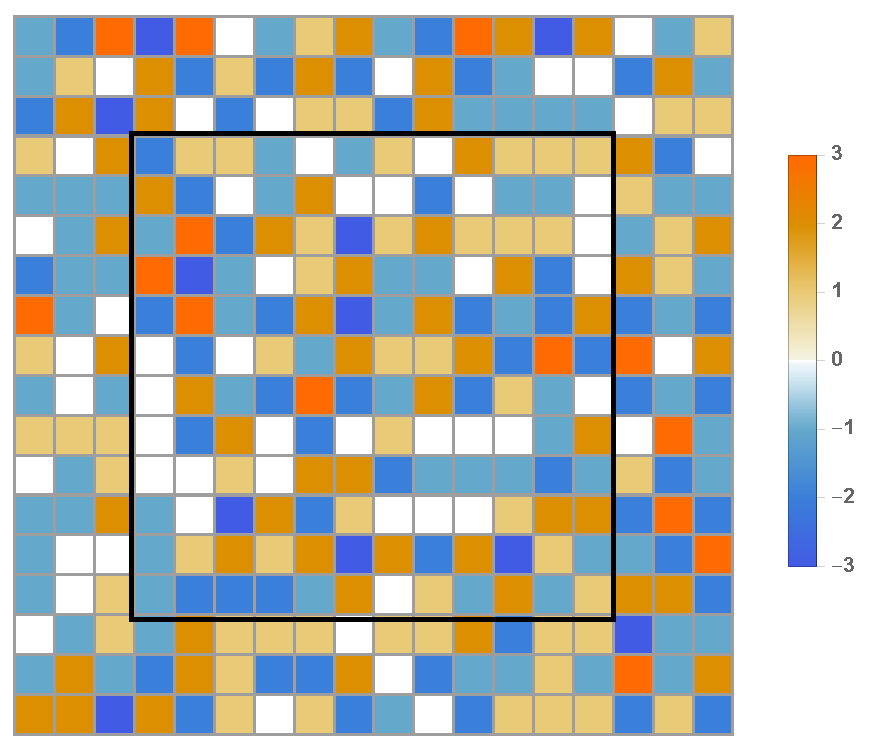
\includegraphics[width=0.40\textwidth]{HL18Shadowing12SourceA}
(b)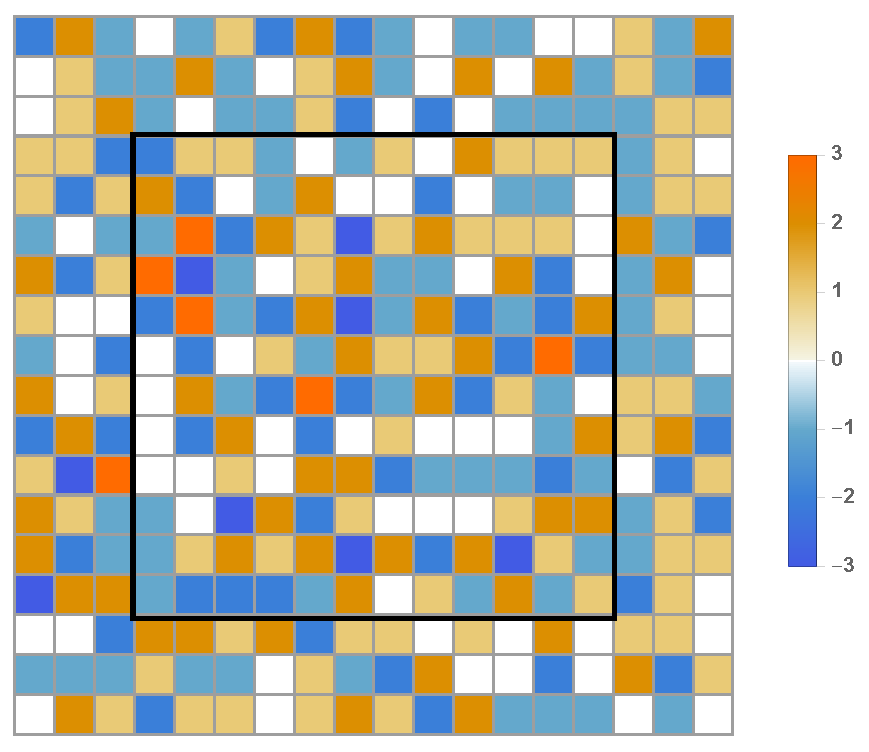
\includegraphics[width=0.40\textwidth]{HL18Shadowing12SourceB}
  \caption{\label{fig:HL18Shadowing12Source}
(a) and (b) are two {\admissible} [18$\times$18] \brick s corresponding to the two
distinct \twots\ of \reffig{fig:HL18Shadowing12Field}. They coincide within the shared
[12$\times$12] \brick\  $\Mm_\R$, region $\R$ indicated by the black border.
}
\end{figure}
%%%%%%%%%%%%%%%%%%%%%%%%%%%%%%%%%%%%%%%%%%%%%%%%%%%%%%%%%%%%%%%

%%%%%%%%%%%%%%%%%%%%%%%%%%%%%%%%%%%%%%%%%%%%%%%%%%%%%%%%%%%%%
\begin{figure}
  \centering
(a)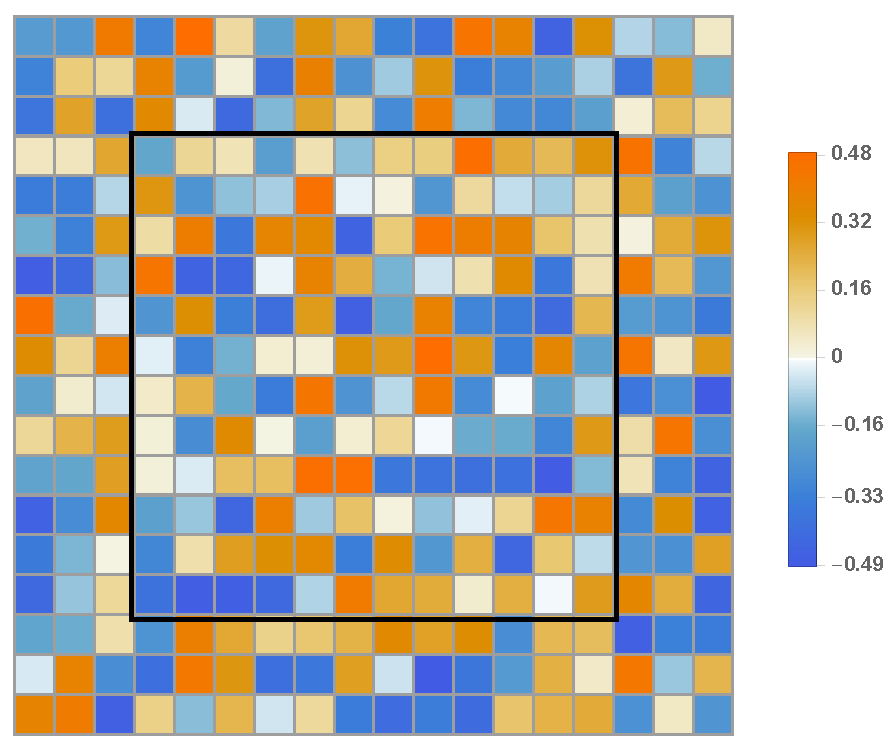
\includegraphics[width=0.40\textwidth]{HL18Shadowing12FieldA}
(b)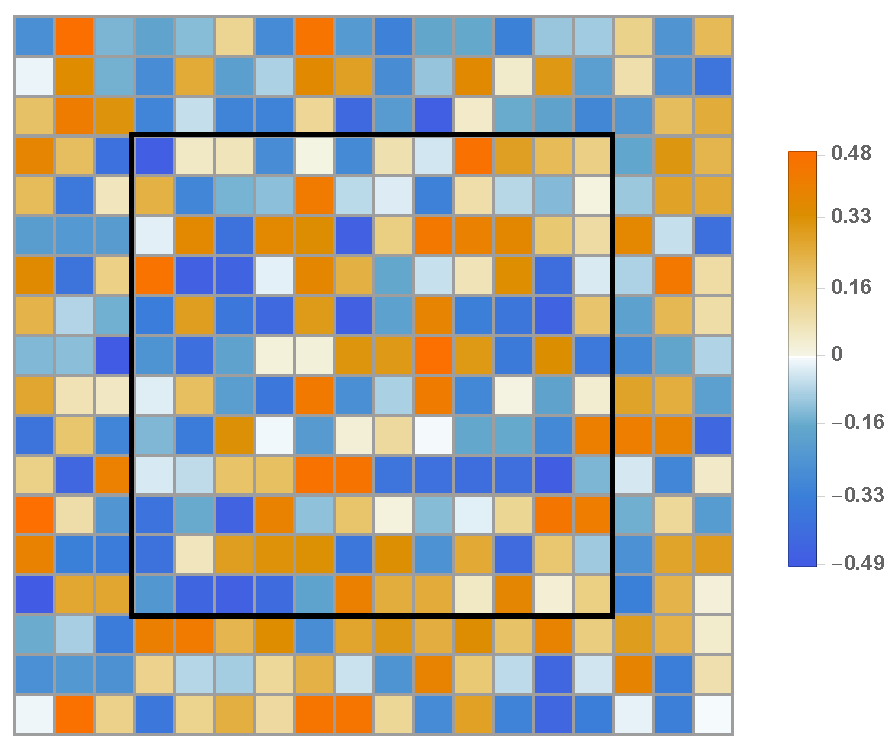
\includegraphics[width=0.40\textwidth]{HL18Shadowing12FieldB}
  \caption{\label{fig:HL18Shadowing12Field}
(a) and (b) are two \twots\ whose symbol arrays are given by the $[18\times18]$ \brick s of symbols of \reffig{fig:HL18Shadowing12Source}.
}
\end{figure}
%%%%%%%%%%%%%%%%%%%%%%%%%%%%%%%%%%%%%%%%%%%%%%%%%%%%%%%%%%%%%%%

%%%%%%%%%%%%%%%%%%%%%%%%%%%%%%%%%%%%%%%%%%%%%%%%%%%%%%%%%%%%%
\begin{figure}
  \centering
(a)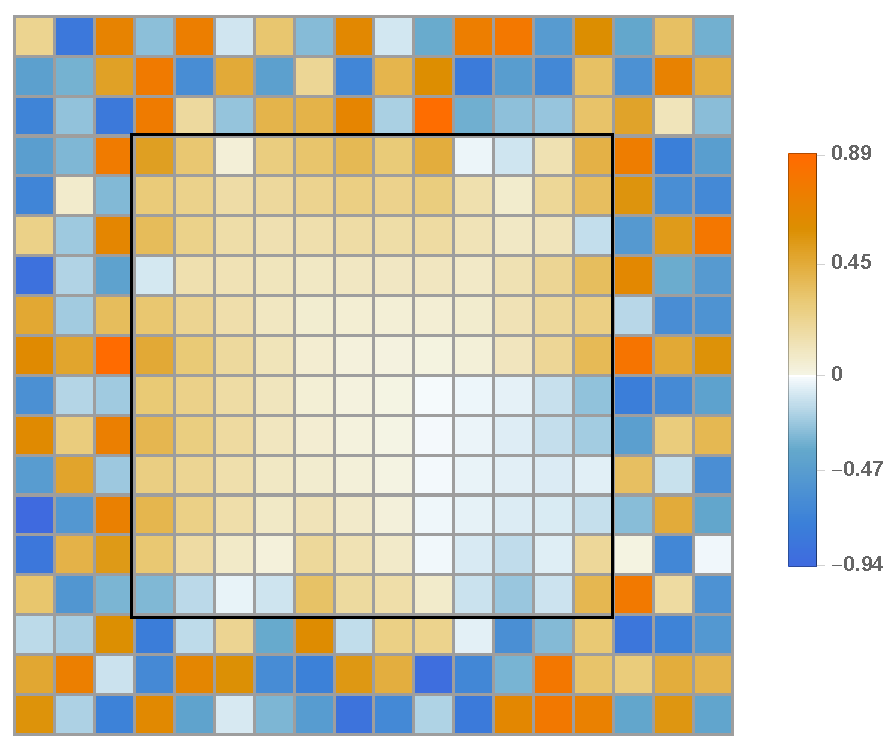
\includegraphics[width=0.40\textwidth]{HL18Shadowing12FieldDistance}
(b)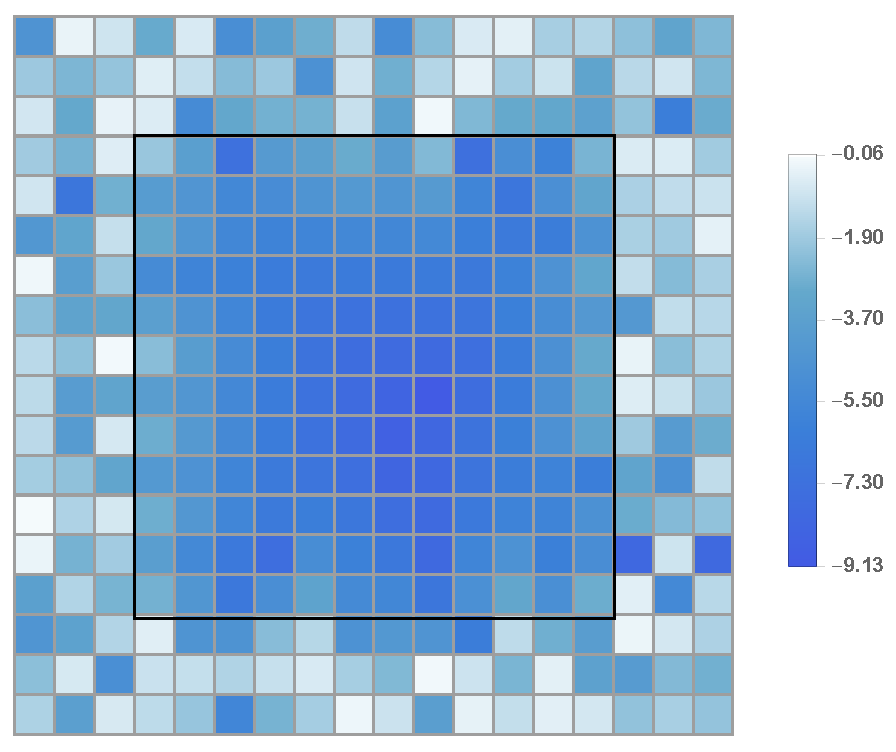
\includegraphics[width=0.40\textwidth]{HL18Shadowing12FieldDistanceLog}
  \caption{\label{fig:HL18Shadowing12Distance}
(a) The pointwise distance between the two \twots\ of \reffig{fig:HL18Shadowing12Field}.
(b) The logarithm of the absolute value of the distance between the two \twots\ indicate exponential shadowing close to the center of the shared $\Mm_\R$.
}
\end{figure}
%%%%%%%%%%%%%%%%%%%%%%%%%%%%%%%%%%%%%%%%%%%%%%%%%%%%%%%%%%%%%%%

	\HLpost{2019-08-21}{
I also did the shadowing plot of $[18\times18]$ \brick s with a smaller shared region of symbols. As shown in \reffigs{fig:HL18Shadowing8Source}{fig:HL18Shadowing8Field}, the shared region is a $[8\times8]$ \brick.

What I'm considering is: the symbols are on \twots,  so as we go further from the center of the shared region, we are getting closer to the shared region of the next tile. Using a smaller shared region we can probably reduce the effect of the next shared region. But compare \reffig{fig:HL18Shadowing12Distance} (b) and \reffig{fig:HL18Shadowing8Distance} (b), the logarithm of the distance is not too different. So I guess we don't need these figures with small shared region...

Also I think this exponential shadowing only exist in the region with shared symbols? In \reffig{fig:HL18Shadowing12Distance} (b) and \reffig{fig:HL18Shadowing8Distance} (b), the distance outside of the shared region looks random, while the distance within the shared region shrink exponentially as we go closer to the center.
	}
	
%%%%%%%%%%%%%%%%%%%%%%%%%%%%%%%%%%%%%%%%%%%%%%%%%%%%%%%%%%%%%
\begin{figure}
  \centering
(a)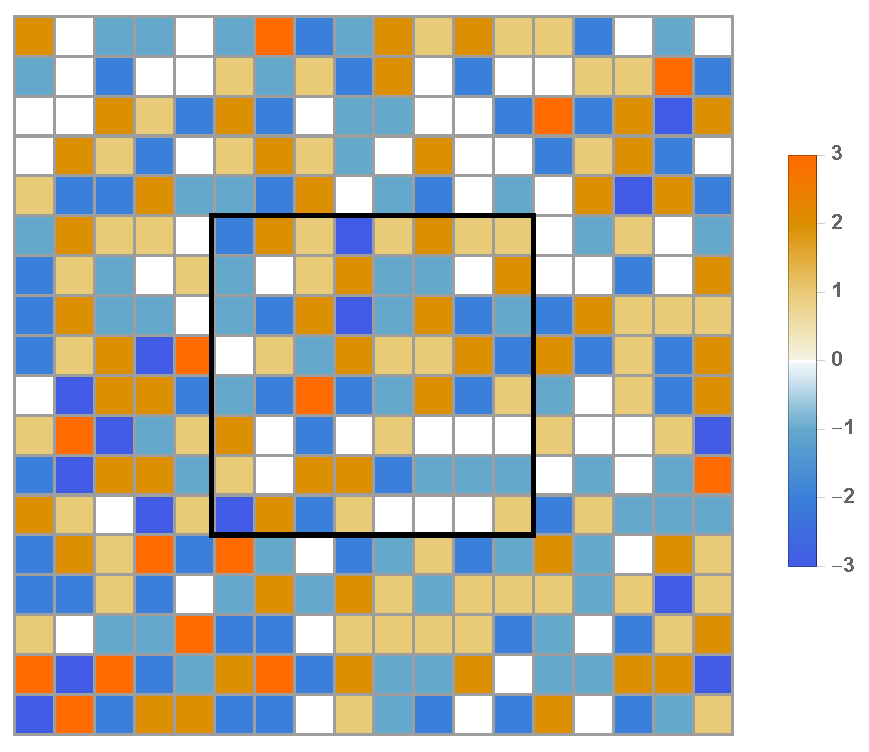
\includegraphics[width=0.40\textwidth]{HL18Shadowing8SourceA}
(b)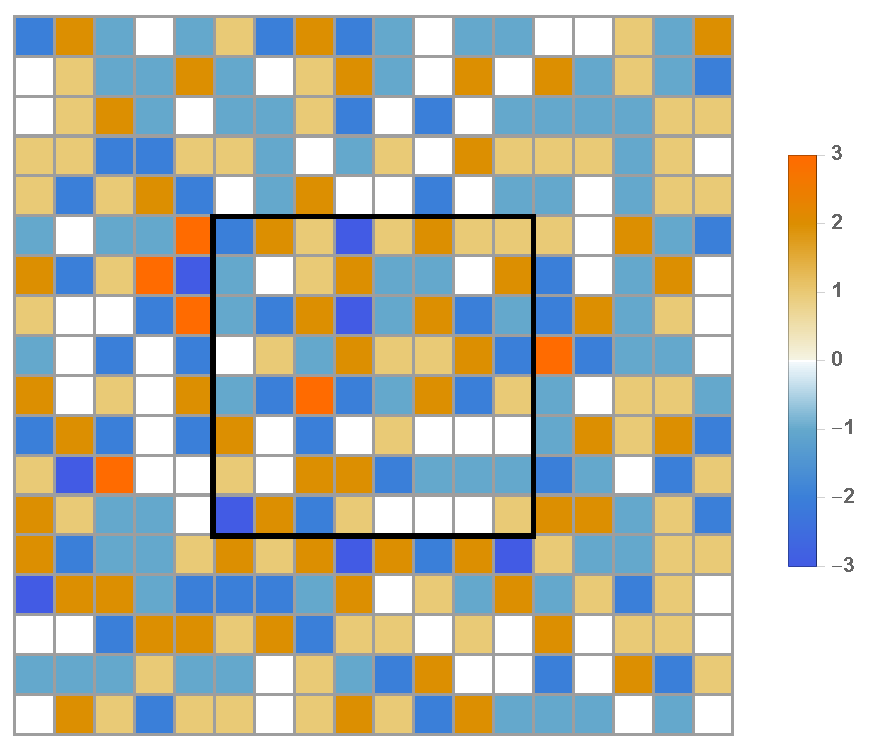
\includegraphics[width=0.40\textwidth]{HL18Shadowing8SourceB}
  \caption{\label{fig:HL18Shadowing8Source}
(a) and (b) are two {\admissible} [18$\times$18] \brick s corresponding to the two
distinct \twots\ of \reffig{fig:HL18Shadowing8Field}. They coincide within the shared
[8$\times$8] \brick\  $\Mm_\R$, region $\R$ indicated by the black border.
}
\end{figure}
%%%%%%%%%%%%%%%%%%%%%%%%%%%%%%%%%%%%%%%%%%%%%%%%%%%%%%%%%%%%%%%

%%%%%%%%%%%%%%%%%%%%%%%%%%%%%%%%%%%%%%%%%%%%%%%%%%%%%%%%%%%%%
\begin{figure}
  \centering
(a)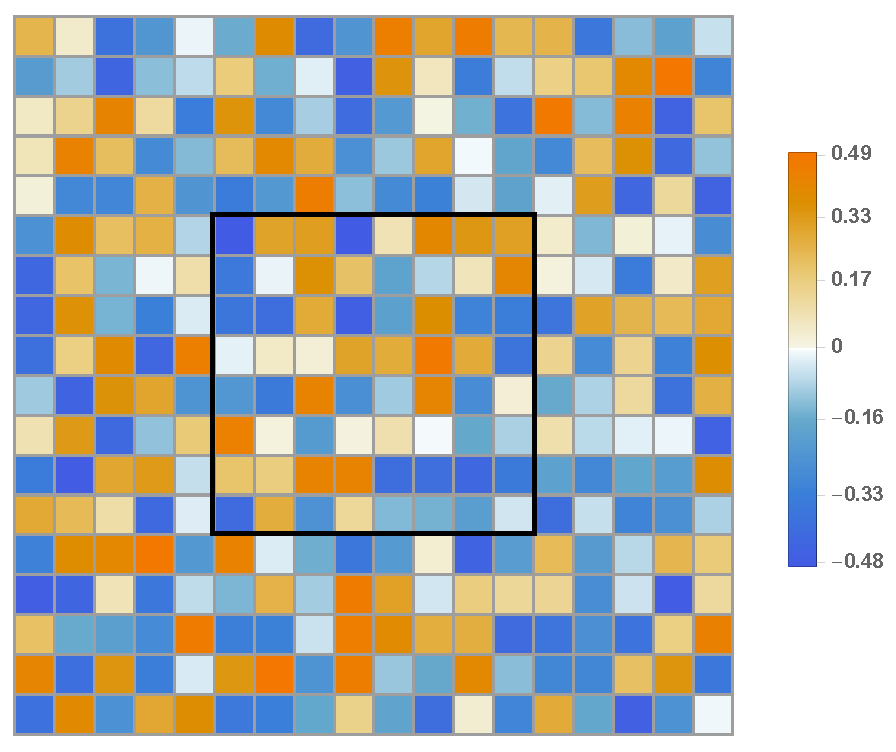
\includegraphics[width=0.40\textwidth]{HL18Shadowing8FieldA}
(b)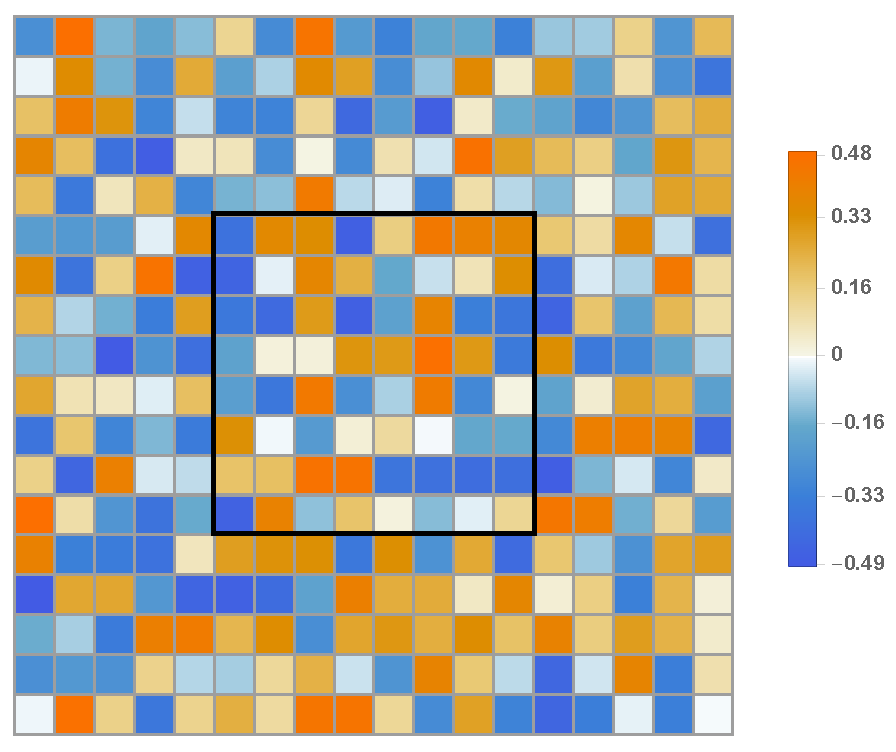
\includegraphics[width=0.40\textwidth]{HL18Shadowing8FieldB}
  \caption{\label{fig:HL18Shadowing8Field}
(a) and (b) are two \twots\ whose symbol arrays are given by the $[18\times18]$ \brick s of symbols of \reffig{fig:HL18Shadowing8Source}.
}
\end{figure}
%%%%%%%%%%%%%%%%%%%%%%%%%%%%%%%%%%%%%%%%%%%%%%%%%%%%%%%%%%%%%%%

%%%%%%%%%%%%%%%%%%%%%%%%%%%%%%%%%%%%%%%%%%%%%%%%%%%%%%%%%%%%%
\begin{figure}
  \centering
(a)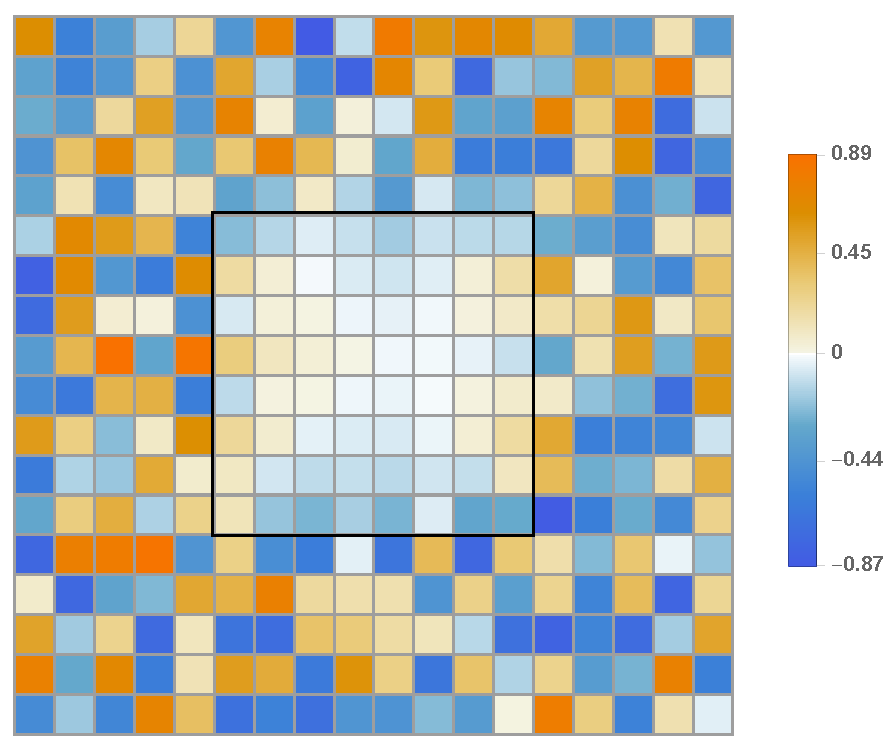
\includegraphics[width=0.40\textwidth]{HL18Shadowing8FieldDistance}
(b)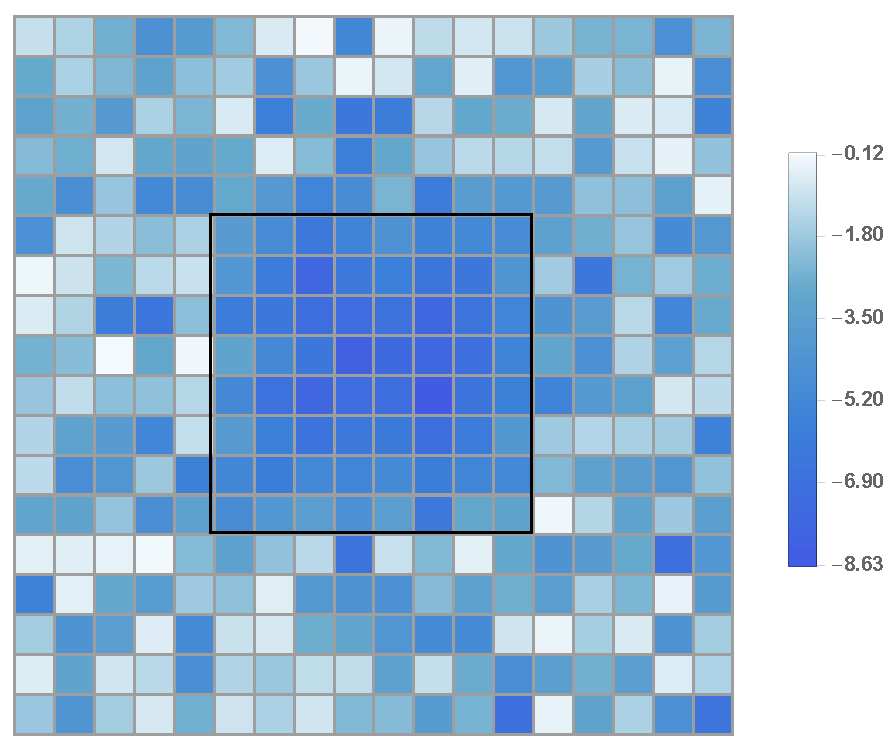
\includegraphics[width=0.40\textwidth]{HL18Shadowing8FieldDistanceLog}
  \caption{\label{fig:HL18Shadowing8Distance}
(a) The pointwise distance between the two \twots\ of \reffig{fig:HL18Shadowing8Field}.
(b) The logarithm of the absolute value of the distance between the two \twots\ indicate exponential shadowing close to the center of the shared $\Mm_\R$.
}
\end{figure}
%%%%%%%%%%%%%%%%%%%%%%%%%%%%%%%%%%%%%%%%%%%%%%%%%%%%%%%%%%%%%%%

	\HLpost{2019-08-21}{
Another thing I tried is to generate 11 different $[18\times18]$ \twots\ shared a same $[12\times12]$ \brick\ of symbols. Take one of these \twots\ and compute the distance between this \twot\ and other 10 \twots, then compute the ensemble average. The result is shown in \reffig{fig:HL18Shadowing12DistanceAverage}, which looks very similar to \reffig{fig:HL18Shadowing12Distance}. Perhaps using a larger group of ensemble we can get a better result?
	}
	
%%%%%%%%%%%%%%%%%%%%%%%%%%%%%%%%%%%%%%%%%%%%%%%%%%%%%%%%%%%%%
\begin{figure}
  \centering
(a)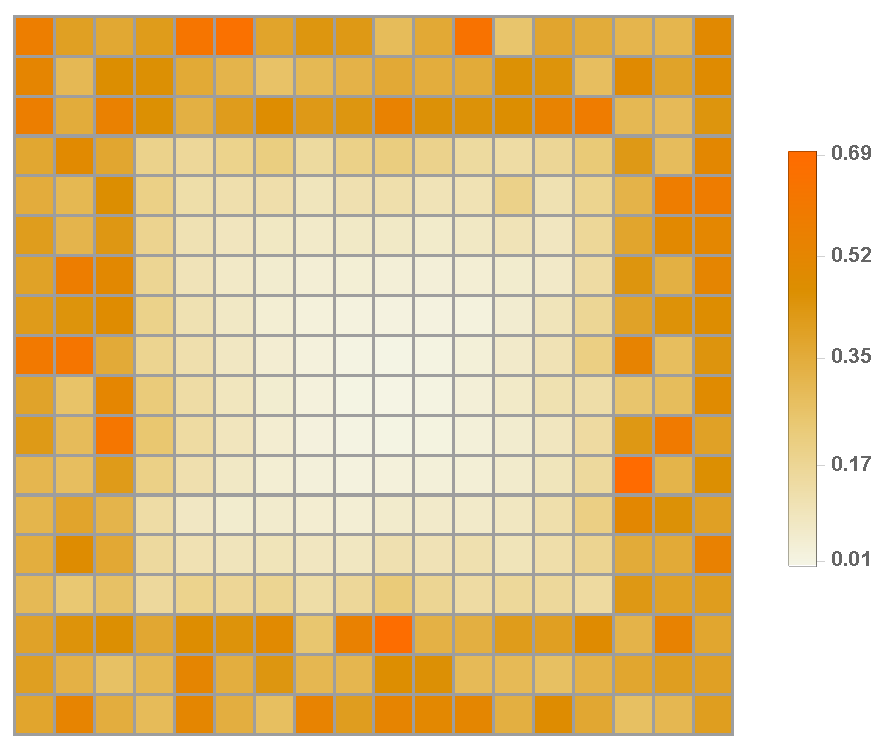
\includegraphics[width=0.40\textwidth]{HL18ShadowingDistanceAverage}
(b)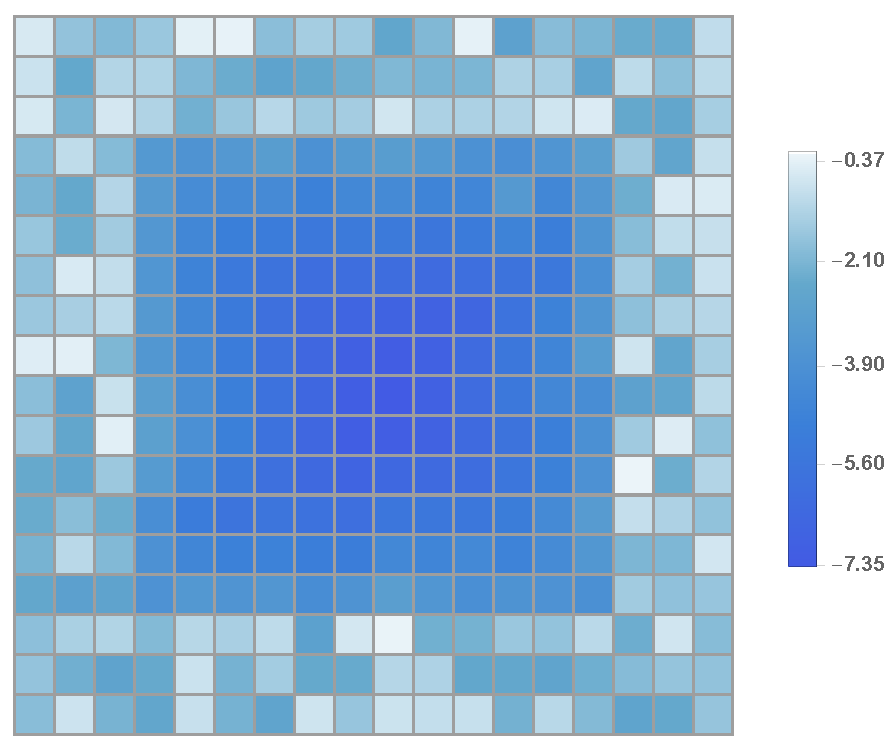
\includegraphics[width=0.40\textwidth]{HL18ShadowingDistanceAverageLog}
  \caption{\label{fig:HL18Shadowing12DistanceAverage}
(a) The average of the absolute value of the pointwise distance between the one \twot\ and other 10 different \twots\ with shared $[12\times12]$ \brick\ of symbols.
(b) The logarithm of the average of the absolute value of the distance between the \twots\ indicate exponential shadowing close to the center of the shared $\Mm_\R$.
}
\end{figure}
%%%%%%%%%%%%%%%%%%%%%%%%%%%%%%%%%%%%%%%%%%%%%%%%%%%%%%%%%%%%%%%

	\HLpost{2019-08-22}{
I generated 500 different \twots\ with a shared $[12\times12]$ \brick\ of symbols at the center, labeled as $\Xx_1, \Xx_2, \dots, \Xx_{500}$. Then I compute the distance between $\Xx_i$ and $\Xx_{i+250}$ where $i$ goes from 1 to 250, and get 250 distance field. \refFig{fig:HL18ShadowingDistanceAverage3D} is the log plot of the absolute value of the distance field. \refFig{fig:HL18ShadowingDistanceAverage3D} (a) is the logarithm of the distance between field $\Xx_1$ and $\Xx_{251}$, and (b) is the the logarithm of the average of the 250 distance field. By doing the average, the distance field becomes smooth. \refFig{fig:HL18ShadowingDistanceAverageCrossSection} is the cross section of \reffig{fig:HL18ShadowingDistanceAverage3D} through the center of the field. In \reffig{fig:HL18ShadowingDistanceAverageCrossSection} (b) the logarithm of the distance is straight line in the region with shared symbols, which shows that the distance shrink exponentially as getting closer to the center.

In \reffig{fig:HL18ShadowingDistanceAverageCrossSection} (b), the logarithm of the distance outside of the shared symbol \brick\ is approximately equal to $\ln(1/3) = -1.0986$, where $1/3$ is the average distance between two random numbers within the range $[-1/2, 1/2)$.

I still need to add axis labels to these figures... (It seems like Mathematica doesn't allow me to use LaTeX for writing the labels.)
	}

%%%%%%%%%%%%%%%%%%%%%%%%%%%%%%%%%%%%%%%%%%%%%%%%%%%%%%%%%%%%%
\begin{figure}
  \centering
(a)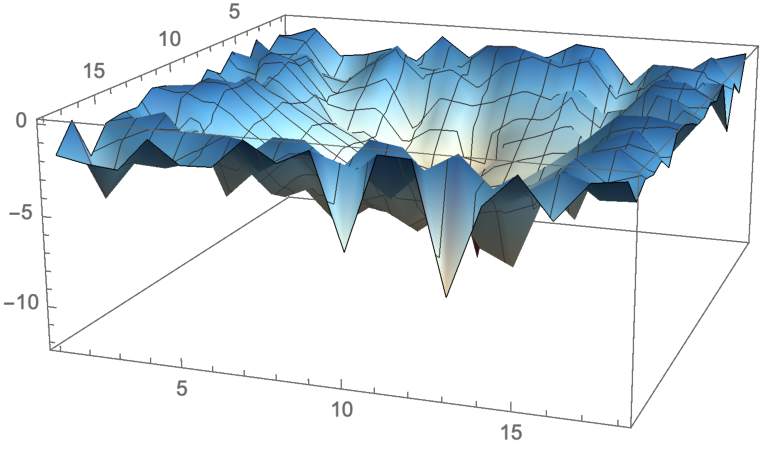
\includegraphics[width=0.40\textwidth]{HL18ShadowingDistanceLog3D}
(b)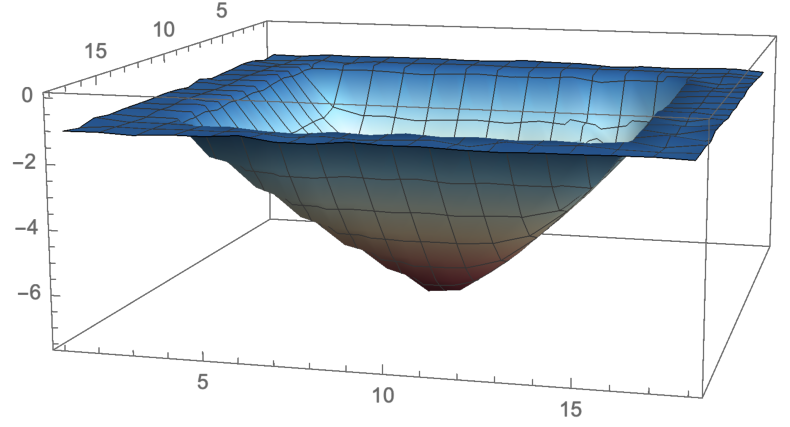
\includegraphics[width=0.40\textwidth]{HL18ShadowingDistanceAverageLog3D}
  \caption{\label{fig:HL18ShadowingDistanceAverage3D}
(a) The logarithm of the absolute value of the pointwise distance between the solutions $\Xx_1$ and $\Xx_{251}$ with shared $[12\times12]$ \brick\ of symbols at the center.
(b) The logarithm of the average of the absolute value of 250 different distance fields.
}
\end{figure}
%%%%%%%%%%%%%%%%%%%%%%%%%%%%%%%%%%%%%%%%%%%%%%%%%%%%%%%%%%%%%%%

%%%%%%%%%%%%%%%%%%%%%%%%%%%%%%%%%%%%%%%%%%%%%%%%%%%%%%%%%%%%%
\begin{figure}
  \centering
(a)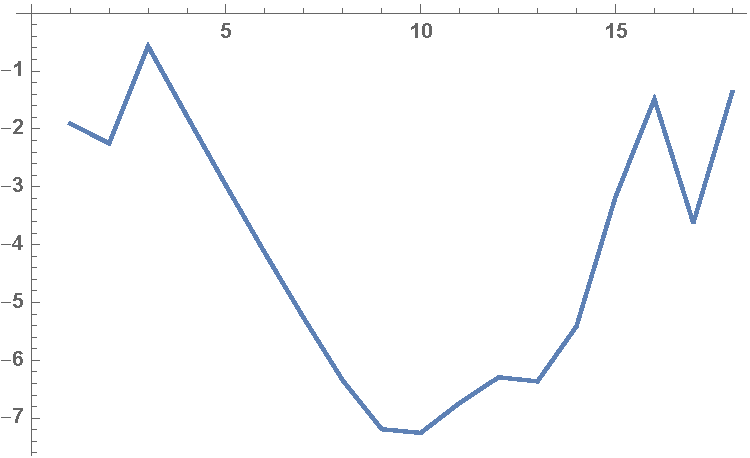
\includegraphics[width=0.40\textwidth]{HL18ShadowingDistanceLogCrossSection}
(b)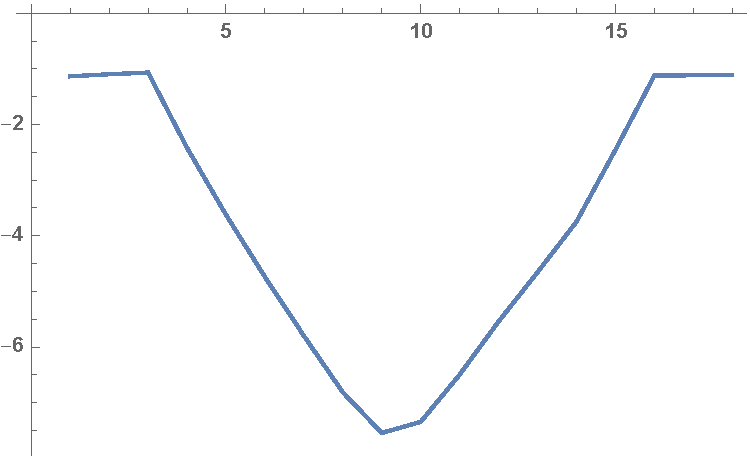
\includegraphics[width=0.40\textwidth]{HL18ShadowingDistanceAverageLogCrossSection}
  \caption{\label{fig:HL18ShadowingDistanceAverageCrossSection}
(a) The cross section through the center of the \reffig{fig:HL18ShadowingDistanceAverage3D} (a).
(b) The cross section through the center of the \reffig{fig:HL18ShadowingDistanceAverage3D} (b). The logarithm of the distance decreases linearly as the coordinate of the field approaches the center of the shared symbol \brick.
}
\end{figure}
%%%%%%%%%%%%%%%%%%%%%%%%%%%%%%%%%%%%%%%%%%%%%%%%%%%%%%%%%%%%%%%


	\PCpost{2019-09-05}{dropped this:\\
\( %\beq
(\ssp \mapsto A \ssp
    \,%\qquad
|\,
\ssp
    % = \left(\begin{array}{c} \coord\\p \end{array} \right )
  \in \mathbb{T}^2 =  \reals^2/\integers^2
    \,;\; %\qquad
A \in \SLn{2}{\integers}
)
\,,
\) %\ee{LinSympMap}

on no time-forward map,

\bigskip
In \refappe{s:GenFctn} we derive the Lagrangian formulation of cat maps.

Cat map is so simple that going from Hamiltonian to Lagrangian
formulation amounts to replacement \refeq{Ham2Lagr} of momentum
by velocity.
Still, for what follows, it might pay off to understand the general
theory of transformations from discrete Hamiltonians to discrete
Lagrangians; we review that in  refappe {s:GenFctn}.

The new results follow from our determination of \statesp\ generating partitions
generated by the iterations of the cat map, for different integer values
of the stretching parameter $s$.

, new kinds of
determinants, new relations between propagation of temporal vs. spatial
disturbances; some of these are derived in XXX eq.~{s:Green}.

Following eqs. {PerViv2.1a} and {PerViv2.1b}:
Here $2\pi \coord$ is the  angle of the rotor, $p$ is the
momentum conjugate to the angular coordinate $\coord$, the angular pulse
$P(\coord)=P(\coord+1)$ is periodic with period $1$, and the time step
has been set to $\Delta\zeit= 1$.
Eq.~\refeq{PerViv2.1b} says that in one time step $\Delta\zeit$ the
configuration trajectory starting at $\coord_{\zeit}$ reaches
$\coord_{\zeit+1} = \coord_{\zeit}+p_{\zeit+1}\Delta {\zeit}$,
and
\refeq{PerViv2.1a} says that at each kick the angular momentum
$p_{\zeit}$ is accelerated to $p_{\zeit+1}$ by the force
$P(\coord_{\zeit})\Delta\zeit$.
As the values of $\coord$ differing by integers are identified, and the
momentum $p$ is unbounded, the phase space is a cylinder. However, one
can analyze the dynamics just as well on the compactified phase space,
with the momentum wrapped around a circle, \ie, adding $\mod 1$ to
\refeq{PerViv2.1a}. Now the dynamics is a toral automorphism acting on a
$(0,1]\times(0,1]$ phase space square of unit area, with the opposite
edges identified.

We shall refer here to the least unstable of the cat maps
\refeq{catMap}, with $s=3$, as the `Arnol'd cat
map'\rf{ArnAve,deva87}, and to maps with integer $s\geq 3$ as `cat
maps'.

For {\catlatt} \refeq{CatMap2d} the field $\ssp_{n\zeit}$ takes values in
the $\speriod{}\period{}$\dmn\ unit hyper-cube
$\Xx\in[0,1)^{\speriod{}\period{}}$, where $\speriod{}$ is the `spatial',
and $\period{}$ the `temporal' lattice period.

    }

	\PCpost{2019-12-15}{move to GuBuCv17.tex:\\
Flows described by {\pdes} are in principle infinite dim\-ens\-ion\-al,
and, at first glance, turbulent dynamics that they exhibit might appear
hopelessly complex. However, what is actually observed in experiments and
simulations is that turbulence is dominated by repertoires of
identifiable recurrent vortices, rolls, streaks and the
like\rf{science04}. Dynamics on a low-dim\-ens\-ion\-al chaotic attractor
can be visualized as a succession of near visitations to exact unstable
periodic  solutions of the equations of motion, interspersed by transient
interludes\rf{DasBuch}. In the same spirit, the long-term turbulent
dynamics  of spatially   extended systems can  be thought of as a
sequence of visitations through the repertoire of {\admissible}  {\spt}
patterns, each framed by a finite {\spt}
window. The question we address here is: can states of a strongly
nonlinear field theory  be described by such repertoires of {\admissible}
patterns explored by turbulence?
And if yes, what is the likelihood to observe any such pattern?

Such  questions have been   studied  extensively for systems of  small
spatial extension, where the attractor dimension is relatively
small\rf{Christiansen97,SCD07,CviGib10,ACHKW11,KreEck12}.
However, going from  spatially small to spatially infinite systems
will require completely new tools.
For small systems the
long time dynamics can be thought of as motion of a point within an
inertial  manifold  of a moderate dimension.

    }



	\PCpost{2019-12-14}{restore this somewhere in cat map discussions:\\
The key property of hyperbolic flows is that nearby trajectories can
\emph{shadow} each other for finite times controlled by their stability
exponents. One common way to quantify `nearness' is to determine the
minimal Euclidean distance between pairs of trajectories. That kind of
distance is not invariant under symplectic transformations, and is thus
meaningless in the Hamiltonian phase space. Here the notion of action
comes to rescue:
\emph{the symplectic invariant distance between a pair of shadowing
orbits is given by the difference of their actions}\rf{LiTom17b}.
    }

    \PCpost{2019-12-20}{dropped\\
Incorporate \emph{spatiotemp/Examples/tempStab3cyc.tex},
eq.~{tempStab3cyc:inv}
    }

    \PCpost{2020-01-13}{Implemented now in the article:\\
I know LU is a method in textbooks, but in this example, cannot you use
the periodicity of $\shift$, as I do in \refsect{s:bernCount}~{\em
Counting Bernoulli \po s}, \refsect{exam:tempStab3cyc}~{\em Temporal
lattice stability of a 3-cycle}, but for $d$\dmn\ example done here?
\refeq{dDmnForwardJacobianB} is the same as \refeq{LnDet=TrLn}, but for a
$d$\dmn\ \jacobianM\ $\jMat$, rather than the $1$\dmn\ matrix ${s}$.
    }

    \PCpost{2019-08-04}{
to Han - Please make sure that all definitions and signs
agree with the discrete lattice sections of ChaosBook\rf{DasBuch}.
                    }

\HLpost{2020-01-28}{
To prove that the product of cosines gives Chebyshev polynomial, the
simplest way is to use the identity from Grashteyn and Ryzhik\rf{GraRyz}
{\em Table of Integrals, Summations and Products}
(Academic Press, New York, 1965) 1.395.2:
\beq
\cosh nx -\cos ny
  = 2^{n-1} \prod_{k=0}^{n-1} \big\{ \cosh x - \cos(y+\frac{2 k \pi}{n}) \big\}
\, .
\label{TableOfISP13952}
\eeq
Let $y=0$, $\cosh x = s/2$, and multiply both side by 2, \refeq{TableOfISP13952} becomes:
\beq
\prod_{k=0}^{n-1} \big\{ s - 2 \cos(\frac{2 k \pi}{n}) \big\}
=2 \{\cosh[n \, \mbox{arcosh}(s/2)] - 1\}
\, .
\label{TableOfISP13952-2}
\eeq
By the definition of the Chebyshev polynomials of the first kind:
\[
T_n(x) = \cosh(n \, \mbox{arcosh} \, x), \quad \mbox{if} \, x \geq 1 \, ,
\]
the right hand side of \refeq{TableOfISP13952-2} is $2\,T_{n}(s/2) -2$,
same as \refeq{POsChebyshev}.

%Using the standard theory of Toeplitz matrices (or the orthonormality of
%discrete Fourier eigenmodes, see \refappe{appe:Fourier}), one can write
%determinant \refeq{POsChebyshev} compactly as
%\beq
%N_\cl{} = \det \jMorb
% = 2\,T_{\cl{}}(s/2) -2
%% = \ExpaEig^{\cl{}} + \ExpaEig^{-\cl{}} - 2
%\,,
%\label{POsChebyshevFT}
%\eeq
%where $T_{\cl{}}(s/2)$ is the Chebyshev polynomial of the first kind.
%
%Or, without any explicit reference to Chebyshev polynomials, see
%\refeq{Isola90-13} below.
     } %\HLpost{2020-01-28}{

    \PCpost{2019-12-18}{
turn the final version into
\emph{spatiotemp/chapter/examSawtoothLin.tex} examples,
then move to ChaosBook.
    }


%    \PCpost{2019-12-24}{
%Thanks for catching my sign error.
%Is the derivation of \refeq{detBern2}
%OK now?
%    }

    \HLpost{2020-01-17}{
For
a {\lattstate} $\Xx_\Mm$ with period $\cl{}$, the \jacobianOrb\
\refeq{jacobianOrb} is a $[\cl{}d\times\cl{}d]$ block matrix
\beq
\begin{array}{cc}
 \\ \\ \jMorb & = \\ \\
\end{array}
\left(
\begin{array}{ccccc}
\id & & & & -\jMat \\
-\jMat & \id & \\
& ~~\cdots~~ & \id \\
 & & ~~\cdots~~ & \id \\
 & & &-\jMat & \id
\end{array}
\right)
= \id-\jMat \otimes \shift^{-1}
\,,
\ee{dDmnForwardJacobianB}
where $\id$ is a $d$\dmn\ identity matrix, $\jMat$ is the one time
step $[d\times d]$ \jacobianM\ \refeq{dDmn1stepJac1}, and $\shift$ is
the $[\cl{} \times \cl{}]$ {\shiftOp} matrix with period $\cl{}$.

To evaluate the determinant of the \jacobianOrb, expand $\ln \det \jMorb = \tr \ln \jMorb$:
\bea
\ln \det \jMorb
&=& \tr \ln (\id-\jMat \otimes \shift^{-1}) \continue
&=& - \sum_{k=1}^{\infty} \frac{1}{k}\tr (\jMat \otimes \shift^{-1})^k
\, .
\label{dDmnForwardJacobianLnDet}
\eea
Note that $(\jMat \otimes \shift^{-1})^k = \jMat^k \otimes \shift^{-k}$ and
$\tr (\jMat^k \otimes \shift^{-k})
= \tr (\jMat^{\cl{}r} \otimes \id_{[\cl{}\times\cl{}]}) \delta_{k,\cl{}r}
= \cl{} \tr (\jMat^{\cl{}r}) \delta_{k,\cl{}r}
$
 which is not 0 only when $k$ is a multiple of $\cl{}$.
\bea
\ln \det \jMorb
&=& - \sum_{r=1}^{\infty} \frac{\cl{} \tr (\jMat^{r\cl{}})}{r\cl{}}
 =  \tr [- \sum_{r=1}^{\infty} \frac{(\jMat^{\cl{}})^r}{r}] \continue
&=& \tr \ln (\id - \jMat^{\cl{}})
 =  \ln \det (\id - \jMat^{\cl{}})
\, .
\label{dDmnForwardJacobianLnDet2}
\eea
So the determinant of the \jacobianOrb\ is $\det \jMorb = \det (\id - \jMat^{\cl{}})$.


hence
\beq
\det \jMorb_\Mm
=
    \det(\jMat_\Mm-\id)
=
    \det(\jMat^\cl{} - \id)
\,.
\label{bernNotHill}
\eeq
}

\HLpost{2020-01-21}{
A possible problem is $\jMorb$ could be negative. And here we have the one time step
 \jacobianM\ instead of a scalar $s$ so I'm not sure if we can expand $\ln (\id-\jMat \otimes \shift^{-1})$
 as a series in $\jMat \otimes \shift^{-1}$...
}

\HLpost{2020-01-13}{
\refeq{NotHillDeterminant} is different from \refeq{bernNotHill}. I think
\refeq{NotHillDeterminant} is correct. Will check again.
}

    \PCpost{2020-01-13}{
You are right about the sign - I was hoping to avoid $N_\cl{} =
|\det \jMorb|$ in \refeq{detBern0}, but I cannot change the sign of the
matrix $\jMorb$ without making the fixed {point} condition
\refeq{tempBern} look awkward.
    }

    \PCpost{2020-01-24}{
I think (now commented out) \reffig{fig:FundPar}\,(b) was illegal - we
are not allowed to define a Bravais cell off the unit cell, on the 1/2
integer lattice. Removed, unless Han has a counterargument. It is kept
for the record in \emph{spatiotemp/chapter/catHamilton.tex}
    }

\HLpost{2020-01-21}{
A possible problem with \refeq{detDet} is that $\jMorb$ could be
negative. And here we have the one time step \jacobianM\ instead of a
scalar $s$ so I'm not sure if we can expand $\ln (\id-\jMat \otimes
\shift^{-1})$ as a series in $\jMat \otimes \shift^{-1}$...
}

    \PCpost{2020-01-27}{Dropped:
This overcounting happens if the initial unit square is on the integer
lattice. If initial states lie off the integer lattice, within the
symmetric unit square $(-1/2,1/2]\times(-1/2,1/2]$ (Wigner-Seitz cell?),
the fundamental parallelogram \reffig{fig:FundPar}\,(b) all 5 integer
points lie within the fundamental parallelogram, without any
over-counting. This is not the situation studied here, so we will not
pursue it further.

We are not aware of any useful visualizations of {\jacobianOrb}
{\fundPip} for $n > 3$ \templatt\ and 2- and $d$\dmn\
\catlatt\ of \refsect{s:catlatt}.

---------------------------------------------------------------
\[
(- \Box +s -4)_{0,0,i_2, j_2} = (\jMorb_{0,0})_{i_2, j_2} =
 \left[
 \begin{array}{ccc}
 -1 & -1 & 0 \\
 5 & -1 & -1
 \end{array}
 \right]_{i_2, j_2} \, ,
\]
\[
 (- \Box +s -4)_{0,1,i_2, j_2} = (\jMorb_{0,1})_{i_2, j_2} =
 \left[
 \begin{array}{ccc}
 5 & -1 & -1 \\
 -1 & 0 & -1
 \end{array}
 \right]_{i_2, j_2} \, ,
\]
\[
 (- \Box +s -4)_{1,0,i_2, j_2} = (\jMorb_{1,0})_{i_2, j_2} =
 \left[
 \begin{array}{ccc}
 0 & -1 & -1 \\
 -1 & 5 & -1
 \end{array}
 \right]_{i_2, j_2} \, ,
\]
\[
 (- \Box +s -4)_{1,1,i_2, j_2} = (\jMorb_{1,1})_{i_2, j_2} =
 \left[
 \begin{array}{ccc}
 -1 & 5 & -1 \\
 -1 & -1 & 0
 \end{array}
 \right]_{i_2, j_2} \, ,
\]
\[
 (- \Box +s -4)_{2,0,i_2, j_2} = (\jMorb_{2,0})_{i_2, j_2} =
 \left[
 \begin{array}{ccc}
 -1 & 0 & -1 \\
 -1 & -1 & 5
 \end{array}
 \right]_{i_2, j_2} \, ,
\]
\[
 (- \Box +s -4)_{2,1,i_2, j_2} = (\jMorb_{2,1})_{i_2, j_2} =
 \left[
 \begin{array}{ccc}
 -1 & -1 & 5 \\
 0 & -1 & -1
 \end{array}
 \right]_{i_2, j_2} \, .
\]
To diagonalize this rank-4 {\jacobianOrb} we need to use the the eigenvectors \refeq{2DEigenvector} to form a rank-4 tensor:
\[
U_{i_1,j_1,i_2,j_2}=
\exp\left(
      i\frac{2 \pi}{6}(2 i_2 i_1 - i_2 j_1 + 3 j_2 j_1)
        \right) \, .
\]
The inverse of this tensor is the conjugate transpose $U^\dagger$:
\[
(U^\dagger)_{i_1,j_1,i_2,j_2} = (U_{i_2,j_2,i_1,j_1})^* \, .
\]
The diagonalized {\jacobianOrb} is:
\[
(\jMorb_{\mathrm{diagonalized}})_{i_1,j_1,i_2,j_2}
= \sum_{i_3=0}^2 \sum_{j_3=0}^1 \sum_{i_4=0}^2 \sum_{j_4=0}^1 (U^\dagger)_{i_1,j_1,i_3,j_3} \jMorb_{i_3,j_3,i_4,j_4} U_{i_4,j_4,i_2,j_2} \, .
\]
The diagonalized {\jacobianOrb}'s element $(\jMorb_{\mathrm{diagonalized}})_{i_1,j_1,i_2,j_2}$ is not 0 only when $i_1 = i_2$ and $j_1 = j_2$. We can get the inverse of this diagonalized tensor, $\jMorb_{\mathrm{diagonalized}}^{-1}$, by changing the non-zero elements to their inverse. Then inverse of the {\jacobianOrb} is:
\[
(\jMorb^{-1})_{i_1,j_1,i_2,j_2} =
\sum_{i_3=0}^2 \sum_{j_3=0}^1 \sum_{i_4=0}^2 \sum_{j_4=0}^1 U_{i_1,j_1,i_3,j_3} (\jMorb_{\mathrm{diagonalized}}^{-1})_{i_3,j_3,i_4,j_4} (U^\dagger)_{i_4,j_4,i_2,j_2} \, .
\]
The elements of the inverse {\jacobianOrb} are:
\[
(\jMorb^{-1}_{0,0})_{i_2, j_2} = \frac{1}{35}
 \left[
 \begin{array}{ccc}
 5 & 5 & 4 \\
 11 & 5 & 5
 \end{array}
 \right]_{i_2, j_2} \, ,
\]
\[
(\jMorb^{-1}_{0,1})_{i_2, j_2} = \frac{1}{35}
 \left[
 \begin{array}{ccc}
 11 & 5 & 5 \\
 5 & 4 & 5
 \end{array}
 \right]_{i_2, j_2} \, ,
\]
\[
(\jMorb^{-1}_{1,0})_{i_2, j_2} = \frac{1}{35}
 \left[
 \begin{array}{ccc}
 4 & 5 & 5 \\
 5 & 11 & 5
 \end{array}
 \right]_{i_2, j_2} \, ,
\]
\[
(\jMorb^{-1}_{1,1})_{i_2, j_2} = \frac{1}{35}
 \left[
 \begin{array}{ccc}
 5 & 11 & 5 \\
 5 & 5 & 4
 \end{array}
 \right]_{i_2, j_2} \, ,
\]
\[
(\jMorb^{-1}_{2,0})_{i_2, j_2} = \frac{1}{35}
 \left[
 \begin{array}{ccc}
 5 & 4 & 5 \\
 5 & 5 & 11
 \end{array}
 \right]_{i_2, j_2} \, ,
\]
\[
(\jMorb^{-1}_{2,1})_{i_2, j_2} = \frac{1}{35}
 \left[
 \begin{array}{ccc}
 5 & 5 & 11 \\
 4 & 5 & 5
 \end{array}
 \right]_{i_2, j_2} \, .
\]
---------------------------------------------------------------

    }

    \PCpost{2020-01-30}{Dropped everything mentioning `Brillouin zones',
    for example   \reffig{fig:HLReciprocalLattice}\,(b);
they are OK for solid state physics, but our job is to count integer lattice
points, and Brillouin zones live off integer lattices.

Dropped: The periodicity of a periodic state  $\Xx({z})$ over a $d$\dmn\ lattice, with
the state described by repeats of a Bravais cell
spanned by basis vectors
\(({\bf a}_1,{\bf a}_2,\cdots,{\bf a}_d)\),
 \beq
\Lambda
= \left\{ \sum_{i=1}^d n_i {\bf a}_i\,\mid\,n_i \in \mathbb{Z}\right\}
\,.
\ee{dDBravaisLatt}

and combine them as columns of matrix
\beq
  \Lambda =
\left(\begin{array}{cc}
  \speriod{}&{S}\\
  0&\period{}
\end{array}\right)
\ee{Holmin12-Hermite2dOld}

\beq
\left[
\begin{array}{cc}
{\bf a}_1 & {\bf a}_2 \\
\end{array}
\right]
=
\left[
\begin{array}{cc}
 \speriod{} & {S} \\
 0 & \period{} \\
\end{array}
\right]
 \,.
\ee{2DBravaisBasis}

This is the simplest example
of a \catlatt\ tiling that is not just a 1\dmn\ {\templatt} \po\ solution
along one direction, repeated along the other.
    }


%%%%%%%%%%%%%%%%%%%%%%%%%%%%%%%%%%%%%%%%%%%%%%%%%%%%%%%%%%%%%
\begin{figure}
  \centering
% kept this(a)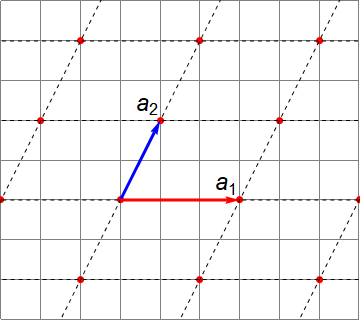
\includegraphics[width=0.40\textwidth]{HLBravaisLattice}
~~~
(b)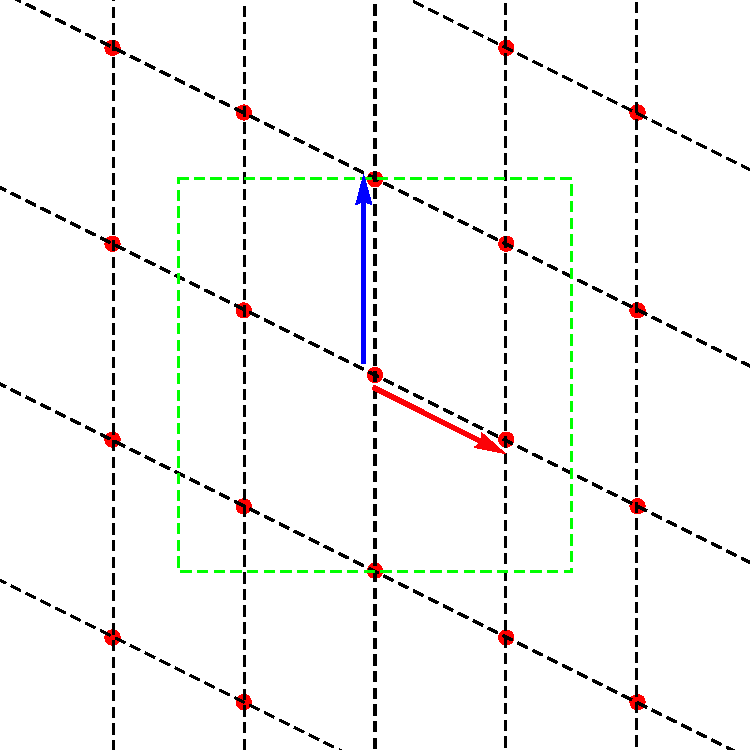
\includegraphics[width=0.40\textwidth]{HLReciprocalLattice1}
  \caption{\label{fig:HLReciprocalLattice}
%  (Color online)
(b)
    The reciprocal lattice \refeq{ReciprLattBasis}. Each reciprocal
    lattice point is a wave vector of the eigenvector of the translation
    operator with periodicity given by the Bravais lattice. The green
    dashed square encloses the first Brillouin zone of the {\em square
    lattice} (not the Bravais lattice). The wave vectors in the
    first Brillouin zone give all eigenvectors of the translation
    operator. Any wave vector outside of the first Brillouin zone is
    equivalent to a wave vector within it.
}
\end{figure}
%%%%%%%%%%%%%%%%%%%%%%%%%%%%%%%%%%%%%%%%%%%%%%%%%%%%%%%%%%%%%%%

    \PCpost {2019-09-11}{
Perhaps - if that helps:
copy to here the nomenclature used in \emph{PHYS-7143-19 week8}.
    }

    \PCpost{2019-11-24}{
    Do you have a closed form formula for counting these?
    We will need to include it in the paper. My
    $[2\!\times\!2]$ count
\(36 =
9+8+7+\cdots+1
\)
    was wrong.}

    \PCpost{2018-12-01}{ % 2020-01-11}{
Keep it as elementary as possible. Look at the beginning of the
\HREF{https://en.wikipedia.org/wiki/Chebyshev_polynomials} {wiki} - you can
already see our zeta function there. We need none of these funky trigonometric functions,
we only need the recurrence relations - they either already in this wiki, or in blogCats.tex,
or referred to in blogCats.tex.
    }

%\HLpost{2018-12-06}{
%I have a different way to prove \refeq{TableOfISP13952-2}. By the definition of the Chebyshev polynomials of the first kind:
%$\cos(n \theta) = T_n(\cos \theta)$, we can see that:
%\[
%T_\period{}\left[\cos\left(\frac{2 \pi j}{\period{}}\right)\right] = \cos(2\pi j) = 1 \, .
%\]
%So $\cos(2 \pi j /\period{})$, $j=0,1,...,\period{}-1$ are the roots of equation:
%\[
%T_n(x)-1=0 \, .
%\]
%So we have the identity:
%\beq
%T_n(x)-1 = 2^{\period{}-1} \prod_{j=0}^{\period{}-1} \left[x - \cos\left(\frac{2 \pi j }{\period{}}\right) \right]
%\, .
%\label{ProductToChebyshev}
%\eeq
%There is a coefficient $2^{\period{}-1}$ because the leading term in $T_n(x)$ is $2^{\period{}-1} x^\period{}$. Let $x=s/2$, and multiply both sides by 2, \refeq{ProductToChebyshev} becomes:
%\beq
%2T_n(s/2) - 2 = \prod_{j=0}^{\period{}-1} \left[s - 2\cos\left(\frac{2 \pi j }{\period{}}\right) \right]
%\, .
%\label{ProductToChebyshev-2}
%\eeq
%}

%%%%%%%%%%%%%%%%%%%%%%%%%%%%%%%%%%%%%%%%%%%%%%%%%%%%%%%%%%%%%
\begin{figure}
  \centering
(a)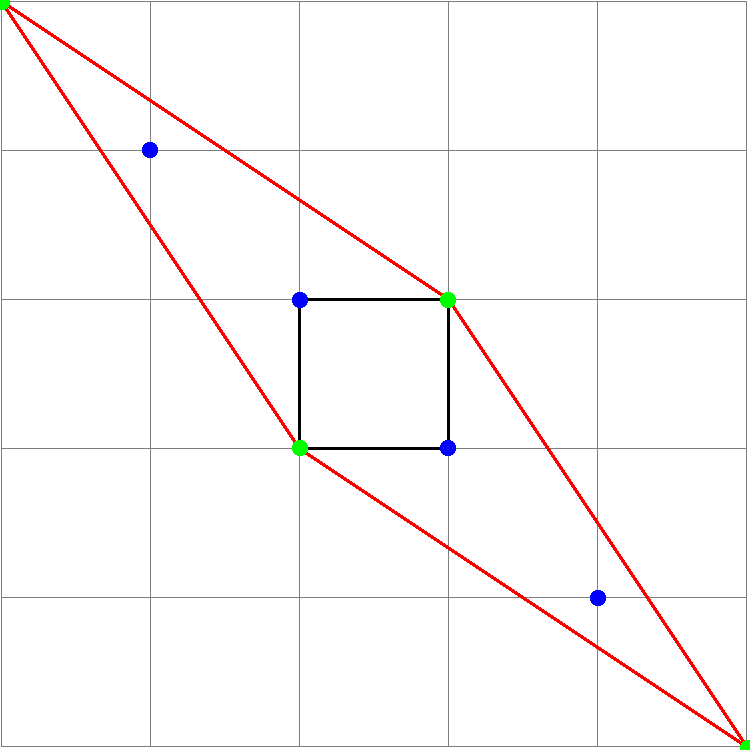
\includegraphics[width=0.45\textwidth]{HLLength2Counting}
(b)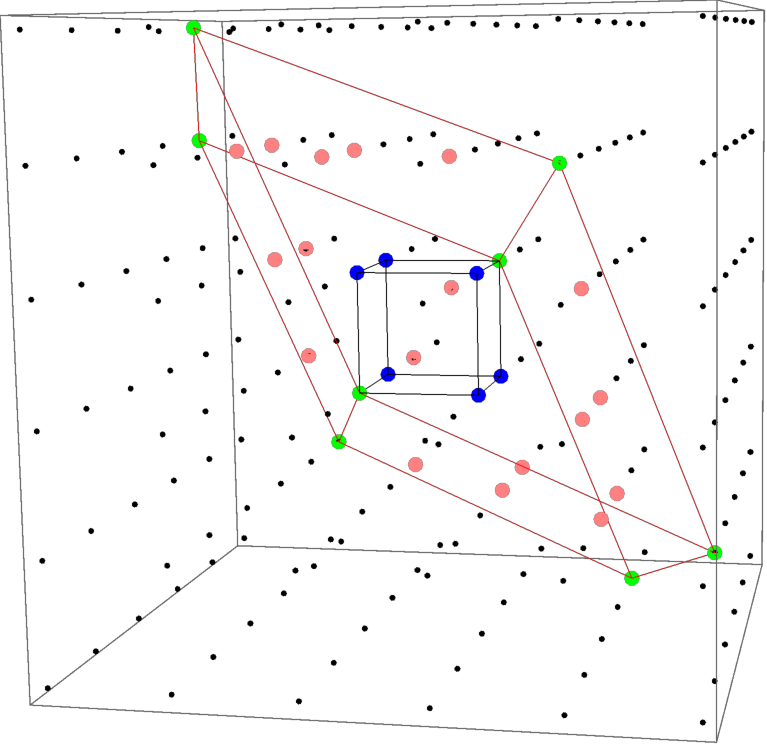
\includegraphics[width=0.45\textwidth]{HLLength3Counting-7210}
  \caption{\label{fig:HLCountingFigures}
(a) A 2-dimensional torus (with black border) stretched by $\jMorb$.
    The {\color{blue} blue} dots are internal integer points in the
    {\fundPip} (with red border). The {\color{green} green}
    dots are on the vertices of the {\fundPip}.
(b) A 3-dimensional torus (with black border) stretched by $\jMorb$.
    The {\color{blue} blue} dots are internal integer points in the
    stretched {\fundPip} (with red border). The {\color{green} green}
    dots are on the vertices of the {\fundPip}. The {
    pink} dots are on the surface of the {\fundPip}.
}
\end{figure}
%%%%%%%%%%%%%%%%%%%%%%%%%%%%%%%%%%%%%%%%%%%%%%%%%%%%%%%%%%%%%%%

%%%%%%%%%%%%%%%%%%%%%%%%%%%%%%%%%%%%%%%%%%%%%%%%%%%%%%%%%%%%%
% Predrag 2020-02-08 replaced Han's uneditable
% {HLLength2Counting}.pdf by catCyc2Jacob.svg
\begin{figure}
  \centering
(a)~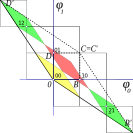
\includegraphics[width=0.35\textwidth]{catCyc2Jacob}
~~~
(b)~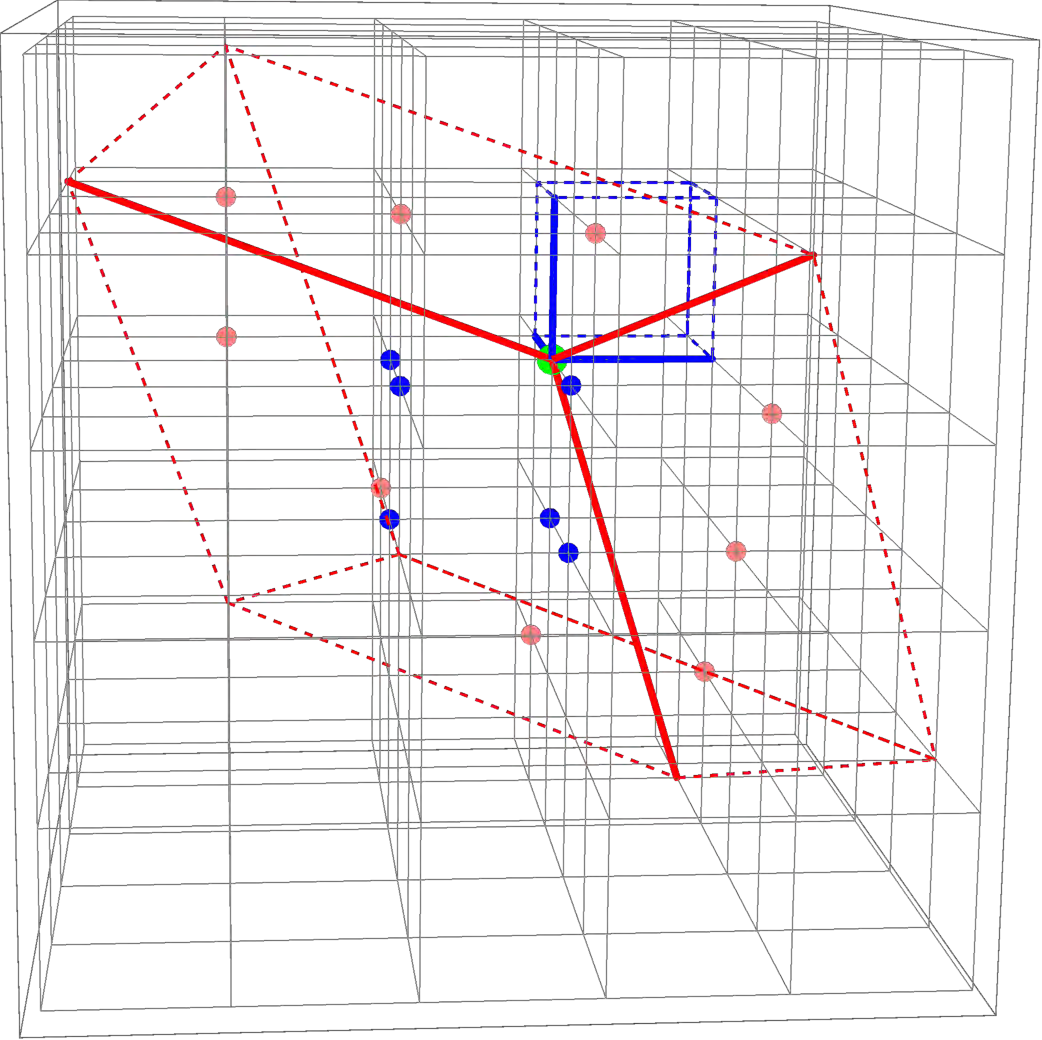
\includegraphics[width=0.40\textwidth]{HLLength3Counting}
  \caption{\label{fig:catCycJacobOld}
Was \reffig{fig:catCycJacob}, now superannuated:
(a)
    $[2\!\times\!2]$ {\jacobianOrb} $\jMorb$ \refeq{catFundPar2}
    had a wrong sign, meaningless partition into 9 rectangles.
(b) Han 2020-02-11: Intermediate attempt to draw \reffig{fig:catCycJacob}.
$[3\!\times\!3]$ {\jacobianOrb} $\jMorb$  had tons of irrelevant points plotted,
    is unintelligible.
}
\end{figure}
%%%%%%%%%%%%%%%%%%%%%%%%%%%%%%%%%%%%%%%%%%%%%%%%%%%%%%%%%%%%%%%

    \PCpost{2020-0131}{
Maybe if you plot only the points within (inside, and on the 3 faces
connected to the origin) the {\fundPip} of
\reffig{fig:catCycJacob}, no other integer points, it might be easier
to understand. Also, if you trace out the cubic lattice in light gray, it
will be clear the periodic points are on the integer lattice, in the
spirit of \reffig{fig:BernCyc2Jacob}\,(b).
    }

    \PCpost{2020-02-08}{
To Han: not writing up what you are working on in the blog is
self-defeating, as I cannot help you as long as I am not aware of you
doing anything. However, not saving figure-generating code in
\emph{siminos/mathematica} is also inefficient, as you are making me
regenerate all figures from scratch.
    }

    \PCpost{2018-06-21}{
Your difficulty is that you keep on thinking in Hamiltonian way, where
one steps in time, using the Hamilton's equations for $(q_t,p_t)$, where
we had replaced the momentum $p_t$ (at spatial position $\ell$) by
velocity $p_t=(\ssp_{\ell t}-\ssp_{\ell,t-1})/\Delta t$, and thus
initializing the Hamiltonian, a second-order difference equation for
\emph{evolution in time} by two horizontal rows $(\ssp_{\ell
t},\ssp_{\ell,t-1})\,,\;\ell\in\integers$ in the spacetime plane.

You have to think in the spacetime, Lagrangian way instead. On each
lattice site $z=(\ell,t)$ there is a scalar field $\ssp_{\ell t}$, not a
two-torus. The field $\ssp_{\ell,t-1}$ belongs to a neighboring site
$z=(\ell,t-1)$. The two fields do not form a dynamical system on a
two-torus, as the dynamics is also influenced by spatial neighbors
$\ssp_{\ell\pm1, t}$.
    }

\PCpost{2017-09-16}{
%%%%%%%%%%%%%%%%%%%%%%%%%%%%%%%%%%%%%%%%%%%%%%%%%%%%%%%%%%%%%%%%%%%%%%%%
Methods described above make it an easy task to obtain a
particular class of \twots\ for  the {\catlatt}.

\twoT's
coordinate representation $\Gamma=\{\ssp_z, z\in \ZLT\}$, is obtained by
taking inverse of \refeq{2dCoupledCats}:
  \begin{equation}
   \ssp_z=\sum_{z'\in \ZLT} \gp_{zz'} \Ssym{z'}, \qquad    \Ssym{z'}\in \Ai,
  \end{equation}
where $\gp_{zz'}$ is the corresponding Green's function with periodic
{\bcs}.
%%%%%%%%%%%%%%%%%%%%%%%%%%%%%%%%%%%%%%%%%%%%%%%%%%%%%%%%%%%%%%%%%%%%%%%%
    } %end \PCpost

    \PCpost{2018-12-01}{
Include here the song and dance from the remark.
    \\
    What Hill's formula? Is it
    \refeq{MacMei83(17)}? Not any longer sure that
     \rf{MacMei83} contains the Hill's formula...


discrete Hill's formula\rf{BolTre10}:
\beq
\det(\jMat_\Mm - \id) = \frac{(-1)^n \det \jMorb_\Mm}{\prod_{i=1}^n \det B_i}
\,,
\ee{BolTre10(2.8)a}
where for the one dimensional cat map the $B$ here is an $\BravCell{1}{1}{0}$ matrix:
\beq
B = - \frac{\delta^2 \genF[\ssp_{n+1},\ssp_{n}]}{\delta \ssp_{n+1} \delta \ssp_{n}} = 1
\,,
\ee{BolTre10(2.2)a}
    }


    \PCpost{2020-02-02}{
It is hard to find \refeq{LinearCatLatt} in {\GO}\rf{GutOsi15}. The paper
is mostly about the Hamiltonian formulation. Their (3.4) is the equation,
once on sets $c=d$ space-time isotropy, and drops their potential $V$.
Their perturbed equation (7.1) comes close to it. Their action (3.9) is a
bit mysterious as well.

Gutkin and Osipov\rf{GutOsi15}
refer to an \sPe\ \twot\ solution $p$ as a `many-particle periodic orbit', with
$\ssp_{n\zeit}$ `doubly-periodic', or `closed,'
\[
\ssp_{n\zeit} = \ssp_{n+\speriod{p},\zeit+\period{p}}
    \,,\quad
n = 0,1,2,\cdots, \speriod{p}-1
    \,;\quad
\zeit = 0,1,2,\cdots, \period{p}-1
    \,.
\]
    }

    \PCpost{2020-02-02}{
Note that in \refeq{catLatt} and throughout I have redefined the
stretching parameter ${s}$ to be stretching per dimension, \ie, ${s}$ in
\refeq{CatMap2d} is replaced by $d{s}$. This is consistent with
how one defines a diffusion constant on an isotropic $d$\dmn\ hypercubic
lattice.
    }

	\PCpost{2019-08-06}{% Is the lattice cell called the primitive cell?
    I do not think ``lattice cell'' is the standard terminology, and as
    you have chosen not to quotient the point group, what you have is not
    `primitive' - that would be 1/8th triangle that tiles the first
    Brillouin zone, I think. Please strictly follow the nomenclature of a
    single reference -presumably Dresselhaus \etal\rf{Dresselhaus07}, or
    Barvinok\rf{Barvinok08} or whatever  - and state so clearly in your
    text. Whenever you use a reference, ethics of the profession requires
    that you clearly cite it.
       }

    \HLpost{2020-02-20}{
\refFig{fig:HLfundPip2by1_1} is the \fundPip\ of a $[2\!\times\!1]_1$
\twot. The pattern of this periodic state is shown in \reffig{fig:2x1rpo}
(a). The \jacobianOrb\ of this \twot\ can be written as a
$[2\!\times\!2]$ matrix:
\[
    \jMorb
    =
     \left(\begin{array}{cc}
 -2s &  4 \\
  4 & -2s
 \end{array} \right) \, .
    \]
The shape of the \fundPip\ is very similar to \reffig{fig:catCycJacob} (a).
    }
%%%%%%%%%%%%%%%%%%%%%%%%%%%%%%%%%%%%%%%%%%%%%%%%%%%%%%%%%%%%%%%%%%
%\FIG{
\begin{figure}
  \centering
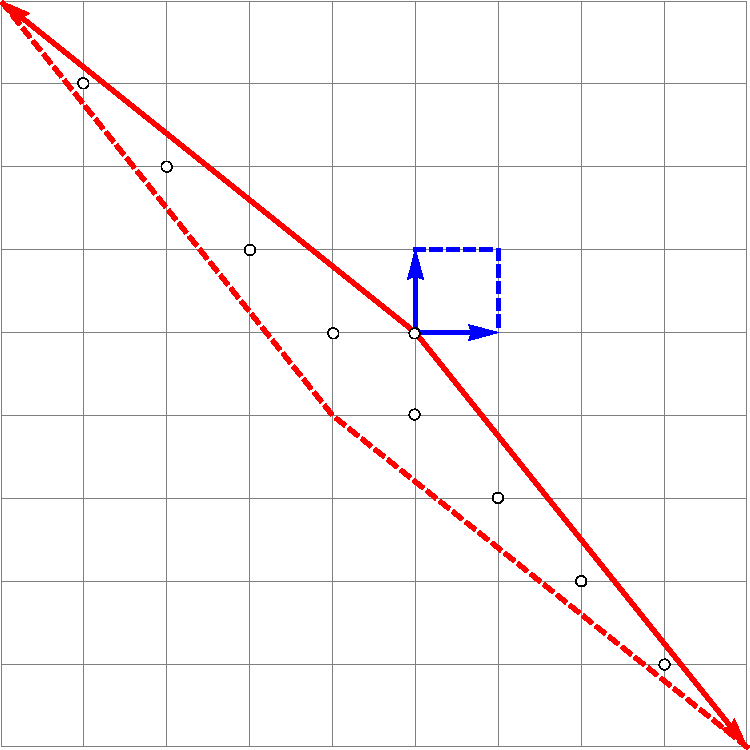
\includegraphics[width=0.40\textwidth]{HLfundPip2by1_1}
  \caption{\label{fig:HLfundPip2by1_1}
The \fundPip\ of a $[2\!\times\!1]_1$ \twot\ with $s=5/2$. Admissible field values lie within the unit square with blue boundaries. This unit square is stretched by the \jacobianOrb\ $\jMorb$ into the \fundPip\ with red boundaries. Integer points in the \fundPip\ are marked by the circles. There are 9 integer points in the \fundPip, in agreement with the counting formula.
            }
\end{figure}
%%%%%%%%%%%%%%%%%%%%%%%%%%%%%%%%%%%%%%%%%%%%%%%%%%%%%%%%%%%%%%%%%%

    \PCpost{2018-12-13}{
Must rethink the DIMENSION of $F[\Xx]$ and $\jMorb$. $F[\Xx]_i$
is a $\cl{}$\dmn\ vector function - is it dimensionally the same as
$\ssp_j$? Otherwise \jacobianOrb\ is not dimensionless, and cannot be
referred to as a `Jacobian'. Relation \refeq{detDet} only makes sense for
the dimensionless case. I think we are OK, but we have to be sure.
    }



    \PCpost{2019-08-11}{
to Han: this is wrong alphabet, for the
symmetric unit interval $\ssp\in[-1/2,1/2)$.
For all our examples we pick
the `least stretching' \catlatt\ with $s=5/2$,
with 9-letter alphabet
\beq
\A=\{\underline{4},\underline{3},\underline{2},\underline{1},
     0,1,2,3,4\}
\,.
\ee{catLattAlphabet}
    }

    \PCpost{2020-02-17}{
Now in \reftab{tab:LxTs}:
\bea
N_{\BravCell{1}{1}{0}}({s}) = 2({s}-2)
    \continue
N_{[2\!\times\!1]}({s}) = 4({s}-2)s
    \continue
N_{[2\!\times\!1]_1}({s}) = 4({s}-2)({s}+2)
    \continue
N_{[2\!\times\!2]}({s}) = 16({s}-2)s^2({s}+2)
    \continue
N_{\BravCell{3}{2}{0}}({s}) = 4({s}-2)s(2{s}-1)^2 (2{s}+3)^2
    \continue
N_{\BravCell{3}{2}{1}}({s}) = 64({s}-2){s}^3 ({s}+1)^2
    \continue
N_{\BravCell{3}{2}{2}}({s}) = 64({s}-2){s}^3 ({s}+1)^2
    \continue
N_{[3\!\times\!3]}({s}) = -32({s}-2)({s}+1)^4(2{s}-1)^4
\,.
\label{PC[LxT]volume}
\eea
    }

    \PCpost{2019-11-23}{Dropped:
For all our examples we pick
the `least stretching' hyperbolic \catlatt\ with $s=5$,
and restrict the
admissible field values $\ssp_{z}$ at lattice site $z=(n_1,n_2)$ to the
symmetric unit interval $\ssp\in[-1/2,1/2)$, with 9-letter alphabet
\refeq{catLattAlphabet}

the code depends on the choice of the unit interval:
the alphabet \A\ for $\ssp_{\zeit} \in [-1/2,1/2)$
differs from the alphabet for  $\ssp_{\zeit} \in [0,1)$.

Here $s=5/2$ and $\ssp_z\in[-1/2,1/2)$, so the
interior alphabet is one letter alphabet $\Ai=\{0\}$...

    }

%    \PCpost{2020-02-24}{
%Thanks for fixing \reftab{tab:LxTs=5/2} and \reftab{tab:LxTs}. Apparently
%I am not evaluating \emph{Tensors.nb} correctly - you'll show me how.
%    }


    \PCpost{2020-02-08}{
I think the $N_\cl{}=({s}-2)\cdots$ factorization is true for all $\cl{}$
in \refeq{1stChebGenF} and \reftab{tab:LxTs}. Do you understand it? Does
in the \templatt\ $s=2$ case, the Laplacian has a zero mode? A constant
$\ssp_i$ eigenvector? If so, why doesn't the \catlatt\ have
$N=({s}-2)^2\cdots$, one for each direction? Instead, one gets only a factor 2,
$N=2({s}-2)\cdots$.
    }

%    \PCpost{2020-02-24}{
%I had naively thought that $N_{\BravCell{\speriod{}}{1}{0}}$ families were
%the same as the 1\dmn\ \templatt\ \refeq{1stChebGenF}. Apparently not. Do
%you see something like a Chebyshev series here, or generating function
%similar to \refeq{Isola90-13}? If we cannot figure the bivariate zeta
%function, at least this family should work out?
%    }

    \PCpost{2020-02-24}{
Not urgent, but can you complete the primitive counts
$M_{[\speriod{}\!\times\!\period{}]_S}$ and decompositions of
$N_{[\speriod{}\!\times\!\period{}]_S}$ into primitive \twots\ in
\reftab{tab:LxTs=5/2} and perhaps also in \reftab{tab:LxTs}?
    }


    \PCpost{2020-03-05}{\tempLatt\ counting (all messed up,
    fix using \\ \emph{CatMaptopZeta.nb} output):
\bea
\sum_{{n}=0}^\infty N_{n} z^{n}
    & = & \frac{2-{s}z}{1 - s z + z^2}-\frac{2}{1 - z}
    \continue
\{N_{n}\} & = & s-2,s^2-4,
       s^3-3s-2,
        s^4-4s^2,
    \ceq
        2 \left(s^5-4 s^3+3 s\right)-s \left(s^4-3 s^2+1\right)-2,
    \ceq
        -2 \left(s^3-2s\right)-s\left(s^4-3 s^2+1\right)
    \ceq
-2 - s (-1 + 6 s^2 - 5 s^4 + s^6) + 2 (-4 s + 10 s^3 - 6 s^5 + s^7),
    \ceq
        -2s \left(s^5-4 s^3+3 s\right)-2 \left(s^4-3s^2+1\right)-2,
    \ceq
        -2 \left(s^5-4 s^3+3 s\right)
        +s \left(s^6-5 s^4+6s^2-1\right)-2,
        %s \left(s^7-6 s^5+10 s^3-4 s\right)-2 \left(s^6-5 s^4+6
%s^2-1\right)-2,-2 \left(s^7-6 s^5+10 s^3-4 s\right)+s \left(s^8-7 s^6+15
%s^4-10 s^2+1\right)-2,s \left(s^9-8 s^7+21 s^5-20 s^3+5 s\right)-2
%\left(s^8-7 s^6+15 s^4-10 s^2+1\right)-2,-2 \left(s^9-8 s^7+21 s^5-20
%s^3+5 s\right)+s \left(s^{10}-9 s^8+28 s^6-35 s^4+15 s^2-1\right)-2,s
%\left(s^{11}-10 s^9+36 s^7-56 s^5+35 s^3-6 s\right)-2 \left(s^{10}-9
%s^8+28 s^6-35 s^4+15 s^2-1\right)-2
\,,
\label{1stChebGenFdrop}
\eea
    }

     \PCpost{2020-03-23} {
Lot's of headless \KSe\ floundering in preparing \emph{BlogCats.tex}
\refsect{sect:KSe} saved below. Hopefully the resulting discretized \KSe\
\refeq{KSdiscr5} is correct...

\medskip

The discretized \KSe\ is of the form
\beq
\pde_\zeit \mathsf{U} + \frac{\alpha}{2}\pde_x\mathsf{U}^2
  - \beta\,\Laplacian_x \mathsf{U} + \gamma\,\Laplacian_x^2 \mathsf{U}
= 0
\,.
\ee{KSdiscr1}
Rescale $\mathsf{U}\to\mathsf{U}/\Delta\zeit$
%, divide by $\Delta x$:
\beq
\frac{\pde_\zeit}{\Delta\zeit}\mathsf{U}
+ \frac{(\Delta x)^2}{\Delta\zeit}\frac{\alpha}{2}\frac{\pde_x}{\Delta x}\mathsf{U}^2
  - \frac{(\Delta x)^2}{\Delta\zeit}\beta\,\frac{\Laplacian_x}{(\Delta x)^2} \mathsf{U}
  + \frac{(\Delta x)^4}{\Delta\zeit}\gamma\,\frac{\Laplacian_x^2}{(\Delta x)^4}\mathsf{U}
= 0
\,.
\ee{KSdiscr2}
Our canonical choice is setting these
\beq
\alpha=\frac{\Delta\zeit}{(\Delta x)^2}
    \,,\quad
\beta=-\frac{\Delta\zeit}{(\Delta x)^2}
    \,,\quad
\gamma=\frac{\Delta\zeit}{(\Delta x)^4}
\,,
\ee{KSscales}
equal to 1, parametrazing the problem with
$\speriod{}=1/\Delta x$, $\period{}=1/\Delta\zeit$,
\beq
\frac{1}{\period{}}\frac{\pde_\zeit}{\Delta\zeit} \mathsf{U}
  + \frac{1}{\speriod{}}\frac{\alpha}{2}\frac{\pde_x}{\Delta x}\mathsf{U}^2
  - \frac{1}{\speriod{}^2}\beta\,\frac{\Laplacian_x}{(\Delta x)^2} \mathsf{U}
  + \frac{1}{\speriod{}^4}\gamma\,\frac{\Laplacian_x^2}{(\Delta x)^4}\mathsf{U}
= 0
\,.
\ee{KSdiscr3}
Rescale $\mathsf{U}\to\mathsf{U}\,\period{}$
\beq
\frac{\pde_\zeit}{\Delta\zeit} \mathsf{U}
  + \frac{\period{}^2}{\speriod{}}\frac{\alpha}{2}\frac{\pde_x}{\Delta x}\mathsf{U}^2
  - \frac{\period{}}{\speriod{}^2}\beta\,\frac{\Laplacian_x}{(\Delta x)^2} \mathsf{U}
  + \frac{\period{}}{\speriod{}^4}\gamma\,\frac{\Laplacian_x^2}{(\Delta x)^4}\mathsf{U}
= 0
\,.
\ee{KSdiscr4}
Our canonical choice is setting these
\beq
\alpha=\speriod{}/\period{}^2
    \,,\quad
\beta=-\speriod{}^2/\period{}
    \,,\quad
\gamma=\speriod{}^4/\period{}
\,,
\ee{KSscales1}
equal to 1,
\beq
\frac{\pde_\zeit}{\Delta\zeit} \mathsf{U}
  + \frac{1}{2}\frac{\pde_x}{\Delta x}\mathsf{U}^2
  + \frac{\Laplacian_x}{(\Delta x)^2} \mathsf{U}
  + \left(\frac{\Laplacian_x}{(\Delta x)^2}\right)^2\mathsf{U}
= 0
\,,
\ee{KSdiscr6}
    }

%    \PCpost{2020-02-24}{
% Priority \# 1: {\em appeFourier.tex}.
%    }

    \PCpost{2019-12-28}{
My argument along the following lines was unnecessarily complicated:
%where we have used
\beq
%\sum_{k=0}^{\cl{}-1} \epsilon^{k} = 0 \,,\qquad
\epsilon^0\epsilon^1\epsilon^2\cdots\epsilon^{\cl{}\!-\!1}=1
\,.
\ee{circKron}
can be eliminated by going from products
to sums over cyclic eigenvalues. For example, if
a polynomial is of form
\(
G(x)/(x-\lambda_0)
\,,
\)
with the zeroth root
\(
(x-\epsilon^0)= (x-1)
\)
quotiented out from the characteristic polynomial, % \refeq{CNcharPoly},
\[
\frac{x^N-1}{x-1}
=
(x-\epsilon)(x-\epsilon^2)\cdots(x-\epsilon^{N-1})
\,.
\]
Consider a sum of the first $N$ terms of a geometric series,
multiplied by $(x-1)/(x-1)$:
\beq
1+x+\cdots + x^{N-1}
=
\sum_{m=0}^{N-1} x^m
=
\frac{1}{x-1} \sum_{m=0}^{N-1} (x-1)\,x^m
=
\frac{x^N-1}{x-1}
\,.
\ee{BG:PartSum}
So, the products can be written as sums
\beq
(x-\epsilon)(x-\epsilon^2)\cdots(x-\epsilon^{N-1})
=
1+x+\cdots + x^{N-1}
\,.
\ee{BG:PartSum1}
In \Cn{N} $P_n$ projection operators, the denominators are
evaluated by substituting $x\to1$ into \refeq{BG:PartSum1}; that adds up
to $N$.
The numerator is evaluated by substituting $x\to\epsilon^{-n} M$.
We obtain the projection operator as a discrete Fourier weighted sum
of matrices $M^m$,
\beq
P_n=\frac{1}{N}\sum_{m=0}^{N-1}e^{-i\,\frac{2\pi}{N}nm}\,M^m
\,,
\ee{examDisFourT}
instead of the usual product form.
    }

    \PCpost{2020-06-08}{dropped:
The periodicity of a {\lattstate}s is described by the $d$\dmn\ Bravais lattice:
\beq
\Lambda =
\left\{ \sum_{i=1}^d n_i \mathbf{a}_i\,|\,n_i \in \mathbb{Z}\right\} \, .
\ee{dDBravaisLattice}

The {\jacobianOrb} \refeq{catlattFix} is constructed from $d$ commuting
translation operators $\shift_{i}$ with $i=1, \dots, d$. The eigenvectors of these translation
operators are plane waves:
 \beq
f_{k}({z}) = e^{i {k} \cdot {z}}
\,,
\ee{PlaneWave}
where $\mathbf{k}$ is a $d$\dmn\ wave vector. A general plane wave does not
satisfy the periodicity \refeq{dDPeriodicCondition}, unless
\beq
e^{i {k} \cdot {R}} = 1
\, .
\ee{PeriodicPlaneWave}
Since ${R}$ is a vector from the Bravais lattice $\lattice$, the wave
vector $\mathbf{k}$ must lie in the reciprocal lattice of $\Lambda$:
\beq
\mathbf{k} \in \Lambda^*
\,,\quad
\Lambda^* =
\left\{ \sum_{i=1}^d m_i \mathbf{b}_i\,|\,m_i \in \mathbb{Z}\right\} \, ,
\ee{dDReciprocalLattice}
where the primitive reciprocal lattice vectors $\mathbf{b}_i$ satisfy:
 \beq
\mathbf{b}_i \cdot \mathbf{a}_j = 2 \pi \delta_{ij} \, .
\ee{ReciprLattBasis}
To get the eigenvectors and the corresponding eigenvalues
of the \jacobianOrb, note that
\beq
(\shift_j + \shift_{j}^{-1}) e^{i {k} \cdot {z}}
=
e^{i ({k} \cdot {z} - k_j)} + e^{i ({k} \cdot {z} + k_j)}
=
(2 \cos k_j) e^{i {k} \cdot {z}} \, ,
\ee{EigenvalueTranslation}
where the $\mathbf{k}=(k_1,k_2,\cdots,k_d)$. Hence the eigenvalue of the
{\jacobianOrb} \refeq{catlattFix} corresponding to the eigenvector with
the wave vector $\mathbf{k}$ \refeq{PlaneWave} is
\beq
\lambda_{k} = \sum_{j=1}^d \left( 2\cos k_j - s \right)
\,.
\ee{dDEigenvalue}
and compute
its inverse, the Green's function.
\bigskip

The generalization to $d$ \spt\ dimensions is immediate.
A periodic {{\lattstate}} ${\Xx}=\{\ssp_z\}$, $z\in\integers^d$ is
a {point} within the $(\ell_1\ell_2\cdots\ell_d)$\dmn\
unit hyper-cube $[0,1)^{\ell_1\ell_2\cdots\ell_d}$, where $\ell_j$
is the lattice period in direction $j$, and the
$(\ell_1\ell_2\cdots\ell_d)^2$\dmn\ {\jacobianOrb} $\jMorb_{zz'}$ is
given by
\beq
\jMorb = \sum_{j=1}^{d}\left(\shift_j-{s}\id+\shift_{j}^{-1}\right)
\,.
\ee{catlattFixover}
Here $\shift_i$ is a {\shiftOp}
\refeq{hopMatrix} which translates the field in the $i$th
direction by one lattice spacing. Its inverse $\shift_{i}^{-1}$
translates the field in the negative $i$th direction.


From now on we specialize to the 2\dmn, $z=(n,\zeit)\in\integers^2$
\spt\ lattice, and replace the $(\ell_1,\ell_2)$ notation for lattice
periods by $(\speriod{},\period{})$, where $\speriod{}$ is the `spatial',
and $\period{}$ the `temporal' lattice period. The field $\ssp_i$
takes values in the $\speriod{}\period{}$\dmn\ unit hyper-cube
$\Xx\in[0,1)^{\speriod{}\period{}}$.

Throw away all {\brick}s which are repeats of
shorter {\brick}s in the temporal direction. What
remains in $N_k$ prime periodic \brick s $p$ of the same size
$[\speriod{p}\times\period{p}]=[\speriod{k}\times\period{k}]$.

This is essential to all that follows, as the Lagrangian formulation will
apply to \catlatt\ in any number of spatial dimensions as well.

  }

\PCpost{2020-05-31} {
  {\em Periodic
orbits in coupled {H{\'e}non} maps: {Lyapunov} and multifractal analysis}
is quite close to our \catlatt. The problem is harder,
as the {H{\'e}non} map is nonlinear.
    }



    \PCpost{2020-05-28}{
    Track this down:
Vicky Weiskopf: ``It is better to uncover a little than cover a lot''
    }
\end{description}

\subsection{Hill's formula:
             stability of an orbit vs. its time-evolution stability}

{\bf 2020-07-14 Han}

To prove the Hill's formula \refeq{detDetCat} for the cat map, first note
that both the left hand side and right hand side are polynomials with the
same leading terms $s^\cl{}$. The left hand side is the determinant of
the tri-diagonal Toeplitz matrix \refeq{Hessian}.  From the
\refeq{StabMtlpr} and \refeq{noPerPts}, the right hand side can be
written in the form  %\label{Isola90-13}
\bea
|\det(\jMat^{\cl{}} - \id)|
          &=& \ExpaEig^{\cl{}} + \ExpaEig^{-\cl{}} - 2 \continue
          &=& 2 \cosh( \cl{} \Lyap) -2 \continue
          &=& 2 \cosh \left[ \cl{} \textrm{arc}\cosh\left(\frac{s}{2}\right)\right] -2
          \,,
\label{HillsForR}
\eea
where we used $s=2\cosh(\Lyap)$. As the Chebyshev polynomial of
the first kind can be written as $T_\cl{}(x) = \cosh [ \cl{}
\textrm{arc}\cosh(x)]$, the right hand side of \refeq{detDetCat} is
\[
|\det(\jMat^{\cl{}} - \id)|
=
2 T_\cl{}\left(\frac{s}{2}\right)-2 \, ,
\]
which has the leading term $s^\cl{}$.

Let $u = (u_j)_{j = 1, 2, \dots, \cl{}}$ be the variation to the periodic
orbit $\Xx$ with length $\cl{}$. $\jMorb u = 0$ only if $\jMat^\cl{} w =
w$ where $w=(u_1,u_2)$. Then $|\det(\jMat^{\cl{}} - \id)|=0$ is
equivalent to $|\Det\jMorb|=0$. Then the polynomials $|\Det\jMorb|$
and $|\det(\jMat^{\cl{}} - \id)|$ have the same roots and the same
leading terms so they are equal.

{\bf 2020-07-17 Han}

Let $s$ go to infinity. Then the stability multipliers becomes:
\bea
\lim_{s \to \infty} \ExpaEig = \lim_{s \to \infty} \frac{s+\sqrt{s^2-4}}{2} = s \, , \continue
\lim_{s \to \infty} \ExpaEig^{-1} = \lim_{s \to \infty} \frac{2}{s+\sqrt{s^2-4}} = \lim_{s \to \infty} \frac{1}{s} =0 \, .
\label{StabMtlprLimit}
\eea
Then in the limit:
\beq
\lim_{s \to \infty} |\det(\jMat^{\cl{}} - \id)|
          = \lim_{s \to \infty} \ExpaEig^{\cl{}} + \ExpaEig^{-\cl{}} - 2
          = s^\cl{}
          \,,
\ee{HillsForRightLimit}
So the leading term of the right hand side of \refeq{detDetCat} is $s^\cl{}$.

\bea
|\det(\jMat^{\cl{}} - \id)|
          &=& \ExpaEig^{\cl{}} + \ExpaEig^{-\cl{}} - 2 \continue
          &=& \left(\frac{s+\sqrt{s^2-4}}{2}\right)^\cl{} + \left(\frac{s-\sqrt{s^2-4}}{2}\right)^\cl{} -2 \continue
          &=& \frac{1}{2^\cl{}} \sum_{k=0}^{\frac{\cl{}}{2}} {2k \choose \cl{}} s^{\cl{}-2k}(s^2-4)^k - 2
          \,,
\label{HillsForRight}
\eea

{\bf 2020-07-21 Han}
The \jacobianOrb\ of the \templatt\ has form:
\[
\jMorb
=
\left(
\begin{array}{cccc}
 -s & 1 & 0 & 1 \\
 1 & -s & 1 & 0 \\
 0 & 1 & -s & 1 \\
 1 & 0 & 1 & -s \\
\end{array}
\right)
\, ,
\]
while the \jacobianOrb\ from \refeq{bernNotHill} is
\[
\jMorb'=\id- \shift^{-1} \otimes \jMat
=
\left(
\begin{array}{cc|cc|cc|cc}
 1 & 0 & 0 & 0 & 0 & 0 & 0 & -1 \\
 0 & 1 & 0 & 0 & 0 & 0 & 1 & -s \\ \hline
 0 & -1 & 1 & 0 & 0 & 0 & 0 & 0 \\
 1 & -s & 0 & 1 & 0 & 0 & 0 & 0 \\ \hline
 0 & 0 & 0 & -1 & 1 & 0 & 0 & 0 \\
 0 & 0 & 1 & -s & 0 & 1 & 0 & 0 \\ \hline
 0 & 0 & 0 & 0 & 0 & -1 & 1 & 0 \\
 0 & 0 & 0 & 0 & 1 & -s & 0 & 1 \\
\end{array}
\right)
\, .
\]
We know that
\[
\det \left( \id- \shift^{-1} \otimes \jMat \right)
=
\det \left( \id-\jMat \otimes \shift^{-1} \right)
=
\det \left[\left( \id-\jMat \otimes \shift^{-1} \right) \left( \id_{[2\times 2]} \otimes \shift \right)\right]
\, ,
\]
where
\[
\id-\jMat \otimes \shift^{-1}
=
\left(
\begin{array}{cccc|cccc}
 1 & 0 & 0 & 0 & 0 & 0 & 0 & -1 \\
 0 & 1 & 0 & 0 & -1 & 0 & 0 & 0 \\
 0 & 0 & 1 & 0 & 0 & -1 & 0 & 0 \\
 0 & 0 & 0 & 1 & 0 & 0 & -1 & 0 \\ \hline
 0 & 0 & 0 & 1 & 1 & 0 & 0 & -s \\
 1 & 0 & 0 & 0 & -s & 1 & 0 & 0 \\
 0 & 1 & 0 & 0 & 0 & -s & 1 & 0 \\
 0 & 0 & 1 & 0 & 0 & 0 & -s & 1 \\
\end{array}
\right)
\, ,
\]
and
\[
\left( \id-\jMat \otimes \shift^{-1} \right) \left( \id_{[2\times 2]} \otimes \shift \right)
=
\left(
\begin{array}{cccc|cccc}
 0 & 1 & 0 & 0 & -1 & 0 & 0 & 0 \\
 0 & 0 & 1 & 0 & 0 & -1 & 0 & 0 \\
 0 & 0 & 0 & 1 & 0 & 0 & -1 & 0 \\
 1 & 0 & 0 & 0 & 0 & 0 & 0 & -1 \\ \hline
 1 & 0 & 0 & 0 & -s & 1 & 0 & 0 \\
 0 & 1 & 0 & 0 & 0 & -s & 1 & 0 \\
 0 & 0 & 1 & 0 & 0 & 0 & -s & 1 \\
 0 & 0 & 0 & 1 & 1 & 0 & 0 & -s \\
\end{array}
\right)
\,.
\]
The determinant of a block matrix is
\[
\det
\left(
\begin{array}{cc}
A & B \\
C & D \\
\end{array}
\right)
=
\det(A)\det(D-CA^{-1}B)
\, .
\]
Then we have:
\[
\det \left[\left( \id-\jMat \otimes \shift^{-1} \right) \left( \id_{[2\times 2]} \otimes \shift \right)\right]
=
\det [-s \id + \shift - \id \shift^{-1} (-\id)]
=
\det \jMorb
\,.
\]


What happens if we change the order of how we block the matrix, and
consider ${\mathbf{\jMat}_1} \otimes \shift_2^{-1}$ instead of
$\shift_2^{-1}\otimes{\mathbf{\jMat}_1}$ in \refeq{eq:orbitJPVtempJ}?

In particular, by similarity relation \refeq{wikiKron3},
\refeq{eq:orbitJPVtempJ} is equivalent to ...

\begin{description}
    \PCpost{2020-07-25} {
%\subsection{\catLatt\ Hill's formula leftovers}
%\label{sect:catlattHillover}
%Not used in {\em CL18}:




\bigskip\bigskip



using
\beq
\det
\left(
\begin{array}{cc}
A & B \\
C & D \\
\end{array}
\right)
=
\det(D)\,\det(A-BD^{-1}C)
\,.
\ee{det2x2blockMat1}
so (not rechecked),
\bea
\det(1-\mathbf{\jMat} \otimes \shift^{-1})
    &=&
\det
 \left[\begin{array}{cc}
\id_1 & -\id_1\\
\id_1 & {\id_1+\mathbf{\jMorb}_1}
\end{array}
\right]
=
\det({2\id_1+\mathbf{\jMorb}_1})\,\det(\id_1)
%\det [- 2(s-1)\id + \shift - \id \shift^{-1} (-\id)] =
    \continue
    &=&
\det [\shift - 2(s-1)\id + \shift^{-1}]
    =
|\det \jMorb |
\,.
\label{det2x2blockMat2}
\eea

in time with a [$2\speriod{}\!\times\!2\speriod{}$] block matrix
$\hat{\mathbf{\jMat}}$,
    \PC{2020-07-15}{
    Rewriting here \refeq{HLpartition2d}, \refeq{HLpartition2d2} as
    \refeq{CatMap2dHill}; will use $\mathsf{U}$ for the variation of \Xx.
    }
\bea
\hat{\Xx}_{\zeit+1} &=&
  \hat{\mathbf{\jMat}} \hat{\Xx}_\zeit - \hat{\mathsf{\Ssym{}}}_\zeit
\,,\qquad %\continue
\hat{\mathbf{\jMat}}  =
 \left[\begin{array}{cc}
{\bf 0} & {\bf I}\\
{\bf -I} & {-{\bf \jMorb}_\zeit}
 \end{array} \right]
 \,.
\label{HLpartition2d_Hill}
\eea

The \HREF{https://en.wikipedia.org/wiki/Kronecker_product} {Kronecker
product} $\mathbf{A}\otimes\mathbf{B}$ is an operation by [$m\times n$]
matrix $\mathbf{A}$ on [$p\times q$] matrix $\mathbf{B}$, resulting in an
[$pm\times qn$] block matrix:
\beq
\mathbf{A}\otimes\mathbf{B} =
\left(\begin{array}{ccc} %\begin{bmatrix}
  a_{11} \mathbf{B} & \cdots & a_{1n}\mathbf{B} \\
             \vdots & \ddots &           \vdots \\
  a_{m1} \mathbf{B} & \cdots & a_{mn} \mathbf{B}
\end{array}\right) %\end{bmatrix}
\,,
\ee{KroneckerProdover}

\beq
\tr(\mathbf {A} \otimes \mathbf {B} )
=\tr\mathbf {A} \,\tr\mathbf {B} \quad\mbox{and}\quad \det(\mathbf {A} \otimes \mathbf {B} )=(\det \mathbf {A} )^{m}(\det \mathbf {B} )^{n}
\,.
\ee{wikiKron2over}

$\mathbf{\jMorb}_1$ is the spatial $[\speriod{}\!\times\!\speriod{}]$
{\jacobianOrb} of  form (XX),
\bea
\mathbf{\jMorb}_1
        &=&
\shift_{1}^{-1} - 2s \id_1 + \shift_{1}
        \continue
        &=&
\left(\begin{array}{cccccc}
 -{2s}& 1 & 0 & \dots   & 1 \\
 1 &  -{2s}& 1 & \dots  & 0 \\
\vdots & \vdots &\vdots &\ddots &\vdots\\
 1 & 0 & \dots & 1      & -{2s}
        \end{array} \right)
\,.
\label{Hessian_Hillover}
\eea

If $\mathbf{A}$, $\mathbf{B}$, $\mathbf{C}$ and $\mathbf{D}$ are matrices
of such size that one can form the matrix products $\mathbf{AC}$ and
$\mathbf{BD}$, then the product of two block matrices is
a block matrix:
\beq
(\mathbf{A}\otimes\mathbf{B})\,(\mathbf{C}\otimes\mathbf{D})
%= (\mathbf{A}\mathbf{C})\otimes(\mathbf{B}\mathbf{D})
%  {\displaystyle (\mathbf {A} \otimes \mathbf {B} )(\mathbf {C} \otimes \mathbf {D} )
  =(\mathbf{AC})\otimes (\mathbf{BD})
  \,.
\ee{mixedProdover}

If $\lambda _{1}, ..., \lambda _{n}$ are the eigenvalues of $\mathbf{A}$,
and $\mu_{1}, ..., \mu_{m}$ the eigenvalues of $\mathbf{B}$, then the
eigenvalues of $\mathbf{A}\otimes\mathbf{B}$ are
\beq
\lambda_{i}\mu_{j},\qquad i=1,\ldots ,n,\,j=1,\ldots ,m
\,,
\ee{wikiKron1}

temporal {\jacobian} matrix %$\mathbf{\jMat}$
\beq
 \mathbf{\jMat}
=
 \left(\begin{array}{cc}
 0 & 1 \\
 -1 & s
 \end{array} \right)
% +
% \left(\begin{array}{cc}
% 0 & 0 \\
% 0 & s
% \end{array} \right)
 =
 \omega
    \left(
 \id
 -
 \omega
 \left(\begin{array}{cc}
 0 & 0 \\
 0 & s
 \end{array} \right)
    \right)
\,.
\ee{eq:StateSpCatMap_Hillover}

\bea
\hat{\Xx}_{\zeit+1} &=&
  \jMat_{PV} \hat{\Xx}_\zeit - \hat{\mathsf{\Ssym{}}}_\zeit
    \continue
\jMat_{PV} &=&
 \left[\begin{array}{cc}
{\bf 0} & {\bf I}\\
{\bf -I} & {-{\bf \jMorb}_\zeit}
 \end{array} \right]
            =
{\omega} -
 \left[\begin{array}{cc}
{\bf 0} & {\bf 0}\\
{\bf 0} & {{\bf \jMorb}_\zeit}
 \end{array} \right]
\label{HLpartition2d_Hillover}
\eea
 as
a generalization of the $\speriod{}=1$ cat map \refeq{PV2config},
where
\beq
{\omega} =  \left[\begin{array}{cc}
{\bf 0} & {\bf I}\\
-{\bf I} & {~\bf 0}
 \end{array} \right]
	\,,
\ee{symplNormConvover}
is an antisymmetric  [$2\speriod{}\!\times\!2\speriod{}$] matrix,
$\omega^2=-\id$,
    }

    \PCpost{2019-11-23}{
For uses of the lexical ordering, ChaosBook table
\toChaosBook{section.18.2}
{18.1:} {\em {\Orbit}s for the binary symbolic dynamics up to length 9},
and appendix
\toChaosBook{section.R.2}
{A18.2} {\em Prime factorization for dynamical itineraries}
might be of interest.

In the paper, we will probably first review the \templatt\ counting,
something along the lines of the above tables.

suggestion of
constructing covering prime \brick s wildly overcounts the candidates for
\admissible\ prime \twots, so we should give up this avenue of
constructing them - no need to count any larger Bravais lattices.
    }

    \PCpost{2019-08-11}{to Han - we need something like \\
For the $s=5/2$ example at hand, \refeq{2DCountingFormula} yields the
numbers of relative prime \twots\ $\BravCell{\speriod{}}{1}{1}$
\beq
\{M_{\BravCell{\speriod{}}{1}{0}}\}
= (M_{\BravCell{1}{1}{0}},M_{2\!\times\!1},M_{3\!\times\!1},\cdots)
=(1,9,?,?,?,\cdots)
\,,
\ee{noTwotsnx1s=5}
to be contrasted with \templatt\ counting \refeq{noPrimeCycs=3},
this time for $s=3$,
\beq
\{M_{\speriod{}}\} = (M_1,M_2,M_3,M_4,M_5,\cdots)
=(1,?,?,?,?,\cdots)
\,.
\ee{noPrimeCycs=5}
    }

    \HLpost{2019-11-24}{
A brute way to determine the {\em \admissible} \brick s, is to compute $\Xx_p$ for each
prime \brick\ $\Mm_p$, and eliminate every $\Xx_p$ which contains a
lattice site or sites on which the value of the field violates the
admissibility condition $\ssp_z\in[0,1)^2$.

The interior alphabet depends on the value of $s$ and the \admissible\
range of $\ssp_z$.
For $s=5/2$, $\ssp_z\in[0,1)$, the interior alphabet is
$\Ai=\{0,1\}$ (see eq.~(38) in \refref{GHJSC16}).
For $s=7/2$, $\ssp_z\in[0,1)$, the interior alphabet is
$\Ai=\{0,1,2,3\}$ (eq.~(46) in \refref{GHJSC16}).
    }

    \PCpost{2020-09-06}{
Removed the Mathematica expansion of \refeq{1stChebGenF}
\bea
\sum_{{n}=0}^\infty N_{n} z^{n}
    & = & \frac{2-{s}z}{1 - s z + z^2}-\frac{2}{1 - z}
    \continue
& = & (s-2)\left[z + ({s}+2) z^2 + ({s}+1)^2 z^3 \right.
    \ceq
      \left.\qquad\quad
      +\,({s}+2)\,{s}^2 z^4 + (s^2+ s-1)^2 z^5  +  \cdots\right]
\,,
\label{blog1stChebGenF}
\eea

\(
s-2,s^2-4,
       s^3-3s-2,
        s^4-4s^2,
        -2 \left(s^3-2s\right)+s\left(s^4-3 s^2+1\right)-2,
\)

\(
        s \left(s^5-4 s^3+3 s\right)-2 \left(s^4-3s^2+1\right)-2,
        -2 \left(s^5-4 s^3+3 s\right)+s \left(s^6-5 s^4+6s^2-1\right)-2,
        %s \left(s^7-6 s^5+10 s^3-4 s\right)-2 \left(s^6-5 s^4+6
%s^2-1\right)-2,-2 \left(s^7-6 s^5+10 s^3-4 s\right)+s \left(s^8-7 s^6+15
%s^4-10 s^2+1\right)-2,s \left(s^9-8 s^7+21 s^5-20 s^3+5 s\right)-2
%\left(s^8-7 s^6+15 s^4-10 s^2+1\right)-2,-2 \left(s^9-8 s^7+21 s^5-20
%s^3+5 s\right)+s \left(s^{10}-9 s^8+28 s^6-35 s^4+15 s^2-1\right)-2,s
%\left(s^{11}-10 s^9+36 s^7-56 s^5+35 s^3-6 s\right)-2 \left(s^{10}-9
%s^8+28 s^6-35 s^4+15 s^2-1\right)-2
\)
    }

%%%%%%%%%%%%%%%%%%%%%%%%%%%%%%%%%%%%%%%%%%%%%%%%%%%%%%%%%%%%%%%%%%%%%%%%
    \BGpost{2016-11-01} {
{\bf ``Deeper insight'' into $d=2$ symbolic dynamics}:
Relevance to semiclassics.

``Classical foundations of many-particle
quantum chaos'' I believe could become a game-changer
    }
%%%%%%%%%%%%%%%%%%%%%%%%%%%%%%%%%%%%%%%%%%%%%%%%%%%%%%%%%%%%%%%%%%%%%%%%

    \PCpost{2016-12-24}{``
Alternatively, one can consider the dynamics on the
infinite line, and interpret $\Ssym{\zeit}$ as a jump to $\Ssym{\zeit}$th interval. This
leads to the phenomenon of ``deterministic diffusion''\rf{GroFuj82,ScFrKa82},
and its \po\ theory\rf{art91,CGS92}, with unit circle \po s in one-to-one
relation to the relative periodic (``running'') orbits on the line, and
symbolic dynamics given by $\Ssym{\zeit}$'s.

For single-parameter, 1\dmn\
sawtooth maps, it is possible to find infinitely many values of the parameter
such that the grammar is finite (a finite subshift), and the exact diffusion
constant is given by a finite-polynomial \tzeta\rf{CBdiffusion}. For cat maps, deterministic diffusion constants
are not known exactly\rf{ArtStr97}.
''  }

    \PCedit{2020-07-15}{
Perhaps refer to ChaosBook
\toChaosBook{section.8.1}
{8.1 Hamiltonian flows}, when discussing `two-configuration' form \refeq{PV2config}.
    }

    \PCpost{2020-09-19}{
dropped from the abstract: ``, with the {\lattstate} and its symbolic encoding related linearly.''
\bigskip

dropped: ``the problem of enumerating and determining all global
solutions stripped to its bare essentials.''

As a function of the strengths of cell-cell couplings, dynamics can exhibit rich
phase-transitions structure\rf{Kaneko84}. In this paper we chose couplings such
that the system is fully turbulent.

``For an explicit example, see \refsect{s:catLattRel3x2}.''

Hamiltonan, so symplectic or area preserving, but that is not essential.
Cite the Hamiltonian zeta function
from ChaosBook.

Implementing this program requires several tools not standard in
dynamicist's tool box: lattice Green's functions; lattice determinants.

Turbulence everywhere in space, with a range of length scales.

We start the paper with a reformulation of the 1 degree of freedom
Bernoulli map, because our goal, the \catlatt\ is nothing but its
generalization to a mechanical system in spacetimes of arbitrary
dimension, and thus arguably the simplest possible example of a `chaotic
field theory'.

, true at all times and at all spatial positions

A reader may skip \refsect{s:catPV} to \ref{s:tempCatCount} on the
first reading.

The reader who already knows everything can start
here.

solution $\Xx$ of a global fixed-point condition
$F[\Xx]=0$ is uniquely encoded by a finite alphabet $d$\dmn\ symbol
{\lattstate}  $\Mm$

Remarkably, as far as the linear symbolic dynamics  is  concerned, the
above results hold both for the single cat map and its coupled lattice
generalization.
In both cases the  proofs rely only upon ellipticity of the operator
$\Box$ and the linearity of the equations. It is very plausible  that the
same results hold for the lattices $\integers^d$  of an arbitrary
dimension $d$.

Furthermore, the restriction to the integer valued
matrices in the definitions of maps appears unnecessary. Cat map is a
smooth version of the sawtooth map, defined by the same equation
\refeq{OneCat}, but for a real (not necessarily integer) value of $s$.
The linear symbolic dynamics  for single saw map has been analyzed in
\rf{PerViv} and its extension  to a coupled $\integers^d$ model along the
lines of the present paper seems to be straightforward.

Also,  in the
current paper we sticked to  the Laplacian  form of $\Box$.   Again this
seems to be too restrictive and extension to other elliptic  operators of
higher order should be possible. Such operators are necessarily appear
within the models with higher range of interactions.

A physically necessary extension of  current setting would be addition of an
external periodic potential ${V}$ to \refeq{dDCatsT}, rendering this a
nonlinear problem,
 \begin{equation}
 (\Box - s+ 2d+ {V}'(\ssp_z)) \ssp_z = \Ssym{z}, \qquad z\in \integers^{d}
 \,. \label{LinearConnPerturbed}
\end{equation}
As long as the perturbation ${V}$ is sufficiently weak, this lattice map can
be conjugated to the linear {\catlatt}, with ${V}=0$.
This approach has been used in \refref{GutOsi15} to construct partner
{\twots} for perturbed cat map lattices.
On the other hand, for a sufficiently strong perturbation, such a conjugation
to linear system is no longer possible. Finally, let us note that the lattice
models like  \refeq{LinearConnPerturbed} can be seen  as discretized versions
of PDEs.
In this respect it would be of  interest  to study whether our results  can
be extended to the continuous, PDE setting.

In particular,  the following
questions  seem to be  of fundamental importance:

 \begin{itemize}
\item
 Can  an effective $d=2$ symbolic dynamics with finite alphabet  be
 constructed for an example of a PDE with {\spt} chaos, such
 that
 (a)  Connection between periodic field  solutions and their
 symbolic representation is unique;
 (b) The local  symbolic content would
 define  the values of the corresponding fields with the exponentially
 decreasing errors?
\end{itemize}

    }

    \PCpost{2020-01-26}{Dropped:
Insert the \refeq{LnDet=TrLn} step
\beq
\Tr\ln\left(\id- \frac{\shift}{\jMat}\right)
  =
-\sum_{k=1}^\infty\frac{1}{k}{\Tr(\shift^k)}{\tr(\jMat^{-k})}
\,,
\nnu\eeq %\ee{LnDetJ=TrLnJ}
    }

    \PCpost{2020-09-21}{
Following Mephistopheles pedagogical dictum ``You have to say it three
times"\rf{GoetheIstuZim1806}, I hereby exorcise Liang-Gudorf-Williams
heresy by singing my song thrice:\\
\refsect{s:bernIntLat}~{\em Coin is not the table off which it bounces}\\
\refsect{s:bernIntLat}~{\em Cat is not the floor on which it dances}\\
\refsect{s:catLatt}~{\em Cats are not the spacetime over which we herd them}
    }

    \PCpost{2020-12-14}{
So, every repeat $(\shift\jMat)^{-3r}$ has cyclic permutations of
$r$th power of
$\jMat_p=\jMat_3 \jMat_2 \jMat_1$, the forward-in-time stability of the
cycle $p$, along the diagonal.

The 1-time step $[d\times{d}]$
\jacobianM\ of this dynamical system is
\beq
\jMat(\ssp_{\zeit})_{ij}
=
\left.\frac{\partial \map(\ssp)_i}{\partial \ssp_{j}}\right|_{\ssp_{i}=\ssp_{\zeit,i}}
\,.
\ee{d-1stepJac}

Bernoulli systems stretch uniformly, so for the example at hand it
suffices to consider the case of a \jacobianM\ not depending on the field
value $\ssp_{\zeit}$ or time $\zeit$, $\jMat(\ssp_{\zeit}) = \jMat$. For
a period-$\cl{}$ {\lattstate} $\Xx_\Mm$, the \jacobianOrb\
\refeq{jacobianOrb} is now a $[\cl{}d\times\cl{}d]$ matrix function of the
$[d\!\times\!d]$ block matrix $\jMat$,
\beq
\begin{array}{cc}
 \\ \\ \jMorb(\jMat) & = \\ \\
\end{array}
\left(
\begin{array}{ccccc}
\id    &        & & & -\jMat \\
-\jMat & \id    & \\
       & -\jMat &  \ddots  \\
       &        &   & \id \\
       &        &   &-\jMat & \id
\end{array}
\right)
\,,
\ee{dDmnForwardJacobian}
where $\id$ is a $d$\dmn\ identity matrix.
    }

        \PCpost{2020-02-16}{
Recheck - is there something called `characteristic function' in
integer lattice and other lattice literature?
    }

\end{description}


%%%%%%%%%%%%%%%%%%%%%%%%%%%%%%%%%%%%%%%%%%%%%%%%%%%%%%%%%%%%%%%%%%%%%%%%



%    % siminos/spatiotemp/chapter/Green2d.tex
% $Author: predrag $ $Date: 2021-08-10 11:56:19 -0400 (Tue, 10 Aug 2021) $

\renewcommand\speriod[1]{{\ensuremath{\ell_{#1}}}}  %continuous spatial period
\renewcommand\period[1]{{\ensuremath{\ell_{#1}}}}  %continuous time period

\section{Helmoltz type equations}
\label{sect:Helmoltz}

The inhomogeneous \emph{Helmoltz equation} is an elliptical equation of form
\beq
   (\Box+k^2)\,\field(x)= -4\pi\rho(x)\,,\qquad x\in \reals^d
\,,
\label{CatMapContinuesPC}
\eeq
where the field $\field(x)$ is a $C^2$ function of coordinates, and
$\rho(x)$ is a density function with compact support.
Its Green's function satisfies
\begin{equation}
 (\Box+k^2)\,g(x,x')=\delta(x-x')
\,.
\label{GreenFunContinuesPC}
\end{equation}
% cribbed from https://webhome.phy.duke.edu/~rgb/Class/phy319/phy319/node74.html
For example, in $d=3$ dimensions the stationary wave, the outgoing wave and the
incoming wave Green's functions are:
\bea
g_0({x},x') &=& -\frac{\cos(k\vert x- x'\vert)}{4\pi\vert{x}- x'\vert}
\continue
g_+({x},x') &=& -\frac{\e^{ik\vert{x}- x'\vert}}{4\pi\vert{x}- x'\vert}
\continue
g_-({x},x') &=& -\frac{\e^{-ik\vert{x}- x'\vert}}{4\pi\vert{x}- x'\vert}
\,.
\label{GreenFunContinuesPC1}
\eea
Furthermore, to these any solution to the homogeneous Helmholtz equation
\[
(\Box+k^2)\,f_0({x},x') = 0
\]%{GreenFunContinuesPC2}
can be added.
On infinite space, the solution of \refeq{CatMapContinuesPC} is of the form
\beq
\field(x) = \field_0(x) - \int_V \!d^dx'\,{\rho}(x')\,g(x,x')
\,,
\ee{GreenFunContinuesPC3}
where $(\Box+k^2)\,\field_0(x)=0$.

\subsection{Poisson and Laplace's equations}
\label{sect:PoissLap}

The \emph{Poisson equation} is the $k \to 0$ limit of the Helmholtz equation;
\beq
   \Box\,\field(x)= -4\pi\rho(x)\,,\qquad x\in \reals^d
\,,
\ee{PoissonEq}
with Green's function
\beq
g({x},x') = -\frac{1}{4\pi\vert{x}- x'\vert}
\,.
\ee{PoissonGreenFunc}
For $\rho=0$, the equation is known as \emph{Laplace's equation}.

\subsection{\SPe}
\label{sect:SPe}

For
the ${\mu}^2=-k^2>0$ (imaginary $k$), the equation
\beq
   (-\Box + {\mu}^2)\,\field(x)= 4\pi\rho(x)\,,\qquad x\in \reals^d
\,,
\label{sPe}
\eeq
is known as  the {\em
{\sPe}}\rf{FetWal03}, Klein–Gordon or \emph{Yukawa equation}.

The name arises from its applications to electric field screening in
plasmas. In chemistry the equation governs steady-state diffusion in
presence of the solute $\rho(x)$ piped in or
generated by a chemical reaction, or of heat diffusion in presence of
heat sources.

The solutions of the {\sPe} \refeq{sPe} are of the same form as for the
Helmholtz equation, but with the oscillatory $\sin,\cos$, and $\exp(i
\cdots)$ solutions replaced by the hyperbolic $\sinh,\cosh$, and
$\exp(-\cdots)$.

The outgoing Green's
function \refeq{GreenFunContinuesPC1} is here known as the \emph{Yukawa
potential},  the static, spherically symmetric solution
\beq
g({x},x') = -\frac{\e^{-{\mu}\vert{x}- x'\vert}}{4\pi\vert{x}- x'\vert}
\,.
\label{GreenFunYukawa}
\eeq
 to the Klein–Gordon equation.
% https://en.wikipedia.org/wiki/Yukawa_potential
The Fourier transform relates the Yukawa potential to the
massive scalar particle
propagator, \ie, Green's function of the static Klein–Gordon equation
\refeq{KleinGnat},
\[
V(\mathbf{r})
=\frac{-g^2}{(2\pi)^3} \int \e^{i\mathbf{k \cdot r}}
\frac {4\pi}{k^2+{\mu}^2} \;\operatorname{d}^3\!k
\,.
\]
In $d=2$ this integral can be explicitly evaluated as a
Bessel function,
    \PC{2020-10-31} {Recheck the $2\pi$ factors}
% https://en.wikipedia.org/wiki/Screened_Poisson_equation
\beq
g(\mathbf{r},0)
= \frac{1}{2\pi} \; \int_{0}^{+\infty} \mathrm{d}k_r \;
   \frac{k_r \, J_0(k_r r)}{k_r^2 + {\mu}^2} = \frac{1}{2\pi} K_0(r{\mu}).
\eeq


\subsection{Klein–Gordon equation}
\label{sect:KleinGord}

\HREF{https://en.wikipedia.org/wiki/Klein-Gordon_equation}
{wiki says}:
The Klein–Gordon equation for a scalar particle of mass ${m}$
and complex-valued function $\psi(t,\mathbf{x})$
of the time variable $t$ and space variables $\mathbf{x}$,
\beq
\frac{1}{c^2} \frac{\partial^2}{\partial t^2}\psi - \nabla^2 \psi
  + \frac{m^2 c^2}{\hbar^2} \psi = 0
\,,
\ee{KleinGeq}
is derived by requiring that its plane-wave solutions
\beq
\psi = \e^{-i\omega t + i \mathbf{k}\cdot\mathbf{x}} = \e^{i k_\mu x^\mu}
\ee{KleinGpWave}
obey the energy–momentum relation of special relativity,
\beq
-p_\mu p^\mu = E^2 - \mathbf{p}^2
   = \omega^2 - \mathbf{k}^2 = -k_\mu k^\mu = {\mu}^2
\,,
\ee{KleinGenMom}
with $(-, +, +, +)$ metric. It is written compactly in {\em natural
units},
\beq
(\Box + \mu^2) \psi = 0
\,,
\ee{KleinGeqAbrv}
where $\mu=mc/\hbar$, and
\beq
\Box = -\partial_\nu\partial^\nu
   = \frac{1}{c^2} \frac{\partial^2}{\partial t^2} - \nabla^2
\ee{KleinGdAlem}
is the {\em d'Alembert operator},
while the scalar operator
% The Laplacian operator $\nabla^2$ is often written as $\Delta$.
\beq
\Delta=\nabla^2 =  \frac{\partial^2~}{\partial x^2}
          + \frac{\partial^2~}{\partial y^2}
          + \frac{\partial^2~}{\partial y^2}
\,,
\ee{GraRyzSect10.31}
is called the \emph{Laplacian} or the \emph{Laplace operator}.

Writing the equation as
\beq
-\partial_t^2 \psi + \nabla^2 \psi = {\mu}^2 \psi
\,,
\ee{KleinGnat}
we note that for the time-independent solutions, the Klein–Gordon equation
becomes the homogeneous {\em\sPe}
\beq
\left(\nabla^2 - {\mu}^2\right) \psi(\mathbf{r}) = 0
\,.
\ee{KleinGtInd}

\subsection{\catLatt\ equation}
\label{sect:catLatt}

The Yukawa massive field mass parameter is related to the \catlatt\
stretching parameter ${s}$ by % as in \refeq{catlattMass}
\beq
{\mu}^2=d(s-2)
\,.
\ee{catlattMass}
The $d$\dmn, purely hyperbolic ${\mu}^2>0$
{\catlatt} % \refeq{catLattPC}
\beq % PC rescaled {s} 2020-09-20
 (-\Box + {\mu}^2\unit)_{zz'} \field_{z'} = - \m_z
    \,, \qquad
  \field_{z} \in  \mathbb{T}^{1}
    \,, \quad
  m_{z} \in \A^{1}
    \,, \quad
  z\in \integers^{d}
\,,
\ee{GreenLinearConnPC}
that we study is a discretization of the inhomogeneous {\em\sPe}
\refeq{KleinGtInd}, while the discretization of the Helmholtz equation
corresponds to $s<2$.

We denote the differential operator by the d'Alembert $\Box$ rather than
the {Laplacian} $\Delta$ \refeq{GraRyzSect10.31} to emphasize that we are
studying the \spt\ \catlatt\ rather than the temporally static solutions
\refeq{KleinGtInd}.


%%%%%%%%%%%%%%%%%%%%%%%%%%%%%%%%%%%%%%%%%%%%%%%%%%%%%%%%%%%%%%%%%%%
\subsection{Helmholtz blog}
\label{sect:HelmBlog}

\HREF{https://en.wikipedia.org/wiki/Screened_Poisson_equation} {wiki}:
In the inhomogeneous case, the only difference between the inhomogeneous
{\sPe} and the inhomogeneous Helmholtz equation is the the sign of the
${\mu}^2$ parameter.

\begin{description}
	\item[2020-10-31 Predrag]
In sect.~1.30 \emph{Introduction}, {Gradshteyn and Ryzhik} write:

The trigonometric and hyperbolic sines are related by the identities
\beq
\sinh x = \frac{1}{i}\sin(ix)
\,,\qquad
\sin x = \frac{1}{i}\sinh(ix)
\,.
\ee{GraRyzSect1.30sin}
The trigonometric and hyperbolic cosines are related by the identities
\beq
\cosh x = \cos(ix)
\,,\qquad
\cos x = \cosh(ix)
\,.
\ee{GraRyzSect1.30cos}
Because of this duality, every relation involving trigonometric functions
has its formal counterpart involving the corresponding hyperbolic
functions, and vice versa. In many cases, both pairs of
relationships are meaningful.

In sect.~6.94 \emph{Relationships between eigenfunctions of the Helmholtz
equation in different coordinate systems} they
define the scalar Helmholtz equation
as
\beq
(\nabla^2+k^2)\Psi=0
\,,
\ee{GraRyzSect6.94a}
with a 3\dmn\ Laplacian
\refeq{GraRyzSect10.31}, and a
Cartesian particular solution of form
\beq
\Psi_{k_x k_y k_z}(x,y,z)\propto \e^{i(k_x x+k_y y+k_z z)}
\mbox{ with }
k^2 = k_x^2+k_y^2+k_z^2
\,.
\ee{GraRyzSect6.94b}

	\item[2017-09-09 Predrag]
Hu and {O'Connell}\rf{HuCon96} also state the discretized version of the
solution \refeq{PoissonGreenFunc} for $s=2$, which, unlike
\refeq{HuCon96(10)} has no exponentials - it's a power law.

I find
\HREF{http://www.damtp.cam.ac.uk/user/reh10/lectures/nst-mmii-chapter2.pdf}
{Robert E. Hunt notes} quite good, both for the continuum case, and for
solving the lattice discretization.

	\item[2020-10-31 Predrag]
In publications, it would be nice if we could refer to Gradshteyn and
Ryzhik\rf{GraRyz} whenever we mention continuum limits of our discretized
equations. It's the best known, classical reference.

Unfortunately, Gradshteyn and Ryzhik\rf{GraRyz} do not define the Laplace
equation and (damped?)
 {\sPe}, see
\HREF{https://en.wikipedia.org/wiki/Screened_Poisson_equation} {wiki}.
For that, we should combine our definitions
\refeq{GreenFunContinuesPC},
\refeq{Katsura1},
\refeq{Pozrikidis14(1.1.1)},
\refeq{Pozrikidis14(1.1.11)},
see also
{\bf 2017-09-09  Predrag},
{\bf 2020-01-13 Predrag},
and
discretizations of Helmholtz\rf{DiHaHu01,Lick89}
and screened Poisson%
\rf{Dorr70,BuGoNi70,GoVanLo96,HuCon96,HuRyCo98}
(also known as Klein–Gordon or Yukawa) equations.

	\item[2020-10-31 Predrag]
Relation to field theory is discussed in
\refsect{sect:lattDisc}~{\em Lattice discretization of a field theory}.

    \item[2018-09-26 Predrag]
The Lagrangian formulation \refeq{catLattPC} suggests that the action
(integral over the Lagrangian density, one-step generating function
\refeq{MKMP84(3.2)}) is given by
\beq
Z[\Mm] = \e^{W[\Mm]} = \int[d\Xx]\, \e^{S[\Xx]+\Xx\cdot\Mm}
    \,,
\ee{LagrDenPC}
\beq
W[\Mm]= \Gamma[\Xx]+\Xx\cdot\Mm
\,.
\ee{GibbsPC}
with ``source'' symbol \brick\ $\Mm$, free action
\beq
S[\Xx]=
- \frac{1}{2}\transp{\Xx}\left(-\Box + {\mu}^2\mathsf{1} \right)\Xx
\,,
\ee{LagrCurrPC}
and the Yukawa mass parameter ${\mu}^2=d(s-2)$ related to the \catlatt\
stretching parameter ${s}$ by \refeq{catlattMass}.

Were \Xx\ not confined to a unit hypercube,
the Gaussian integral for quadratic action
\beq
S[\Xx]=
-\frac{1}{2}\transp{\Xx}\left(-\Box + {\mu}^2\mathsf{1}\right)\Xx
\ee{ActionPC}
could be integrated out in the usual way,
\beq
Z[\Mm] = |\det(-\Box + {\mu}^2\mathsf{1})|^{-1/2}
\e^{\frac{1}{2}\transp{\Mm}(-\Box + {\mu}^2\mathsf{1})^{-1}\Mm}
    \,,
\ee{PartFreePC}
leading to
determinants and traces
\beq
W[0] = \ln Z[0] =-\frac{1}{2} \ln \det(-\Box + {\mu}^2\mathsf{1})
 =-\frac{1}{2} \tr \ln (-\Box + {\mu}^2\mathsf{1})
    \,.
\ee{W0PC}

    \item[2020-09-24 Predrag]
% Perhaps boyscout excerpt from ChaosBook.org \emph{det.tex}
% is suggestive:
The trace formula %\refeq{tr-L-cont}
is logarithmic derivative of the determinant,
% \PC{Fried relates the zeros to correlation spectrum}
\beq
    \tr \frac{1}{-\Box +{\mu}^2} =  \frac{d~}{d{\mu}^2}
          \ln \det(-\Box +{\mu}^2)
    \,.
\ee{der-det}
To recover $  \det(-\Box +{\mu}^2) $ integrate both sides
with respect to ${\mu}^2$,
\[
\int_{{\mu}_0^2}^{{\mu}^2}\!\!\!\!d{u} \;
    \tr \frac{1}{-\Box + {u}} =
    \ln \frac{\det(-\Box +{\mu}^2)}{\det(-\Box +{\mu}_0^2)}
\,,
\]
and exponentiate.
In this form, the determinant is regularized, as the divergent,
large wave-numbers $k$
contribution cancels out
\bea
    \frac{\det(-\Box +{\mu}^2)}{\det(-\Box +{\mu}_0^2)}
    &=&
\exp\left(
    \int_{{{\mu}_0^2}}^{{\mu}^2} \!\!\!\!d{u} \,\tr\frac{1}{-\Box + {u}}
    \right)
    \continue
    &=&
\exp\left(
    \int_{0}^\infty\!\!dt
    \int_{{\mu}_0^2}^{{\mu}^2}\!\!\!\!d{u}\,\tr \e^{-t(-\Box +{u})}
    \right)
    \continue
    &=&
\exp\left( -
    \int_{0}^\infty \! dt \frac{1}{t} \,
    \tr \!\left( \e^{-t(-\Box +{\mu}^2)} - \e^{-t(-\Box +{\mu}_0^2)}
        \right)
    \right)
\,.
\nnu
\eea
This appears to be the natural form of topological zeta functions, see
\refeq{AABHM99-56d}, with the Laplacian value ${\mu}_0=0$.


(Another variant, following worldline formalism:)
The free scalar propagator for the Euclidean
Klein-Gordon equation\rf{Schubert12,AhBaSc16} is
\beq
\gd_{z z'}=\left(\frac{1}{-\Box +\mu^2}\right)_{z z'}
\,.
\ee{Schubert12(1.1)}
% where $\Box$ is the $d$\dmn\ Laplacian.
Exponentiate the
denominator following Schwinger,
\beq
\gd_{z z'}=\int_0^\infty\!\!dt\,
           {e}^{-{\mu}^2 t}\left(\e^{-t(-\Box)}\right)_{z z'}
\,,
\ee{Schubert12(1.4)}
Replace the operator in the exponent by a path integral, \ie,
the sum over random walks
(see \HREF{http://chaosbook.org/FieldTheory/QMlectures/lectQM.pdf\#section.1.1}
{Wanderings of a drunken snail})
\beq
\gd_{z z'}=\int_0^\infty\!\!dt\,\e^{-{\mu}^2t}
\int_{x(0)=x'}^{x(t)=x}\!\!\!\!\mathcal{D}x(\tau)\,
    \e^{-\int_0^t\!\!d\tau \frac{1}{4}\dot{x}^2}
\,,
\ee{Schubert12(1.7)}
where $\tau$ is a proper-time parameter (the fifth parameter\rf{Fock37}), and
the dot denotes a derivative with respect to the proper time. This is the
\emph{worldline path integral} representation of the relativistic propagator
of a scalar particle in Euclidean space-time. In the vacuum (no background
field), it is easily evaluated by standard methods and leads to the usual
space and momentum space free propagators,
    \PC{2017-06-17}{
Here a study of Sect.~6. {\em Worldline formalism} of Gelis and
Tanji\rf{GelTan16} might be helpful - it reexpresses the integral as an
average over Wilson loops.
    }
\beq
\int_{x(0)=x'}^{x(t)=x}\!\!\!\!\mathcal{D}x(\tau)\,
    \e^{-\int_0^t\!\!d\tau \frac{1}{4}\dot{x}^2}
        =
\frac{1}{(4\pi t)^{d/2}}
\,,
\ee{GelTan16(186)}
should be one derivation of \refeq{GreenFunYukawa}.






\end{description}
%%%%%%%%%%%%%%%%%%%%%%%%%%%%%%%%%%%%%%%%%%%%%%%%%%%%%%%%%%%%%%%%%%%
\bigskip\bigskip

Let $g(x,x')$, with $x,x' \in \R$ be the corresponding
Green's function  on  a  bounded, simply connected domain $\R\subset
\reals^d$,
satisfying some boundary condition  (e.g., periodic, Dirichlet or Neumann) at
$\partial \R$.
The Green's function identity allows us to connect the values of  $\ssp_{z}$
inside of $\R$ with the ones attained at the boundary (\BGedit{an arbitrary
Soviet citation}):
\begin{eqnarray}
 x(z) &=& \int_{\R} g(z,z')\m(z') dz'\nonumber \\
 &-& \int_{\partial \R} \nabla_n\,g(z,z'')x(z'')\,d z''
  +  \int_{\partial \R} \nabla_n\,x(z'') g(z,z'')\,d z''
\,.
 \label{GreensTheor}
\end{eqnarray}

The Neumann boundary condition can be imposed by extending the original field
symmetrically  across  its  sides,  so  that  the  extended field,  which  is
four  times  bigger,  is symmetric  and  periodic.


At the risk of sounding repetitive: it's crazy to formulate this problem in
terms of the symmetry-breaking domains with Dirichlet boundary conditions, when
all that is needed are the trivial periodic solutions on 2\dmn\ tori. To
appreciate how difficult the Dirichlet problem is, you can at your leisure
study the paper {\em On the solution of the {Helmholtz} equation on regions
with corners} by Soviet mathematicians Serkh and Rokhlin\rf{SerRok16} (one of
them a Member of The National Academy of Sciences of The USA), who solve
several boundary value problems for the Helmholtz equation on polygonal
domains. In terms of the boundary integral equations of potential theory, the
solutions are representable by series of appropriately chosen Bessel functions.
Making the space discrete does not make these calculations any easier.

\section{Green's  function for 2\dmn\ square lattice}
\label{sect:Green2D}
% was siminos/cats/Green.tex                        2017-09-06
%\renewcommand{\Ssym}[1]{{\ensuremath{m_{#1}}}} % Boris
% \newcommand{\Ssym}[1]{{\ensuremath{s_{#1}}}}  % ChaosBook

Copied to here from \emph{siminos/cats/GHJSC16.tex}    \hfill 2019-10-31

\bigskip

The free Green's function
$\gd(z,z')\equiv \gd(z-z',0)\equiv \gd_{z z'}$
solves  the equation
\begin{equation}
 (-\Box+ {\mu}^2)\gd_{z z'}=\delta_{zz'}
\,,\qquad
  z=(n,t) \in \integers^2
\,.
\label{GreenFun000}
\end{equation}
The solution is given by the double integral\rf{Martin06}
\beq
 \gd_{z0}=\frac{1}{\pi^2}\int_{0}^{\pi}\int_{0}^{\pi}\frac{\cos(nx)\cos(ty)}{s-2\cos x -2\cos y } dx dy
 \,,
\ee{GreenFun1}
an expression which can, in turn, be recast into single integral form,
\bea
 \gd_{z0} &=& \frac{1}{2\pi^3}\int_{-\infty}^{+\infty}d\eta\int_{0}^{\pi}\int_{0}^{\pi}\frac{\cos(nx)\cos(ty)}{(s/2-2\cos x -i\eta)(s/2 -2\cos y+i\eta) } dx dy
    \continue
    &=&
 \frac{1}{2\pi}\int_{-\infty}^{+\infty}d\eta\,
 \frac{\mathcal{L}(\eta)^{-n}\mathcal{L}^*(\eta)^{-t}}{|\mathcal{L}(\eta)-\mathcal{L}(\eta)^{-1}|^2 }
\,,
\label{GreenFun5}
\eea
where
\beq
\mathcal{L}(\eta)+\mathcal{L}(\eta)^{-1}= s/2+i\eta, \qquad  | \mathcal{L}(\eta)|>1
\,. \ee{Lfunc}

The above equation can be thought as the integral over a product of two
$\integers^1$ functions:
\beq
 \gd_{z0} =
 \frac{1}{2\pi}\int_{-\infty}^{+\infty}d\eta\,\gd_{n 0} (s/2+i\eta) \gd_{t 0} (s/2-i\eta)
\,.
\ee{GreenFun3}
An alternative representation is given by modified Bessel
functions $I_n(x)$ of the first kind\rf{Martin06}:
\beq
\gd_{z0} =\int_{0}^{+\infty}d\eta\,\e^{-s\eta} I_n(\eta) I_t (\eta)
\,,
\ee{GreenFun4}
which demonstrates that $ \gd_{z z'}$ is
positive for all $z=(n,t)$.
The representation (\ref{GreenFun4})
enables explicit evaluation of the $n=t$ diagonal elements
in terms of a Legendre function, % of the second kind,
\[
 \gd_{z0}=\frac{1}{2\pi i}Q_{n-1/2}(s^2/8-1 ),\qquad  s^2/8-1 >1, \quad z=(n,n)
 \,.
\]

\paragraph{Dirichlet boundary conditions.}
Consider next the Green's function $\gd_{zz'}$
% %\equiv\gd (z,z')% $z=(n,t) \in \integers^2$,  $z'=(n',t') \in \integers^2$
which  satisfies
\refeq{GreenFun000} within the rectangular domain
\(
\R=\{ (n,t) \in
\integers^2 |1 \leq n\leq \ell_1 , 1 \leq t\leq \ell_2    \}
\)
and vanishes at its boundary $\partial \R$, %, see \reffig{fig:block2x2}(a).
By applying the same method as in the case of 1\dmn\ lattices we  get
\begin{eqnarray*}
\gd_{zz'}
&=&\sum_{j_1,j_2=-\infty}^{+\infty}\!\!
\gd_{n-n'+2j_1(\ell_1+1), t-t'+2j_2(\ell_2+1)} +
\gd_{n+n'+2j_1(\ell_1+1),t+t'+2j_2(\ell_2+1)}\\
& &\qquad -\gd_{n-n'+2j_1(\ell_1+1), t+t'+2j_2(\ell_2+1)}
  -\gd_{n+n'+2j_1(\ell_1+1),t-t'+2j_2(\ell_2+1)}
\,,
\end{eqnarray*}
where $\gd_{zz'}$ is the free Green's function \refeq{GreenFun1}.
Substituting  \refeq{GreenFun3} yields
the \spt\ Green's function as a convolution of the two 1\dmn\
Green's functions \refeq{BGtempCatGF}
\begin{equation}
 \gd_{z z'}  =\frac{1}{2\pi}\int_{-\infty}^{+\infty}d\eta\,
              \gd_{nn'}(s/2+i\eta)  \gd_{tt'}(s/2-i\eta)
\,.
\label{DirGreenFun1}
\end{equation}

    \BG{2017-07-18, 2019-10-31}{
TO NEVER BE CONTINUED
    }

\section{Toeplitz tensors}
\label{sect:Green2d}

In refsect~{s-lattProp} we worked out the propagator in the
only in $d=1$ configuration space, and stated the result for $d>1$
after the Fourier transform diagonalization. What are the generalizations of
Toeplitz matrices to  $d>1$? They are called {\em Toeplitz tensors}.

\begin{description}

    \PCpost{2018-02-24}{
This one I think is not relevant to us:
Lim\rf{Lim05}
{\em Singular values and eigenvalues of tensors: {A} variational approach} - ``
A theory of eigenvalues, eigenvectors, singular values, and singular
vectors for tensors based on a constrained variational approach much like the
Rayleigh quotient for symmetric matrix eigenvalues. An illustration:
a multilinear generalization of the Perron-Frobenius theorem.
''
    }

    \PCpost{2018-02-24}{
Khoromskaia and Khoromskij\rf{KhoKho17}
{\em Block circulant and {Toeplitz} structures in the linearized {Hartree-Fock}
equation on finite lattices: {Tensor} approach} seems quite relevant to our project
- they work out the  $D=3$ lattice case: ``
grid-based tensor approach to solution of the elliptic eigenvalue problem for
the 3D lattice-structured systems. We consider the linearized Hartree-Fock
equation over a spatial $L_1\times L_2\times L_3$ lattice for both periodic and
non-periodic case.
In the periodic case the low-rank tensor structure in the diagonal blocks of
the Fock matrix in the Fourier space reduces the conventional 3D FFT to the
product of 1D FFTs.
''


Xie, Jin and Wei\rf{XiJiWe16}
{\em A fast algorithm for solving circulant tensor systems}: ``
Circulant tensors is a generalization of the circulant matrix. We define the
generalized circulant tensors which can be diagonalized by a Fourier matrix,
and solve the circulant tensor system by a fast FFT algorithm.
''

Cui \etal\rf{CuChLiNg15}
{\em An eigenvalue problem for even order tensors with its applications}: ``
Using the matrix unfolding of even order tensors, we can establish the
relationship between a tensor eigenvalue problem and a multilevel matrix
eigenvalue problem. We show that higher order singular values are the square
root of the eigenvalues of the product of the tensor and its conjugate
transpose, as in the matrix case. Also we study an eigenvalue problem for
Toeplitz/circulant tensors, and give the lower and upper bounds of eigenvalues
of Toeplitz tensors.
''

Rezghi and Eld{\'{e}}n\rf{Rezghi11}
{\em Diagonalization of tensors with circulant structure}: ``
A tensor of arbitrary order, which is circulant with respect to two
modes, can be diagonalized in those modes by discrete Fourier transforms. This
property can be used in the efficient solution of linear systems involving
contractive products of tensors with circulant structure. Tensors with
circulant structure occur in models with periodic boundary
conditions.
''


    }

    \PCpost{2018-02-24}{
In 2007 the N-way Toolbox, Tensor Toolbox, and Multilinear Engine were
software packages for working with tensors.

block-Toeplitz matrix

A tensor can be regarded as a multidimensional array of data.
The order of a tensor is the number of dimensions.
The dimensions of a tensor also are known as \emph{ways} or \emph{modes}.

Multilevel matrices arise in multidimensional applications.


    }


\end{description}


\section{Green's blog}
\label{sect:blog2dGreen}

\begin{description}
    \PCpost{2016-07-13}{
Cat map Green's functions are standard 'lattice propagators' for
discrete lattices, obtained by discrete Fourier transform diagonalization
of discrete Laplacian. Working through Chaos\-Book sections {\em D.3
Lattice derivatives} to {\em D.5.2 Lattice Laplacian diagonalized} might
help you understand this material.

Note: All eq. numbers refer to svn ver.~5020 of \HREF{160521Gutkin.pdf}
{160521Gutkin.pdf} and ChaosBook.org
\HREF{http://chaosbook.org/pdf.shtml} {ver.~15.7}. You can also use
\HREF{http://chaosbook.org/pdf.shtml}
{current ver.}, but the chapter numbering is different.
    }

    \PCpost{2017-02-17}{
For diffusion, a linear (symmetric,  Vivaldi) code is needed.

For {\catlatt}
\begin{enumerate}
  \item
linear code seems needed. Have not proven that.
  \item
its partition volumes have no relation to 2-tori weights
  \item
linear code pruning rules undercount 2-tori pruning rules
  \item
2-tori are intrinsic to the flow, there might exist Markov partitions
\\{\bf Boris 2017-02-17}
Markov partitions for {\catlatt}s exist, but their complexity grows
exponentially with number of cats.
\\{\bf Predrag 2017-03-04}
That is what you keep saying, but if you mean {\em finite} Markov partitions
for {\em the} {\catlatt}, even on a finite spatially periodic domain, I have
never seen it. It would require high-dimensional unstable/stable manifolds of
the fixed point at the origin to map onto each other, in order to get a
generating partition consisting of a finite number of volumes. Pretty
amazing.
\end{enumerate}
    }

\PCpost{2017-08-25} {
I have not understood this before, but the
$\R = [2\!\times\!1]$ {\brick}
\[
\Mm=\left[\begin{array}{c}
\Ssym{11} \Ssym{21}
\end{array}\right]
\]
is not just a 1D {\templatt} - the Dirichlet boundary conditions make
this nasty as well,
\[
\Mm\cup\partial\R=\left[\begin{array}{c}
\ssp_{12} \ssp_{22}   \\
\ssp_{01}\Ssym{11} \Ssym{21}\ssp_{31} \\
\ssp_{10} \ssp_{20}   \\
\end{array}\right]
\,.
\]
    }

\PCpost{2017-08-25} {
$\partial\R=\{\ssp_{1}, \ssp_{2},  \cdots \ssp_{8}\}$ is not consistent with
our notation: they live on sites, and should be labelled by index pairs
$\partial\R=\{\ssp_{z}\}$, in $\R = [2\!\times\!1]$ example as
$\partial\R=\{\ssp_{01}, \ssp_{02}, \ssp_{13},\cdots, \ssp_{10}\}$. That is
consistent with the cat map, where the corresponding {\brick} + boundary
points is correctly labelled as $\ssp_{0}\Ssym{1} \Ssym{2}\ssp_{3}$. The
crazy thing is that even with the correct notation, there is no rhyme nor
reason in the above 8 inequalities.
{\scriptsize
\begin{eqnarray*}
 0 \leq  (\ssp_{01} +\ssp_{10}-\Ssym{12})(s^2-2)+(\ssp_{13}+\ssp_{02}+\ssp_{31}+\ssp_{20}-\Ssym{22}-\Ssym{11})s +(\ssp_{23}+\ssp_{32}-\Ssym{21})2\leq\nu_s\nonumber\\
 0 \leq (\ssp_{02} +\ssp_{13}-\Ssym{22})(s^2-2)+(\ssp_{01}+\ssp_{10}+\ssp_{23}+\ssp_{32}-\Ssym{12}-\Ssym{21})s +(\ssp_{20}+\ssp_{31} -\Ssym{11} )2\leq\nu_s\nonumber\\
 0\leq   (\ssp_{20} +\ssp_{31}- \Ssym{11})(s^2-2)+(\ssp_{01}+\ssp_{10}+\ssp_{23}+\ssp_{32} -\Ssym{12}-\Ssym{21})s  +(\ssp_{02}+\ssp_{13}-\Ssym{22})2\leq\nu_s\nonumber\\
 0\leq (\ssp_{23} +\ssp_{32} -\Ssym{21})(s^2-2)+(\ssp_{13}+\ssp_{02}+\ssp_{31}+\ssp_{20} - \Ssym{22}-\Ssym{11} )s+(\ssp_{01}+\ssp_{10} -\Ssym{12})2\leq\nu_s
\end{eqnarray*}
}
    }

\BGpost{2017-08-30}
{In principle you are right, but keeping 2 indices would only make things
look terribly  ``heavy`` (without a good justification, as anyway ''there
is no rhyme nor reason``). The single index notation for the boundary
points seems to me the least evil. {\bf 2017-09-09 Predrag} not
convinced, but this is really a minor point. We follow Boris'
convention.}

    \PCpost{2017-09-09}{
Dorr\rf{Dorr70}
{\em The direct solution of the discrete {Poisson} equation on a rectangle}

Hu, Ryu and {O'Connell}\rf{HuRyCo98} {\em Analytical solution of the
generalized discrete {Poisson} equation} ``
present an analytical solution to the generalized discrete Poisson
equation (DPE), a matrix equation which has a tridiagonal matrix with fringes
having an arbitrary value for the diagonal elements.''


Many  physical  problems  require  the  numerical  solution  of  the  Poisson
equation  on  a rectangle.  In general, one uses the finite-difference
method\rf{Dorr70}, where the rectangle is  replaced  by  an $N \times k$
grid,  and  the  Poisson  equation  is  solved  in  the  finite-difference
representation.  In this way, the problem is reduced to the discrete Poisson
equation (DPE) on  an $[N\!\times\!k]$ grid,  a  matrix  equation
\(
\D \ssp = \Ssym{}
\)
having  a
tridiagonal  matrix $[k\!\times\!k]$ with  fringes, of form
\beq
\D= \left(\begin{array}{ccccccc}
M & 1 & 0 & 0 &\dots &0&0 \\
1 & M & 1 & 0 &\dots &0&0 \\
0 & 1 & M & 1  &\dots &0 & 0 \\
\vdots & \vdots &\vdots & \vdots & \ddots &\vdots &\vdots\\
0 & 0 & \dots &\dots &\dots &M & 1 \\
0 & 0 & \dots &  \dots &\dots &1 & M
        \end{array} \right )
\,,
\ee{3diagDPE}
where $M$ is a $[N\!\times\!N]$ symmetric tridiagonal matrix
\refeq{3diagToeplitz}, with constant $-s$ along the diagonal, and the
$[N\!\times\!N]$ identity matrix 1 as the off-diagonal elements.
Thus, the matrix
$\D$ consists of $[k\!\times\!k]$ submatrices of $[N\!\times\!N]$ elements.
An important special case is $s=4$, which is the matrix form for the Poisson
equation on a rectangle arising from the difference method.

They invert $\D$ in three steps:
\begin{enumerate}
  \item
By applying the results of \refref{HuCon96}, invert $\D$  into $\D^{-1}$.
This generalizes \refeq{HuCon96(10)} to a (sub)matrix formula, with $\gd_{jk}$
replaced by submatrix $\Theta_{jk}$, where $\Theta$ is an $[N\!\times\!N]$ matrix
defined by
\[
  -2\cosh\Theta = M
\]
  \item
The eigenvalues and eigenfunctions for the submatrices of the block
matrix  $\gd=\D^{-1}$ are given by \refeq{3diagToepEigs}.
  \item
Evaluate analytically each of the individual elements in the inverted matrix
$\D^{-1}$ by the Schur decomposition scheme\rf{GoVanLo96}.
\end{enumerate}
I find the procedure inelegant and cumbersome, as the two dimensions are
treated in different ways. The result is, however, a bit more symmetric
(but not written fully symmetric), written in terms of coefficients such as:
\[
  \alpha_{lm}(n)= \sqrt{\frac{2}{N+1}}
     \sinh\frac{ln\pi}{N+1}\sinh\frac{mn\pi}{N+1}
\,.
\]
In contrast, Boris formulation \refeq{GreenFun1} is symmetric.

My intuition is explained in refsect~{s-lattProp} - the $d$ translations
commute, so should compute eigenvalues for each direction
separately. Works out for periodic boundary conditions.

As a wild guess, in $d$\dmn\ the Jacobian \refeq{3diagToeplitzDet} for Dirchlet b.c.
would generalize to the product of $d$ Jacobians, one for each direction
\beq
  \det(\D_{\ell_1\times\ell_2\times\cdots\ell_d})  % = %(-1)^\ell
                 % \frac{\sinh(\ell+1){m}}{\sinh{m}}
                = U_{\ell_1}(s/2)U_{\ell_2}(s/2)\cdots U_{\ell_d}(s/2)
\,.
\ee{dDimToeplitzDet}
For example,
\beq
  \det(\D_{1\!\times\!1})
                = U_{1}(s/2)U_{1}(s/2) = s^2
\,,
\ee{Detblock1x1}
and
\beq
  \det(\D_{2\!\times\!2})
                = U_{2}(s/2)U_{2}(s/2) = (s^2 - 1)^2
\,.
\ee{Detblock2x2}
This naive guess is almost certainly wrong...

How does one get cosh's and sinh's in the circulant matrix case?
    }


    \PCpost{2017-09-09}{
\phantomsection\label{2017-09-09post}
A few more links to digest:

\HREF{https://math.stackexchange.com/questions/1829043/eigenvalues-of-periodic-lattice-laplacian}
{\em Eigenvalues of periodic lattice Laplacian?}
uses the Kronecker product, and Harshaw gives sensible, symmetric
eigenvalues for a doubly-periodic torus, something like
\beq
\lambda^{[\speriod{1}\times\period{2}]}_{jk}
  = - {\mu}^2 - 2\cos\frac{j\pi}{\speriod{1}} - 2\cos\frac{k\pi}{\period{2}}
\,,
\ee{Harshaw16a}
where,
\(
\,,\quad
  0\leq j\leq\speriod{1}-1\,,\;
  0\leq k\leq\period{2}-2\,,
\) and $d=2$. Their problem is the usual diffusive Laplacian on a
square lattice, has no $s$ term, so this is still only a guess.

Andreas Wipf\rf{Wipf13}
{\em Statistical Approach to Quantum Field Theory: An Introduction}
\CBlibrary{Wipf13}.

\arXiv{math/0010135} {\em Integrable Lattices: Random Matrices and Random Permutations}

\arXiv{1702.00339} {\em Block circulant and Toeplitz structures in the linearized
Hartree-Fock equation on finite lattices:  tensor approach}

    }

    \PCpost{2017-09-08}{
Giles and Thorn\rf{GilTho77}
{\em Lattice approach to string theory}.
The Giles-Thorn (GT) discretization of the worldsheet
begins with a representation of the free closed or open
string propagator as a lightcone worldsheet path integral
defined on a lattice.

The sequel
Papathanasiou and Thorn\rf{PapTho13}
{\em Worldsheet propagator on the lightcone worldsheet lattice}
give  in Appendix~B 2D lattice Neumann open string, Dirichlet open string, and
closed string propagators.

{\em Discrete {Green's} functions}
are explained, for example, by Chung and Yau\rf{ChuYau00} who give
explicitly, in their Theorem~6, a 2\dmn\ lattice Green's function for a
rectangular
% $\R^{[\ell_1\times\ell_2]}$ region
$R^{[\ell_1\times\ell_2]}$. I do not understand the paper - in any case,
I see no determinants in it. This paper is cited over 100 times, maybe
there is a better answer in that list.

%\bibitem{DysonOscillators}
%	F.~J. Dyson.
%	\newblock The dynamics of a disordered linear chain.
%	\newblock {\em Physical Review}, 92(6):1331--1338, 1953.
    }

    \PCpost{2017-09-11}{
Bhat and Osting\rf{BhaOst10} {\em Diffraction on the two-dimensional square
lattice} write: The lattice Green's function is quite well
known\rf{KatIna71,Economou06}.

Katsura\rf{KMIHA71}
{\em Lattice {Green's} function. {Introduction}}:
The Helmholtz equation for the wavefunction $\psi(r)$ in the continuous space
is given by
\beq
\left(
\frac{1}{2}\Delta+E
\right)\psi = 0
\ee{Katsura1}
The Green's function $g(E,r)$ is the solution of
\beq
\left(
\frac{1}{2}\Delta+E
\right)g = \delta(r)
\ee{Katsura2}
The real part of the square lattice Green's function \refeq{GreenFun1} is odd
or even function of $s$, and the imaginary part is even or odd function of
$s$, if the sum of $n$ and $t$ is even or odd, respectively.

Morita and Horiguchi\rf{MorHor71} {\em Calculation of the lattice {Green's}
function for the bcc, fcc, and rectangular lattices}:
see the appendix {\em The lattice {Green's} functions for the rectangular
lattice} (includes the square lattice as a special case). They integrate
\refeq{GreenFun1} and express it as the complete elliptic integral of the
first kind \refeq{Cserti00(38)}.

Katsura, Inawashiro and Abe\rf{KaInAb71} {\em Lattice {Green's} function for
the simple cubic lattice in terms of a {Mellin-Barnes} type integral}

Horiguchi\rf{Horiguchi71}
{\em Lattice {Green's} function for the simple cubic lattice} - GaTech
does not have  online access to it.

Horiguchi and Morita\rf{HorMor75}
{\em Note on the lattice {Green's} function for the simple cubic lattice}: ``
A simple recurrence relation connecting the lattice Green's function at (l,m
n) and the first derivatives of the lattice Green's function at
$(l\pm1,m,n)$, is presented for the simple cubic lattice. By making use of
that recurrence relation, the lattice Green's functions at (2,0,0) and
(3,0,0) are obtained in closed forms, which contain a sum of products of the
complete elliptic integrals of the first and the second kind,
see \refeq{Cserti00(38)}.
''

Asad\rf{Asad07} {\em Differential equation approach for one- and
two-dimensional lattice {Green's} function} seems a continuation of
\refref{HorMor75}: ``
A first-order differential equation of Green's function, at the origin G(0),
for the one-dimensional lattice is derived by simple recurrence relation.
Green's function at site (m) is then calculated in terms of G(0). A simple
recurrence relation connecting the lattice Green's function at the site (m,n)
and the first derivative of the lattice Green's function at the site
$(m\pm1,n)$ is presented for the two-dimensional lattice, a differential
equation of second order in G(0, 0) is obtained. By making use of the latter
recurrence relation, lattice Green's function at an arbitrary site is
obtained in closed form.
''
    }

    \BGpost{2017-09-11}{
Some caution on Green's functions: In 1D everything is explicit and simple.
The real problem is $2D$. For the paper we need two facts --  positivity of
its elements, and exponential decay (both for Dirichlet boundary conditions).
I was unable to extract them from the literature (which is bizarre), but
checked numerically. Proofs are  still lacking, but should be within reach.
    }

    \PCpost{2017-09-20}{
Continued feline misery. From the periodic orbit theory point of view, it is
insane to work with finite lattice {\brick}s with Dirichlet boundary conditions.
The theory demands periodic boundary conditions. They preserve translational
invariance which makes Green's matrices trivially diagonizable by discrete
Fourier transforms. Now that Boris is such a mensch that he can do it, I am
writing up a pedagogical Dirichlet/periodic b.c.'s Green's matrices appendix
to \refref{GHJSC16} (or per chance even a section of the paper proper, as
this is no afterthought - this is the central point of the paper), an
appendix whose ultimate goal is to show that the matrix elements are decaying
exponentially as
\beq
\D_{zz'} \approx \e^{-\lambda  |z-z'|^d}
\,,
\ee{expDecayCatLatt}
\ie, in our humble $d=2$ example as $\exp(-\lambda |z-z'|^2)$. If the
coauthors were to understand or (gasp!) contribute to the write up, we would
be in cat heaven.

So far, still writing up the $d=1$ {\templatt} example of
\refsect{sect:Green1d}, but the determinant of the Helmholtz operator for any
finite $d=2$ rectangular lattice region of \refsect{sect:Green2d} should play
out the same way.

To Matt and Andy:
This goes lock, stock and barrel into the continuum field
theories, such as Kuramoto-Sivashinsky, with the Euclidian metric
in \refeq{expDecayCatLatt} replaced by the (still to be thought through)
correct Kuramoto-Sivashinsky spacetime metric.
    }

    \PCpost{2017-10-18}{
Glaser\rf{Glaser70} {\em Numerical solution of waveguide scattering problems
by finite-difference {Green's} functions} computes a 2\dmn\ Green's function
with boundary conditions on arbitrary shape approximated by a discrete boundary:
``A finite-difference Green's function method for solving time-harmonic wave
guide scattering problems involving metallic obstacles of finite size is
applied to the two-dimensional problem of a TE10 mode impinging on
cylindrical metallic posts of arbitrary shape in a rectangular waveguide.''
}

    \PCpost{2017-10-19}{
de la Llave\rf{dlLlave00} {\em Variational methods for quasiperiodic solutions
of partial differential equations}
has a pedagogical  discussion of the discrete lattices gradient flows.
    }

\item[2017-09-11 Predrag]
Katsura and Inawashiro\rf{KatIna71} {\em Lattice {Green's} functions for
the rectangular and the square lattices at arbitrary points}. They start
with product of two Bessel functions \refeq{GreenFun4}, then go
hypergeometric, or $K(u)$ complete elliptic. In the appendix they study
lattice Green's function of the linear lattice (\ie, $d=1$ lattice), and
relate it to Chebyshev $T_m(u)$ and in turn to the hypergeometric ${}_2
F{}_1$.

\item[2019-11-04 Predrag]
Doyle and Snell\rf{DoySne00} \arXiv{math/0001057} present the connection
between random walks and electric networks.


\item[2020-05-09 Predrag]
Sunada\rf{Sunada13} {\em Topological Crystallography}
\CBlibrary{Sunada13} Chap.~9 is all about random walks on lattices.

\item[2020-05-10 Predrag]
                                                        \toCB
Some general graph-theory definitions, from different sources,
will eventually be all in ChaosBook \emph{appendMarkov.tex} :

% Chinta, Jorgenson and Karlsson\rf{ChJoKa14}
Many follow the definitions in
Serre\rf{Serre80} and Stark and Terras\rf{StaTer96}.

Let $G=(V,E)$ be a connected {\it non-directed} graph, with $V$ the set
of $|V|$ vertices or nodes (assume that there are no 1-degree vertices),
$E$ the set of $|E|$ unoriented edges (possibly multiple edges and
1-loops) labeled $e_{1}, \cdots, e_{|E|}$.

The \emph{adjacency  matrix} for an undirected graph  with $n$ nodes is
an $[n\!\times\!n]$ matrix \refeq{adj_matTerras} with (i,j)-th  entry
specifying  the number  of  non-directed  edges from  node i to j with
i-th  diagonal entry  being  twice  the  number  of self-adjoining  loops
on i-th node.

A graph is \emph{finite} if it has a finite number of and  edges. It is
\emph{connected} if every  node  can  be  reached by  traversing a path.

A \emph{rooted graph} is a pair $(G, v)$ , where $G$ is a graph and
$v\in V$ is a vertex of $G$, called the root.

A graph is \emph{simple} if it has no  loops, \ie,  no  edges  of the
form  $(u,u)$ $u\in V$ and  there  is  at most  a  single  edge between
any two vertices.

A graph is \emph{bi-partite} if its vertices can be partitioned into two
disjoint sets U and W such that no vertex in U is adjacent to any other
vertex in U and likewise for W; the graph has edges only between ``U''
and ``W'' vertices.

In order to define a closed path in a non-directed graph orient the
edges in an arbitrary but fixed way.
Oriented edge $e=(u,v)\in E(G)$ joins two vertices, the origin
$u=o(e)$
to the tip $v=t(e)$.

The vertices $o(e)$ and $t(e)$ are the \emph{extremities} of the edge
$E$. Two vertices are \emph{adjacent} if they are extremities of an edge.

The \emph{degree} of a vertex $v$ is
$\mbox{deg} v = \mbox{Card} \{e \in E_v : o(e) = v\}$.
A graph is $d$-regular if each vertex has degree $d$.

The in-degree (respectively out-degree) of any vertex of a directed graph is
the number of in-coming (respectively out-going) edges.
For a \emph{directed regular} graph all vertices have equal in-degrees
and out-degrees.

A  graph is \emph{vertex transitive} if there is a group of automorphisms
which is transitive on the vertices. Such a graph is \emph{regular}.

In the
physics literature regular trees are called Bethe lattices.

Denote by $\e^{-1}=(v,u)$ the inverse of $e=(u,v)$,
with the origin $v$ and the tip $u$.

Let $G'$ be the graph with $2|E|$ oriented
edges built from such oriented graph $G$ by adding
the opposing oriented edges $e_{|E|+1}=(e_{1})^{-1}$,
...,$e_{2 |E|}=(e_{|E|})^{-1}$.

If $e_{i}$ belongs to an oriented loop,
$e_{i+|E|}=(e_{i})^{-1}$ belongs to oriented loop going
through the same pair of vertices.

A path $P=(e_1,\cdots,e_n)$ has a backtracking if $e_{i+1}^{-1}=e_i$.
The path has a \emph{tail} if $e_0 = e_{n-1}^{-1}$.

The \emph{inverse cycle} of a cycle $C=(e_1,\cdots,e_n)$ is the cycle
$C^{-1}=(e_n^{-1},\cdots,e_1^{-1})$.

The cycle $C$ is called reduced if \(C^2\) has no backtrack, and prime if
it can not be expressed as \(C=D^f\) for any cycle D and \(f\ge 2\).

A cycle $C$ is prime if it is not a repeat of a strictly smaller cycle.

Cycles $C_1=(e_1,\cdots,e_n)$ and $C_2=(f_1,\cdots,f_n)$ are called
\emph{equivalent} if there exists k such that $f_j=e_j+k$ for all j.
Let $[C]$ be the equivalence class which contains a cycle $C$.

For a cycle $C$, the equivalence class $[C]$  is the set of cyclic
permutations of $C$ , \ie, cycles are equivalent up to choice of the
initial/terminal vertex.

A `prime cycle' (`\orbit') is non-backtracking, tailless and not a $r$-multiple cycle.

A geodesic in a graph is a path without back-tracking, consistent with
Riemannian geometry where a geodesic is a path which is  locally distance
minimizing. A closed geodesic is a closed path without back-tracking or
tails.


A \emph{tree} is a connected nonempty graph without geodesic loops.

In Riemannian geometry geodesics are locally distance minimizing paths
and the difference between a \emph{geodesic loop} and a \emph{closed
geodesic} is that the latter is required to be differentiable also at the
starting/ending point.

A path is closed if $e_0=e_n$. A geodesic is a path without backtracking.
A geodesic loop (or circuit in Serre's terminology) is a closed path that
is a geodesic. A closed geodesic is a closed path with no tail and
without backtracking.

The path of length zero counts as a closed geodesic and, therefore, is a
geodesic loop. Additionally, every closed path with one edge counts as a
closed geodesic. Any length two geodesic loop is also a closed geodesic,
but the closed path $e\,e^{-1}$ is neither.

A \emph{prime} geodesic is an equivalence class of closed geodesics $[C]$
(where the equivalence class is forgetting the starting point) which is
primitive in the sense that it is not a power of another closed geodesic.
The latter means by definition that there is no closed geodesic d and
integer $n > 1$ such that $[C] = \left[d^n\right]$, which says in words
that c is not just a geodesic that traverses another one n number of
times.

In graph theory the names for ``closed geodesics'' or ``geodesic loops'',
range from circuits, loops etc, to closed paths without backtracking and
no tails.

In terms of a graph $G = (V,E)$, a random walk is a stochastic process
associated with a positive-valued function $p$ on $E$ satisfying
\[
\sum_{e\in E_v}
p(e) = 1
\,.
\]
$p(e)$ is the transition probability that a random walker
at $o(e)$ moves to $t(e)$ along the edge $e$.
The transition operator $P : C(V) \to C(V)$,
$C(V)$ the space of functions on $V$, is defined by
\[
Pf(x) = \sum_{e\in E_v} p(e) f(t(e))
\,.
\]
The n-step transition probability $p(n,x,y)$ is the probability that
after the $n$-steps a random walker at the initial site $x$ is found at
$y$,
\[
\left(P^n\right)f(x) = \sum_{y\in V} p(n,x,y) f(y)
\,.
\]
The \emph{simple random walk} on $G=(V,E)$  is the walk such that the
probabilities moving along out-going edges from a vertex are the same,
with the transition probability $p(e)=1/\mbox{deg}\,o(e)$.

The operator $P-I$ is the discrete Laplacian associated
with the weight functions $m_V(v) = \mbox{deg}\,v$, $m_E=1$,
\beq
\left((P^n-I)f\right)(v) = \frac{1}{\mbox{deg}\,v}\sum_{e\in E_v}
        \left[f(t(e))-f(o(e))\right]
\,.
\ee{graphLapl}
$P_v-I$ is the discrete analogue of the \emph{twisted
Laplacian}\rf{Sunada89}
\PC{2020-05-05}{Looked at Sunada\rf{Sunada89}, but still not sure what is
                a `twisted' Laplacian.}
\PC{2020-05-13}{Why ${1}/{\mbox{deg}\,v}$ in \refeq{graphLapl}?}

Let $\Lambda$ be a Bravais lattice. Then $P$ is $\Lambda$-equivariant,
and is related to the transition operator $P_0$ associated with the
simple random walk on over a finite graph $G_0=(V_0,E_0)$ as
\[
P( f \circ \omega) = \left(P_0( f )\right) \circ \omega
\,,
\]
where $f$ is an arbitrary function on $V_0$, and
$\omega : G \to G_0$ is the covering map.

\item[2020-05-11 Predrag]
Bharatram Rangarajan
{\em A combinatorial proof of Bass's determinant formula for the zeta
function of regular graphs}, \arXiv{1706.00851}:

For an integer $d \geq 2$, let $G=(V,E)$ be a finite $d$-regular undirected graph with adjacency matrix $A$. A \emph{walk} on the graph $G$ is a sequence $v_0v_1\dots v_{k}$ where $v_0,v_1,\dots,v_k$ are (not necessarily distinct) vertices in $V$, and for every $0 \leq i \leq k-1$, $(v_i,v_{i+1}) \in E$. The vertex $v_0$ is referred to as the \emph{root} (or origin) of the above walk, $v_k$ is the terminus of the walk, and the walk is said to have length $k$.\\
It is often useful to equivalently define a walk as a sequence of directed or oriented edges. Associate each edge $e=(v,w) \in E$ with two directed edges (or rays) denoted
$$\vec{e}=(v \to w)$$
$$\vec{e}^{-1} = (w \to v)$$
Note that the origin $org(\vec{e})$ is the vertex $v$ and its terminus $ter(\vec{e})$ is the vertex $w$. Similarly, the origin $org(\vec{e}^{-1})$ is the vertex $w$ and its terminus $ter(\vec{e})$ is the vertex $v$. Let $\vec{E}$ denote the set of $m=nd$ directed edges of $G$. So a walk of length $k$ can equivalently be described as a sequence $\vec{e}_1\vec{e}_2\dots\vec{e}_k$ of $k$ (not necessarily distinct) oriented edges in $\vec{E}$ such that for every $1 \leq i \leq k-1$,
$$ter(\vec{e}_i) = org(\vec{e}_{i+1})$$
This is a walk that starts at $org(\vec{e}_1)$ and ends at $ter(\vec{e}_k)$.\\
It is easy to show that for any $k \in \integers$, the number of walks of length $k$ between vertices $u,v \in V$ is exactly $(A^k)_{u,v}$. In particular, the total number of rooted cycles of length $k$ in $G$ is exactly
$$\Tr(A^k)$$


A \emph{non-backtracking walk} of length $k$ from $v_0 \in V$ to $v_k \in
V$ is a walk $v_0v_1\dots v_k$ such that for every $1 \leq i \leq k-1$,
$$v_{i-1} \neq v_{i+1}$$
Equivalently, a non-backtracking walk of length $k$ from $v \in V$ to $w
\in V$ is a walk $\vec{e}_1\vec{e}_2\dots\vec{e}_k$ such that
$org(\vec{e}_1)=v$, $ter(\vec{e}_k)=w$ and for every $1 \leq i \leq k-1$,
$$\vec{e}_{k+1} \neq \vec{e}^{-1}_{k}$$
Non-backtracking random walks on graphs have been studied in the context
of mixing time [cite {alon}], cut-offs [cite {peres}], and exhibit more
useful statistical properties than ordinary random walks. In
[cite {peres}], the authors obtain further interesting results on the
eigendecomposition of the Hashimoto matrix $H$.

A rooted, non-backtracking cycle of length $k$ with root $v$ is a
non-backtracking walk $v,v_1,v_2,\dots,v_{k-1},v$ with the additional
boundary constraint that
$$v_1 \neq v_{k-1}$$

Let $\mathcal{C}$ denote the set of all rooted, non-backtracking, closed walks in $G$, and for $C \in \mathcal{C}$, let $|C|$ denote the length of the walk $C$. There are two elementary constructions we can carry out to generate more elements of $\mathcal{C}$ from a given cycle $C$:
\begin{itemize}
\item \emph{Powering}: Given a rooted, non-backtracking closed walk $C \in \mathcal{C}$ of length $k$ of the form
$$C=\vec{e}_1\vec{e}_2\dots\vec{e}_k$$
then for $m \geq 1$ define a power
$$C^m = \underbrace{\vec{e}_1\dots\vec{e}_k \vec{e}_1\dots\vec{e}_k \dots \vec{e}_1\dots\vec{e}_k}_{\text{m times}}$$
which is a concatenation of the string of edges corresponding to the walk $C$ with itself $m$ times. Note that $C^m$ is also a rooted, non-backtracking closed walk in $G$ of length $mk$. Essentially, $C^m$ represents the walk obtained by repeating or winding the walk $C$ $m$ times. Also note that $C$ and $C^m$ are both rooted at the same vertex.
\item \emph{Cycle class}: Given a rooted, non-backtracking closed walk $C \in \mathcal{C}$ of length $k$ of the form
$$C=\vec{e}_1\vec{e}_2\dots\vec{e}_k$$
we can form another walk
$$C^{(2)}=\vec{e}_2 \vec{e}_3 \dots \vec{e}_k \vec{e}_1$$
which is also a rooted, non-backtracking closed walk in $G$ of length $k$, but now rooted at the origin of the directed edge $\vec{e}_2$ (or the terminus of $\vec{e}_1$). More generally, for $1 \leq j \leq k$, define
$$C^{(j)} = \vec{e}_j \vec{e}_{j+1} \dots \vec{e}_k \vec{e}_1 \vec{e}_2 \dots \vec{e}_{j-1}$$
which is a cyclic permutation of the walk $C$ obtained by choosing a different root. So given a walk $C \in \mathcal{C}$ of length $k$, we get $k-1$ additional walks in $\mathcal{C}$ of length $k$ for free this way. In fact, this defines an equivalence class $\sim$ on $\mathcal{C}$, and the set
$$[C]=\{C^{(1)},C^{(2)},\dots,C^{(k)} \}$$
is called the equivalence class of $C$. An element $[C] \in \mathcal{C}/\sim$ represents a non-backtracking closed walk modulo a choice of root.
\end{itemize}


\item[2019-10-31 Predrag] Guttmann\rf{Guttmann10}
{\em Lattice {Green's} functions in all dimensions} starts the way I
understand, with random walks on lattices
(\HREF{http://chaosbook.org/FieldTheory/QMlectures/lectQM.pdf\#section.1.1}
{Wanderings of a drunken snail}), apparently discussed eruditely by
Hughes\rf{Hughes95} and also used in the calculation of the effective
resistance of resistor networks\rf{Cserti00}, but then quickly leads to
an amazing range of deep mathematics which we can safely ignore (though
not some of the references).

``
for a translationally invariant walk on a $d$\dmn\ periodic
Bravais lattice, a natural question to ask is the probability that a
walker starting at the origin of a lattice will be at position $z$ after
n steps. The probability-generating function is known as the lattice
Green's function
\(
\gd_{z,0}
\,.
\)
[...] the \emph{structure function} of the lattice and is given by the
discrete Fourier transform of the individual step probabilities. For
example, for the $d$\dmn\ hypercubic lattice, the structure function is
\[
\lambda(k) =
\frac{1}{d}
(\cos k_1 + \cos k_2 + \cdots + \cos k_d )
\,.
\]
Harshaw \refeq{Harshaw16a} seem to be in the same spirit.

[...] The probability of returning to the origin is
\[
1-1/\gd_{0,0}
\,.
\]
Since $\gd_{0,0}$ diverges for two-dimensional lattices, the probability
of returning to the origin by a random walker in two dimensions is
certain.
[...]
For the infinite square lattice, the result is remarkably simple:
\[
\gd_{z,0}(u) = \frac{2}{\pi}K(u)
\]
where $K(u)$ is the complete elliptic integral of the first kind
\refeq{Cserti00(38)},
with hypergeometric representation
\[
  K(u) = \frac{\pi}{2}\,{}_2 F{}_1\left(\frac{1}{2},\frac{1}{2};1;u\right)
\]
For the square lattice, we can also use the equivalent structure function
\[
\lambda(k) =
\cos k_1 \, \cos k_2
\,,
\]
demonstrating that structure functions for a given lattice are not unique.
[...]
In $d=3$ the result for the simple cubic case is a saga in itself.
[...]
''

\item[2020-02-09 Predrag]
Chen\rf{ChenM87} {\em On the solution of circulant linear systems}:
In the case where multidimensional problems are concerned, the matrices
of coefficients of the resulting linear systems are block circulant
matrices. After some transformations and permutations we are led to a
block diagonal matrix with circulant blocks on the diagonal. This reduces
the problem to the solution of n circulant linear systems, which may be
performed in parallel. An important example is the finite difference
approximate solution of elliptic equations over a rectangle with periodic
boundary conditions\rf{BuGoNi70,Wood71}.

Sect.~4:
A block matrix is a matrix defined by smaller matrices, called blocks.
A block matrix $M$, where each of the blocks $M_i$  it self an
circulant, is called block circulant with circulant blocks.
He first extracts eigenvalues of circulant blocks, then inserts them into the
large matrix.

It is well known\rf{BuGoNi70} that the approximation of Poisson's
equation on a rectangle subject to periodic boundary conditions in both
directions by the standard five-term difference scheme on a uniform mesh
results in the block circulant linear system.

He also solves biharmonic (Laplacian squared) equation with
the standard 13-term difference approximation.

\item[2020-02-16 Predrag] An example computed for\\
\emph{CL18.tex}, using
\emph{siminos/mathematica/Tensors.nb}
\renewcommand\speriod[1]{{\ensuremath{L_{#1}}}}  %continuous spatial period
\renewcommand\period[1]{{\ensuremath{T_{#1}}}}  %continuous time period


Block circulant with circulant blocks\rf{BuGoNi70,ChenM87}
$\jMorb_{[4\!\times\!2]}=$
\beq
%\jMorb_{[4\!\times\!2]} =
\left(
\begin{array}{cccc}
 \left(
\begin{array}{cc}
 -2 s & 2 \\
 2 & -2 s \\
\end{array}
\right) & \left(
\begin{array}{cc}
 1 & 0 \\
 0 & 1 \\
\end{array}
\right) & \left(
\begin{array}{cc}
 0 & 0 \\
 0 & 0 \\
\end{array}
\right) & \left(
\begin{array}{cc}
 1 & 0 \\
 0 & 1 \\
\end{array}
\right) \\
 \left(
\begin{array}{cc}
 1 & 0 \\
 0 & 1 \\
\end{array}
\right) & \left(
\begin{array}{cc}
 -2 s & 2 \\
 2 & -2 s \\
\end{array}
\right) & \left(
\begin{array}{cc}
 1 & 0 \\
 0 & 1 \\
\end{array}
\right) & \left(
\begin{array}{cc}
 0 & 0 \\
 0 & 0 \\
\end{array}
\right) \\
 \left(
\begin{array}{cc}
 0 & 0 \\
 0 & 0 \\
\end{array}
\right) & \left(
\begin{array}{cc}
 1 & 0 \\
 0 & 1 \\
\end{array}
\right) & \left(
\begin{array}{cc}
 -2 s & 2 \\
 2 & -2 s \\
\end{array}
\right) & \left(
\begin{array}{cc}
 1 & 0 \\
 0 & 1 \\
\end{array}
\right) \\
 \left(
\begin{array}{cc}
 1 & 0 \\
 0 & 1 \\
\end{array}
\right) & \left(
\begin{array}{cc}
 0 & 0 \\
 0 & 0 \\
\end{array}
\right) & \left(
\begin{array}{cc}
 1 & 0 \\
 0 & 1 \\
\end{array}
\right) & \left(
\begin{array}{cc}
 -2 s & 2 \\
 2 & -2 s \\
\end{array}
\right) \\
\end{array}
\right)
\ee{4times2blockMat1}
is of $[\speriod{}\!\times\!\speriod{}]$ block form, $\speriod{}=4$,
with $[\period{}\!\times\!\period{}]$ blocks, $\period{}=2$.
\renewcommand\speriod[1]{{\ensuremath{\ell_{#1}}}}  %continuous spatial period
\renewcommand\period[1]{{\ensuremath{\ell_{#1}}}}  %continuous time period

\end{description}

\bigskip\bigskip

\noindent
Note to Predrag - send this paper to
Vladimir Rosenhaus  <vladr@kitp.ucsb.edu>,
Xiangyu Cao <xiangyu.cao08@gmail.com>,
George Savvidy, ``Demokritos'', Athens,
and
David Berenstein <dberens@physics.ucsb.edu>
